\documentclass[a4paper,12pt]{article}

% ==========================================================
% B6390 -- Tutorial
% Equivalent-Circuit Battery Parameter Identification
% Valence U-Charge XP example
% ==========================================================

\usepackage[T1]{fontenc}
\usepackage[utf8]{inputenc}
\usepackage{lmodern}
\usepackage{microtype}
\usepackage[margin=2.5cm, headheight=18pt]{geometry}
\usepackage{setspace}
\onehalfspacing
\setlength{\parindent}{0pt}
\setlength{\parskip}{6pt}

\usepackage{graphicx}
\usepackage{float}
\usepackage{booktabs}
\usepackage{tabularx}
\usepackage{array}
\usepackage[table]{xcolor}
\usepackage{caption}
\renewcommand{\arraystretch}{1.15}

\newcolumntype{L}[1]{>{\raggedright\arraybackslash}p{#1}}
\newcolumntype{C}[1]{>{\centering\arraybackslash}p{#1}}
\newcolumntype{Y}{>{\raggedright\arraybackslash}X}

% ----------------------------------------------------------
% Electrical circuit schematics
% ----------------------------------------------------------
\usepackage[american,siunitx]{circuitikz}
\ctikzset{
  bipoles/length=1.15cm,
  resistors/scale=0.85,
  capacitors/scale=0.85,
  batteries/scale=0.85
}

\usepackage{amsmath, amssymb, mathtools, bm}
\usepackage{enumitem}
\usepackage{siunitx}
\usepackage{algorithm}
\usepackage{algpseudocode}
\usepackage{tikz}
\usepackage{pgfplots}
\pgfplotsset{compat=1.18}
\usetikzlibrary{arrows.meta, positioning, shapes, calc, shapes.geometric}

\newcommand{\mat}[1]{\mathbf{#1}}
\newcommand{\vect}[1]{\bm{#1}}
\newcommand{\ones}{\bm{1}}
\newcommand{\zeros}{\bm{0}}
\newcommand{\SoC}{\mathrm{SoC}}
\newcommand{\OCV}{V_{\mathrm{OC}}}

\sisetup{per-mode=symbol, exponent-product=\cdot, range-phrase={--}, range-units=single}

\definecolor{TUblue}{RGB}{96, 148, 206}
\definecolor{TUorange}{RGB}{236, 173, 132}
\definecolor{TUgreen}{RGB}{140, 189, 149}
\definecolor{TUred}{RGB}{224, 144, 156}
\definecolor{TUgrey}{RGB}{120, 128, 138}
\definecolor{TUlightgrey}{RGB}{248,249,252}
\definecolor{TUdark}{RGB}{64,74,84}

\tikzset{every node/.style={font=\small}, every path/.style={line cap=round, line join=round}, >={Latex[length=2mm, width=1.5mm]}}

\usepackage{tocloft}
\renewcommand{\contentsname}{Contents}
\renewcommand{\cfttoctitlefont}{\Large\bfseries\color{TUblue}}
\renewcommand{\cftaftertoctitle}{\\[0.5em]\textcolor{TUgrey}{\rule{\linewidth}{0.5pt}}\vspace{1.5em}}
\renewcommand{\cftdot}{\textcolor{TUblue}{.}}
\renewcommand{\cftdotsep}{1.5}
\renewcommand{\cftsecfont}{\bfseries\color{TUblue}}
\renewcommand{\cftsecpagefont}{\bfseries\color{TUblue}}
\setlength{\cftsecindent}{0pt}
\setlength{\cftsecnumwidth}{1.8em}
\renewcommand{\cftsubsecfont}{\normalfont\color{TUgrey}}
\renewcommand{\cftsubsecpagefont}{\normalfont\color{TUgrey}}
\setlength{\cftsubsecindent}{1.8em}
\setlength{\cftsubsecnumwidth}{2.8em}

\usepackage{scrlayer-scrpage}
\clearpairofpagestyles
\ihead{B6390 -- Hybrid and Electric Marine Propulsion}
\ohead{Battery ECM Parameter Identification}
\cfoot{\pagemark}
\KOMAoptions{headsepline=true}
\setkomafont{pagehead}{\normalfont\color{TUblue}}

\usepackage{titlesec}
\titleformat{\section}{\large\bfseries\color{TUblue}}{\thesection.}{1em}{}
\titleformat{\subsection}{\normalsize\bfseries}{\thesubsection}{1em}{}
\titleformat{\subsubsection}{\normalfont\color{TUblue}\bfseries}{\thesubsubsection}{1em}{}

\usepackage{titling}
\usepackage[hidelinks]{hyperref}
\usepackage{url}

\title{%
  Battery Equivalent-Circuit Parameter Identification\\[0.4em]
  \large Valence U-Charge XP Datasheet Example%
}

\author{%
  \textbf{Prof. Andrea Coraddu}\\[0.8em]
  \textit{Alma Mater Studiorum -- Universit\`a di Bologna}\\[0.4em]
  \textit{Visiting Professor, Delft University of Technology}%
}

\date{Academic Year 2025--2026}

\renewcommand{\maketitle}{%
  \begin{center}
    \vspace*{1cm}%
    \rule{\linewidth}{0.5pt}\par\vspace{3em}%
    {\Huge\bfseries\color{TUblue}\thetitle\par}%
    \vspace{2em}%
    \textcolor{TUblue}{\rule{0.35\linewidth}{0.6pt}}\par\vspace{2em}%
    {\large\bfseries\color{TUblue}Tutorial -- Identifying Battery ECM Parameters from Datasheet Curves\par}%
    \vspace{2em}%
    \textcolor{TUblue}{\rule{0.35\linewidth}{0.6pt}}\par\vspace{3em}%
    {\large\theauthor\par}%
    \vspace{1.5em}%
    {\normalsize\thedate\par}%
    \vspace{4em}%
  \end{center}%
}

\begin{document}

\maketitle
\thispagestyle{empty}
\hrule
\vspace{1em}
\newpage

\tableofcontents
\newpage


\newpage \clearpage
% ==========================================================
\section{Problem Description and Definition}
\label{sec:problem_description_definition}

The purpose of this tutorial is to show how a battery equivalent-circuit model can be parameterised when the only available source of information is a manufacturer datasheet.

The tutorial uses the Valence U-Charge XP module family as a representative example, with particular attention to the U27-12XP module.

The methodology is written first in general form, so that the same workflow can be applied to any battery datasheet containing voltage--capacity curves at different discharge rates.

The Valence case is then used as a concrete numerical example because the datasheet provides the essential ratings, voltage limits, current limits, internal-resistance information, and multi-rate discharge curves needed for a transparent teaching case.

The central modelling difficulty is not curve fitting itself.

The central difficulty is parameter identifiability.

\begin{center}
\begin{tikzpicture}
    \node [
        inner sep=10pt,
        text width=0.85\textwidth,
        align=left,
        font=\small
    ] (text) {
        \textbf{Parameter-identifiability question:}\\
        Given manufacturer voltage--capacity curves at different C-rates, which equivalent-circuit parameters can be estimated from the data, and which parameters must remain assumed or externally calibrated?
    };
    \draw [TUorange, line width=3pt] (text.north west) -- (text.south west);
\end{tikzpicture}
\end{center}

This question matters because manufacturer datasheets are not designed as laboratory identification datasets.

They communicate ratings, operating limits, and expected performance envelopes.

They usually do not provide the current-pulse, rest-relaxation, and temperature-controlled measurements required for rigorous dynamic battery-model identification.

The tutorial therefore separates two different modelling levels.

The first level is a quasi-static datasheet-based model.

This model can be identified from multi-rate discharge curves.

The second level is a dynamic Thevenin model.

This model is useful for MATLAB and Simulink implementation, but its dynamic RC parameters cannot be uniquely identified from sustained discharge curves alone.

\begin{center}
\begin{tikzpicture}
    \node [
        inner sep=10pt,
        text width=0.85\textwidth,
        align=left,
        font=\small
    ] (text) {
        \textbf{Scope of identification:}\\
        Manufacturer discharge curves support the identification of an extrapolated open-circuit-voltage profile and an apparent effective resistance.\\
        They do not uniquely identify the instantaneous ohmic resistance or the dynamic polarisation branches of a 1RC or 2RC model.
    };
    \draw [TUorange, line width=3pt] (text.north west) -- (text.south west);
\end{tikzpicture}
\end{center}

From multi-rate discharge curves, it is possible to estimate an approximate zero-current voltage curve and an apparent resistance curve.

In the remainder of this tutorial, this voltage curve is denoted by
\[
V_{\mathrm{OC}}^{\mathrm{fit}}(z),
\]
to emphasise that it is not a true equilibrium open-circuit voltage measured after a long rest period.

It is a datasheet-extrapolated zero-current voltage obtained from loaded discharge curves.

Similarly, the resistance obtained from the slope of terminal voltage with respect to current is denoted by
\[
R_{\mathrm{eff}}(z),
\]
because it represents a sustained-discharge effective resistance.

It should not be interpreted as the pure instantaneous ohmic resistance.

% ----------------------------------------------------------
\subsection{From Manufacturer Data to a Battery Model}

A battery equivalent-circuit model is a reduced-order electrical representation of a cell or module.

Its purpose is not to reproduce the full electrochemical behaviour of the battery.

Its purpose is to reproduce the terminal-voltage response using a small number of physically interpretable parameters.

For marine energy-management and propulsion-system studies, the ECM is usually used to compute
\[
V_T(t),
\qquad
I(t),
\qquad
P_{\mathrm{bat}}(t),
\qquad
z(t),
\]
where \(V_T\) is the terminal voltage, \(I\) is the battery current, \(P_{\mathrm{bat}}\) is the battery power, and \(z\) is the state of charge.

The ECM therefore acts as a bridge between manufacturer-level battery information and system-level simulation.

The modelling hierarchy used in this tutorial is shown in Figure~\ref{fig:ecm_model_hierarchy}.

The 0RC model contains an open-circuit-voltage source and a series resistance.

The 1RC model adds one dynamic polarisation branch.

The 2RC model adds two dynamic branches, usually interpreted as fast and slow voltage-relaxation effects.

Equivalent-circuit battery models are widely used as control-oriented representations because they provide a practical compromise between physical interpretability and computational efficiency \cite{chen_rincon_mora_2006,hu_li_peng_2012,plett_bms_vol2}.

\begin{figure}[H]
\centering
\begin{tikzpicture}[
    block/.style={
        draw,
        thick,
        rounded corners=3pt,
        align=center,
        text width=3.6cm,
        minimum height=1.05cm,
        inner sep=5pt
    },
    arrow/.style={
        ->,
        thick,
        shorten <=2pt,
        shorten >=2pt
    },
    note/.style={
        align=center,
        font=\scriptsize,
        text=TUgrey
    }
]

\node[block, fill=TUblue!7] (zero) at (0,0)
{0RC model\\\(V_{\mathrm{OC}}^{\mathrm{fit}}(z)\), \(R_0(z)\)};

\node[block, fill=TUorange!10] (one) at (4.6,0)
{1RC model\\\(V_{\mathrm{OC}}^{\mathrm{fit}}(z)\), \(R_0(z)\)\\\(R_1(z)\parallel C_1(z)\)};

\node[block, fill=TUgreen!10] (two) at (9.2,0)
{2RC model\\\(V_{\mathrm{OC}}^{\mathrm{fit}}(z)\), \(R_0(z)\)\\\(R_1\parallel C_1\), \(R_2\parallel C_2\)};

\draw[arrow] (zero) -- (one);
\draw[arrow] (one) -- (two);

\node[note] at (0,-1.25)
{quasi-static\\voltage drop};

\node[note] at (4.6,-1.25)
{one relaxation\\mode};

\node[note] at (9.2,-1.25)
{fast and slow\\relaxation modes};

\end{tikzpicture}
\caption{Equivalent-circuit model hierarchy used in the tutorial.
Datasheet multi-rate voltage curves support the quasi-static part of the model.
Dynamic RC branches require transient current-step and rest-relaxation data for rigorous identification.}
\label{fig:ecm_model_hierarchy}
\end{figure}

% ----------------------------------------------------------
\subsection{Current Sign Convention and State-of-Charge Dynamics}

The current sign convention used in this tutorial is
\begin{equation}
I(t)>0
\qquad
\text{during discharge}.
\label{eq:current_sign_convention}
\end{equation}

With this convention, positive current removes charge from the battery and decreases the state of charge.

If \(Q\) is the nominal capacity in ampere-hours, the continuous-time SoC dynamics are
\begin{equation}
\frac{\mathrm{d}z(t)}{\mathrm{d}t}
=
-\frac{I(t)}{3600Q}.
\label{eq:soc_dynamics_continuous}
\end{equation}

The factor \(3600\) converts ampere-hours into coulombs.

For a sample time \(\Delta t\), expressed in seconds, the corresponding discrete-time update is
\begin{equation}
z_{k+1}
=
z_k
-
\frac{\Delta t}{3600Q}I_k.
\label{eq:soc_dynamics_discrete}
\end{equation}

When the model is written in power form, the battery power is
\begin{equation}
P_{\mathrm{bat}}(t)
=
V_T(t)I(t).
\label{eq:battery_power_definition}
\end{equation}

For system-level energy-management studies, a common approximation is
\begin{equation}
\frac{\mathrm{d}z(t)}{\mathrm{d}t}
\approx
-\frac{P_{\mathrm{bat}}(t)}{3600E_{\mathrm{bat}}},
\label{eq:soc_power_approx}
\end{equation}
where \(E_{\mathrm{bat}}\) is the nominal battery energy in watt-hours.

This power-based approximation is convenient for supervisory energy management.

However, the parameter identification in this tutorial is performed in current--voltage form because the ECM terminal-voltage equation is naturally expressed as a function of current.

% ----------------------------------------------------------
\subsection{Equivalent-Circuit Schematics}

The 0RC model is the simplest terminal-voltage model.

It contains an SoC-dependent voltage source and one series resistance.

During discharge, the terminal voltage is
\begin{equation}
V_T
=
V_{\mathrm{OC}}^{\mathrm{fit}}(z)
-
R_0(z)I.
\label{eq:terminal_voltage_0rc}
\end{equation}

This model can represent an average voltage drop with current.

It cannot reproduce delayed voltage relaxation after a current step.

\begin{figure}[H]
\centering
\begin{circuitikz}[american voltages]
\draw
(0,0) to[battery1,l_={$V_{\mathrm{OC}}^{\mathrm{fit}}(z)$}] (0,2)
      to[R,l={$R_0(z)$}, i>^={$I>0$}] (4,2)
      to[short, -o] (5,2)
(0,0) to[short] (4,0)
      to[short, -o] (5,0);
\draw[->, thick] (5.35,1.8) -- (5.35,0.2) node[midway,right] {$V_T$};
\end{circuitikz}
\caption{0RC Thevenin battery model.
The model contains an SoC-dependent voltage source and a series resistance.}
\label{fig:ecm_0rc}
\end{figure}

The 1RC model adds one parallel polarisation branch.

The polarisation voltage \(V_1\) is a state variable that represents delayed voltage response.

The model is
\begin{equation}
\frac{\mathrm{d}V_1}{\mathrm{d}t}
=
-\frac{1}{R_1(z)C_1(z)}V_1
+
\frac{1}{C_1(z)}I,
\label{eq:v1_dynamics_1rc}
\end{equation}
with terminal voltage
\begin{equation}
V_T
=
V_{\mathrm{OC}}^{\mathrm{fit}}(z)
-
R_0(z)I
-
V_1.
\label{eq:terminal_voltage_1rc}
\end{equation}

The associated time constant is
\begin{equation}
\tau_1(z)
=
R_1(z)C_1(z).
\label{eq:tau_1rc}
\end{equation}

\begin{figure}[H]
\centering
\begin{circuitikz}[american voltages]
\draw
(0,0) to[battery1,l_={$V_{\mathrm{OC}}^{\mathrm{fit}}(z)$}] (0,2)
      to[R,l={$R_0(z)$}, i>^={$I>0$}] (2.5,2)
      to[short] (3.0,2)
      to[short] (3.0,2.8)
      to[R,l={$R_1(z)$}] (5.0,2.8)
      to[short] (5.0,2)
      to[short, -o] (6.2,2)
(3.0,2) to[short] (3.0,1.2)
      to[C,l_={$C_1(z)$}] (5.0,1.2)
      to[short] (5.0,2)
(0,0) to[short] (6.2,0)
      to[short, -o] (6.2,0);
\draw[->, thick] (6.55,1.8) -- (6.55,0.2) node[midway,right] {$V_T$};
\node[font=\scriptsize, text=TUgrey] at (4.0,0.75) {$V_1$};
\end{circuitikz}
\caption{1RC Thevenin battery model.
The \(R_1\parallel C_1\) branch is a polarisation branch in series with the ohmic resistance.
This topology is consistent with the state equation for \(V_1\).}
\label{fig:ecm_1rc}
\end{figure}

The 2RC model adds a second polarisation branch.

This is often a useful compromise for system-level simulation because it can represent both fast and slow voltage-relaxation modes.

The state equations are
\begin{equation}
\frac{\mathrm{d}V_1}{\mathrm{d}t}
=
-\frac{1}{R_1(z)C_1(z)}V_1
+
\frac{1}{C_1(z)}I,
\label{eq:v1_dynamics_2rc}
\end{equation}
\begin{equation}
\frac{\mathrm{d}V_2}{\mathrm{d}t}
=
-\frac{1}{R_2(z)C_2(z)}V_2
+
\frac{1}{C_2(z)}I,
\label{eq:v2_dynamics_2rc}
\end{equation}
and
\begin{equation}
V_T
=
V_{\mathrm{OC}}^{\mathrm{fit}}(z)
-
R_0(z)I
-
V_1
-
V_2.
\label{eq:terminal_voltage_2rc}
\end{equation}

The corresponding time constants are
\begin{equation}
\tau_1(z)=R_1(z)C_1(z),
\qquad
\tau_2(z)=R_2(z)C_2(z).
\label{eq:tau_2rc}
\end{equation}

\begin{figure}[H]
\centering
\begin{circuitikz}[american voltages]
\draw
(0,0) to[battery1,l_={$V_{\mathrm{OC}}^{\mathrm{fit}}(z)$}] (0,2)
      to[R,l={$R_0(z)$}, i>^={$I>0$}] (2.0,2)
      to[short] (2.5,2)
      to[short] (2.5,2.8)
      to[R,l={$R_1(z)$}] (4.4,2.8)
      to[short] (4.4,2)
      to[short] (4.9,2)
      to[short] (4.9,2.8)
      to[R,l={$R_2(z)$}] (6.8,2.8)
      to[short] (6.8,2)
      to[short, -o] (8.0,2)
(2.5,2) to[short] (2.5,1.2)
      to[C,l_={$C_1(z)$}] (4.4,1.2)
      to[short] (4.4,2)
(4.9,2) to[short] (4.9,1.2)
      to[C,l_={$C_2(z)$}] (6.8,1.2)
      to[short] (6.8,2)
(0,0) to[short] (8.0,0)
      to[short, -o] (8.0,0);
\draw[->, thick] (8.35,1.8) -- (8.35,0.2) node[midway,right] {$V_T$};
\node[font=\scriptsize, text=TUgrey] at (3.45,0.75) {$V_1$};
\node[font=\scriptsize, text=TUgrey] at (5.85,0.75) {$V_2$};
\end{circuitikz}
\caption{2RC Thevenin battery model.
The two parallel polarisation branches represent fast and slow voltage-relaxation effects.
The topology is suitable for Simulink implementation, but the dynamic branch parameters cannot be uniquely obtained from steady discharge curves alone.}
\label{fig:ecm_2rc}
\end{figure}

% ----------------------------------------------------------
\subsection{Identifiability from Manufacturer Datasheets}

Manufacturer datasheets usually provide two categories of information.

The first category is tabular rating information.

This includes nominal voltage, nominal capacity, current limits, voltage limits, operating-temperature range, and sometimes a maximum DC internal resistance.

The second category is graphical performance information.

This often includes discharge voltage as a function of capacity used at several C-rates.

The tabular data define the admissible operating envelope.

The discharge curves provide terminal-voltage information under load.

Together, these data are sufficient to build a quasi-static voltage model.

They are not sufficient to uniquely identify a full dynamic ECM.

The reason is that the voltage drop measured during a sustained discharge curve is a lumped result of several internal effects.

\begin{center}
\colorlet{TUgray}{gray!70!black}

\begin{tikzpicture}[
    >=Latex,
    font=\footnotesize,
    core/.style={
        draw=TUorange,
        fill=orange!5,
        thick,
        rounded corners=3pt,
        align=center,
        inner sep=6pt,
        text width=3.4cm
    },
    effect/.style={
        draw=TUblue,
        fill=blue!5,
        thick,
        rounded corners=3pt,
        align=left,
        inner sep=5pt,
        text width=3.8cm
    },
    line/.style={thick, draw=TUgray, rounded corners=4pt},
    flow/.style={->, thick, draw=TUgray}
]

\node[effect] (e1) at (6.0,  2.2) {\textbf{1.} Ohmic drop};
\node[effect] (e2) at (6.0,  1.1) {\textbf{2.} Charge-transfer polarisation};
\node[effect] (e3) at (6.0,  0.0) {\textbf{3.} Diffusion polarisation};
\node[effect] (e4) at (6.0, -1.1) {\textbf{4.} Thermal effects};
\node[effect] (e5) at (6.0, -2.2) {\textbf{5.} Rate-dependent capacity effects};

\node[core] (total) at (0, 0) {\textbf{Measured voltage drop}\\sustained discharge};

\coordinate (join) at (2.8, 0);

\draw[line] (e1.west) -| (join);
\draw[line] (e2.west) -| (join);
\draw[line] (e3.west) -- (join);
\draw[line] (e4.west) -| (join);
\draw[line] (e5.west) -| (join);

\draw[flow] (join) -- (total.east);

\node[circle, draw=TUgray, fill=white, thick, inner sep=1.5pt, font=\scriptsize\bfseries, text=TUgray]
    at (join) {\(+\)};

\end{tikzpicture}
\end{center}

Consequently, a single voltage--capacity curve cannot separate these mechanisms.

Even when several C-rate curves are available, they provide only an apparent current sensitivity at each SoC.

They do not reveal how much of the voltage drop occurs instantaneously and how much develops dynamically over time.

The identifiable datasheet-based model is therefore
\begin{equation}
V_T(z,I)
\approx
V_{\mathrm{OC}}^{\mathrm{fit}}(z)
-
I R_{\mathrm{eff}}(z),
\label{eq:identifiable_static_model}
\end{equation}
where \(R_{\mathrm{eff}}(z)\) is an apparent resistance identified from loaded discharge curves.

The dynamic 1RC or 2RC parameters may be initialised for simulation, but they must not be presented as uniquely identified unless pulse/rest data are available.

This identifiability structure is summarised in Table~\ref{tab:identifiability_section1}.

\begin{table}[H]
\centering
\caption{Identifiability of ECM parameters from manufacturer datasheet data.}
\label{tab:identifiability_section1}
\begin{tabularx}{0.96\textwidth}{@{}L{0.16\textwidth}C{0.22\textwidth}Y@{}}
\toprule
\textbf{Parameter} &
\textbf{Datasheet identifiability} &
\textbf{Interpretation} \\
\midrule
\(V_{\mathrm{OC}}^{\mathrm{fit}}(z)\) &
Approximately yes &
Obtained by zero-current extrapolation of loaded terminal-voltage curves at fixed SoC.
It is not a rest-measured equilibrium OCV. \\
\(R_{\mathrm{eff}}(z)\) &
Yes, as apparent resistance &
Obtained from the voltage--current slope at fixed SoC.
It includes several lumped voltage-loss mechanisms. \\
\(R_0(z)\) &
Only bounded or initialised &
The datasheet DC resistance can provide an upper-bound or initial estimate.
A true ohmic resistance requires instantaneous voltage jumps from pulse tests. \\
\(R_1(z)\) &
No, not uniquely &
Requires transient voltage response after a current pulse. \\
\(C_1(z)\) &
No, not uniquely &
Requires an identifiable relaxation time constant. \\
\(R_2(z)\) &
No, not uniquely &
Requires a second distinct relaxation mode. \\
\(C_2(z)\) &
No, not uniquely &
Requires a second identifiable relaxation time constant. \\
\bottomrule
\end{tabularx}
\end{table}

% ----------------------------------------------------------
\subsection{Why the Valence U-Charge XP Case Is Useful}

The Valence U-Charge XP datasheet is useful because it represents a common engineering situation.

It provides enough information to construct a transparent quasi-static ECM.

It does not provide enough information for a complete dynamic 1RC or 2RC identification.

This makes it a good teaching example because it forces the modeller to distinguish between identified quantities, datasheet-initialised quantities, and assumed dynamic quantities.

For the U27-12XP module, the key datasheet specifications used in this tutorial are
\[
    Q = \SI{138}{\ampere\hour},
    \qquad
    V_{\mathrm{nom}} = \SI{12.8}{\volt},
    \qquad
    V_{\max} = \SI{14.6}{\volt},
    \qquad
    V_{\min} = \SI{10}{\volt}.
\]

The datasheet also reports a maximum DC internal resistance,
\[
    R_{\mathrm{DC,max}} = \SI{5}{\milli\ohm}.
\]

This value should be used carefully.

It is a datasheet resistance limit or reference value.

It should not be treated as an experimentally identified \(R_0(z)\) unless the corresponding pulse-test definition and measurement conditions are known.

The same datasheet provides voltage profiles at several discharge rates.

For the U27-12XP module, the rated capacity gives the C-rate-to-current conversion
\begin{equation}
I_j
=
C_j Q.
\label{eq:crate_current_general_intro}
\end{equation}

This conversion turns the manufacturer voltage--capacity curves into current--voltage data.

That step is what makes fixed-SoC regression possible.

% ----------------------------------------------------------
\subsection{Identification Objective and Implementation Path}

The first objective of the tutorial is to obtain the quasi-static model
\begin{equation}
\boxed{
V_T(z,I)
=
V_{\mathrm{OC}}^{\mathrm{fit}}(z)
-
I R_{\mathrm{eff}}(z).
}
\label{eq:section1_static_output}
\end{equation}

This model is directly supported by the digitised multi-rate discharge curves.

It must be validated against the same type of voltage--capacity data from which it was constructed.

The second objective is to initialise a surrogate dynamic model,
\begin{equation}
\boxed{
V_T
=
V_{\mathrm{OC}}^{\mathrm{fit}}(z)
-
R_0(z)I
-
V_1
-
V_2.
}
\label{eq:section1_dynamic_output}
\end{equation}

This model architecture is useful for Simulink implementation.

However, its dynamic branch parameters must be labelled as assumed, initialised, or externally calibrated unless pulse/rest data are available.

The MATLAB implementation follows the five-step workflow shown in Figure~\ref{fig:matlab_workflow}.

\begin{figure}[htbp]
\centering
\colorlet{TUgray}{gray!70!black}

\begin{tikzpicture}[
    >=Latex,
    font=\footnotesize,
    stepnode/.style={
        draw=TUblue,
        fill=blue!5,
        thick,
        rounded corners=3pt,
        align=center,
        inner sep=4pt,
        text width=2.4cm,
        minimum height=1.2cm
    },
    fit/.style={
        draw=TUorange,
        fill=orange!5,
        thick,
        rounded corners=3pt,
        align=center,
        inner sep=4pt,
        text width=2.4cm,
        minimum height=1.2cm
    },
    verify/.style={
        draw=TUgreen,
        fill=green!5,
        thick,
        rounded corners=3pt,
        align=center,
        inner sep=4pt,
        text width=2.4cm,
        minimum height=1.2cm
    },
    arrow/.style={->, thick, draw=TUgray, line width=1.2pt}
]

\node[stepnode] (s1) at (0, 0) {\textbf{1. Ingest}\\digitised\\curves};
\node[stepnode] (s2) at (3.2, 0) {\textbf{2. Convert}\\capacity to\\SoC};
\node[stepnode] (s3) at (6.4, 0) {\textbf{3. Scale}\\C-rate to\\current};
\node[fit] (s4) at (9.6, 0) {\textbf{4. Fit}\\\(V_{\mathrm{OC}}^{\mathrm{fit}}(z)\)\\\(R_{\mathrm{eff}}(z)\)};
\node[verify] (s5) at (12.8, 0) {\textbf{5. Validate}\\export lookup\\tables};

\draw[arrow] (s1.east) -- (s2.west);
\draw[arrow] (s2.east) -- (s3.west);
\draw[arrow] (s3.east) -- (s4.west);
\draw[arrow] (s4.east) -- (s5.west);

\end{tikzpicture}
\caption{MATLAB processing workflow for quasi-static ECM parameter extraction.
The dynamic 1RC or 2RC extension is added only after the identified quasi-static model has been validated.}
\label{fig:matlab_workflow}
\end{figure}

The validation step is essential.

It checks whether the identified model can reproduce the digitised manufacturer curves and whether the estimated resistance profile remains physically plausible across the operating window.

To avoid ambiguity, each parameter in the final MATLAB structure should be assigned a provenance label.

\begin{center}
\begin{tikzpicture}
    \node [
        inner sep=10pt,
        text width=0.85\textwidth,
        align=left,
        font=\small
    ] (text) {
        \textbf{Parameter-provenance rule:}\\
        Each model quantity must be labelled as one of three categories: identified from the digitised curves, initialised from a datasheet value, or assumed as a surrogate dynamic parameter.
    };
    \draw [TUorange, line width=3pt] (text.north west) -- (text.south west);
\end{tikzpicture}
\end{center}

The complete tutorial is therefore built around a deliberately conservative modelling principle.

Only \(V_{\mathrm{OC}}^{\mathrm{fit}}(z)\) and \(R_{\mathrm{eff}}(z)\) are identified from the multi-rate datasheet curves.

The quantities \(R_0(z)\), \(R_1(z)\), \(C_1(z)\), \(R_2(z)\), and \(C_2(z)\) require additional dynamic data or must be treated as documented surrogate assumptions.

\clearpage
\newpage
% ==========================================================
\section{Data Available}
\label{sec:data_available}

This section defines the information available for the ECM-identification problem and explains how each item should be used.

The discussion is organised around two levels.

The first level is generic and applies to most commercial battery modules for which only manufacturer datasheet information is available.

The second level is specific to the Valence U-Charge XP U27-12XP module used in this tutorial.

The key point is that manufacturer data are not the same as laboratory identification data.

A datasheet normally provides ratings, operating limits, and performance curves.

It rarely provides pulse-current and rest-relaxation measurements.

Therefore, the available information must be classified before any fitting procedure is attempted.

% ----------------------------------------------------------
\subsection{Manufacturer Data Relevant to ECM Identification}

For an equivalent-circuit battery model, manufacturer information usually falls into five categories.

Nameplate data define the basic scale of the model.

Operating limits define the admissible simulation domain.

Voltage--capacity curves provide current-dependent terminal-voltage information.

Internal-resistance data provide a useful reference or bound for the ohmic component.

BMS and integration data describe practical use, but they do not directly identify ECM parameters.

Table~\ref{tab:generic_manufacturer_data_ecm} summarises these categories and their modelling role.

\begin{table}[H]
\centering
\caption{Manufacturer-data categories and their role in ECM identification.}
\label{tab:generic_manufacturer_data_ecm}
\begin{tabularx}{0.98\textwidth}{@{}L{0.25\textwidth}Y Y@{}}
\toprule
\textbf{Data category} &
\textbf{Typical information} &
\textbf{Role in ECM identification} \\
\midrule
Nameplate data &
Nominal voltage, rated capacity, chemistry, mass, dimensions, and module type. &
Define the voltage scale, SoC propagation, and reference hardware. \\
Operating limits &
Cut-off voltage, maximum charge voltage, continuous current, peak current, and temperature range. &
Define the valid operating envelope for simulation and validation. \\
Performance curves &
Voltage--capacity curves at different C-rates, charge curves, temperature curves, or cycle-life curves. &
Support quasi-static identification of \(V_{\mathrm{OC}}(z)\) and \(R_{\mathrm{eff}}(z)\). \\
Internal-resistance data &
Maximum or typical DC internal resistance. &
Provide an initial or bounding value for \(R_0\), but not a complete dynamic decomposition. \\
BMS and integration data &
Monitoring, balancing, communication, interconnection limits, and protection functions. &
Support pack-level implementation, but do not directly identify ECM parameters. \\
Missing dynamic-test data &
Pulse-current response and rest-relaxation voltage. &
Required for rigorous identification of \(R_0\), \(R_1\), \(C_1\), \(R_2\), and \(C_2\). \\
\bottomrule
\end{tabularx}
\end{table}

This classification defines the modelling strategy used in the remainder of the tutorial.

The voltage--capacity curves are used to identify the quasi-static voltage model.

The dynamic RC branches are treated as surrogate initialisation unless additional pulse/rest data become available.

% ----------------------------------------------------------
\subsection{Valence U-Charge XP as the Worked Example}

The Valence U-Charge XP datasheet is a representative example of the information commonly available during early-stage battery modelling.

It provides module-family information, cell-chemistry description, electrical ratings, current limits, voltage limits, internal-resistance information, environmental limits, BMS-related functionality, and voltage-profile plots at several C-rates.

This makes the case both general and specific.

It is general because the identification workflow does not depend on Valence-specific equations.

Any datasheet containing voltage curves at several C-rates can be processed using the same logic.

It is specific because the U27-12XP module provides concrete numerical values for capacity, voltage limits, current limits, and resistance.

Figure~\ref{fig:data_workflow_valence} shows the relationship between the generic identification workflow and the Valence-specific implementation.

\begin{figure}[H]
\centering
\begin{tikzpicture}[
    >=Latex,
    font=\footnotesize,
    genbox/.style={
        draw=TUblue,
        fill=TUblue!5,
        thick,
        rounded corners=3pt,
        align=center,
        text width=3.4cm,
        inner sep=5pt,
        minimum height=1.1cm
    },
    valbox/.style={
        draw=TUorange,
        fill=TUorange!7,
        thick,
        rounded corners=3pt,
        align=center,
        text width=3.4cm,
        inner sep=5pt,
        minimum height=1.1cm
    },
    flow/.style={->, thick, draw=TUgrey, line width=1.0pt},
    map/.style={->, thick, dashed, draw=TUgrey, line width=0.9pt},
    note/.style={font=\scriptsize, text=TUgrey, align=center, fill=white, inner sep=2pt}
]

\node[genbox] (gen_in) at (0,0)
{Datasheet ratings\\and multi-rate curves};

\node[genbox] (gen_param) at (4.8,0)
{\(V_{\mathrm{OC}}(z)\)\\\(R_{\mathrm{eff}}(z)\)};

\node[genbox] (gen_out) at (9.6,0)
{MATLAB/Simulink\\lookup tables};

\draw[flow] (gen_in.east) -- (gen_param.west);
\draw[flow] (gen_param.east) -- (gen_out.west);

\node[font=\scriptsize\bfseries, text=TUblue, anchor=south west]
at ([yshift=2mm]gen_in.north west)
{Generic workflow};

\node[valbox] (val_in) at (0,-2.6)
{U27-12XP ratings\\and voltage profiles};

\node[valbox] (val_param) at (4.8,-2.6)
{\(V_{\mathrm{OC,U27}}(z)\)\\\(R_{\mathrm{eff,U27}}(z)\)};

\node[valbox] (val_out) at (9.6,-2.6)
{U27-12XP ECM\\implementation};

\draw[flow] (val_in.east) -- (val_param.west);
\draw[flow] (val_param.east) -- (val_out.west);

\node[font=\scriptsize\bfseries, text=TUorange, anchor=south west]
at ([yshift=2mm]val_in.north west)
{Valence-specific instantiation};

\draw[map] (gen_in.south) -- node[note] {instantiated as} (val_in.north);
\draw[map] (gen_param.south) -- node[note] {estimated as} (val_param.north);
\draw[map] (gen_out.south) -- node[note] {exported as} (val_out.north);

\end{tikzpicture}
\caption{Relationship between the generic datasheet-based identification workflow and the Valence U27-12XP implementation.}
\label{fig:data_workflow_valence}
\end{figure}

% ----------------------------------------------------------
\subsection{Data Provenance}

Before identifying any parameter, the origin of each model quantity must be made explicit.

This prevents the final Simulink model from mixing identified parameters, datasheet constants, and assumed dynamic parameters without distinction.

The provenance structure used in this tutorial is shown in Figure~\ref{fig:data_provenance_ecm}.

\begin{figure}[H]
\centering
\begin{tikzpicture}[
    >=Latex,
    font=\footnotesize,
    block/.style={
        draw=black!80,
        rounded corners=3pt,
        thick,
        align=center,
        text width=3.8cm,
        minimum height=1.1cm,
        inner sep=4pt
    },
    source/.style={block, fill=TUblue!7},
    process/.style={block, fill=TUorange!10},
    output/.style={block, fill=TUgreen!8},
    warn/.style={block, fill=TUred!8},
    flow/.style={->, thick, draw=black!75, line width=1.0pt},
    line/.style={thick, draw=black!75, line width=1.0pt}
]

\node[source] (ratings) at (-2.7,0)
{Manufacturer ratings\\\(Q,V_{\min},V_{\max}\)\\current limits, \(R_{\mathrm{DC}}\)};

\node[source] (curves) at (2.7,0)
{Voltage--capacity curves\\several C-rates\\same reference condition};

\node[process] (conversion) at (0,-1.8)
{Data conversion\\capacity \(\rightarrow z\)\\C-rate \(\rightarrow I\)};

\node[process] (fit) at (0,-3.3)
{Fixed-SoC regression\\\(V_T=V_{\mathrm{OC}}-IR_{\mathrm{eff}}\)};

\node[output] (static) at (-2.7,-5.1)
{Identified tables\\\(V_{\mathrm{OC}}(z)\)\\\(R_{\mathrm{eff}}(z)\)};

\node[warn] (dynamic) at (2.7,-5.1)
{Dynamic RC branches\\require pulse/rest data\\or surrogate assumptions};

\node[output] (simulink) at (0,-6.9)
{MATLAB/Simulink\\parameter structure\\and validation plots};

\coordinate (joinTop) at (0,-0.9);
\draw[line] (ratings.south) |- (joinTop);
\draw[line] (curves.south) |- (joinTop);
\draw[flow] (joinTop) -- (conversion.north);

\draw[flow] (conversion.south) -- (fit.north);

\coordinate (splitBot) at (0,-4.2);
\draw[line] (fit.south) -- (splitBot);
\draw[flow] (splitBot) -| (static.north);
\draw[flow] (splitBot) -| (dynamic.north);

\coordinate (joinBot) at (0,-6.0);
\draw[line] (static.south) |- (joinBot);
\draw[line] (dynamic.south) |- (joinBot);
\draw[flow] (joinBot) -- (simulink.north);

\end{tikzpicture}
\caption{Data-provenance structure for datasheet-based ECM identification.
Manufacturer ratings and voltage curves support quasi-static parameter identification, while the dynamic RC branches require pulse/rest data or must be treated as surrogate values.}
\label{fig:data_provenance_ecm}
\end{figure}

% ----------------------------------------------------------
\subsection{Valence U-Charge XP Module Family}

The Valence U-Charge XP family includes lithium-phosphate modules in different nominal-voltage classes.

The datasheet describes the modules as intended for advanced energy systems, with voltage stability, maintenance-free operation, inter-module balancing, BMS communication, and system application voltages from \(12\,\mathrm{V}\) to \(700\,\mathrm{V}\).

This information is useful for system integration, but it does not directly identify the ECM parameters.

The U27-12XP module is selected because it is a \(12.8\,\mathrm{V}\) module with a relatively large rated capacity within the \(12.8\,\mathrm{V}\) class.

Its capacity and current limits make it suitable for illustrating C-rate conversion, voltage-curve processing, and module-level ECM parameter scaling.

\begin{table}[H]
\centering
\caption{Valence U-Charge XP family information relevant to ECM modelling.}
\label{tab:valence_family_overview}
\begin{tabularx}{0.98\textwidth}{@{}L{0.28\textwidth}L{0.26\textwidth}Y@{}}
\toprule
\textbf{Quantity} &
\textbf{Datasheet information} &
\textbf{Modelling relevance} \\
\midrule
Module family &
U-Charge XP modules. &
Defines the reference product family used in the tutorial. \\
Chemistry description &
Lithium-phosphate module family. &
Supports the use of a relatively flat lithium-phosphate voltage profile. \\
Nominal-voltage classes &
\(12\), \(18\), and \(36\,\mathrm{V}\) modules. &
Shows that the workflow can be applied across several module variants. \\
Application voltage range &
\(12\)--\(700\,\mathrm{V}\). &
Motivates series connection and pack-scaling rules. \\
BMS functionality &
Monitoring, command and control, balancing, and communication. &
Relevant for implementation, but not sufficient for ECM identification. \\
Voltage-profile plots &
Multi-rate discharge curves and charge/SOC curves. &
Primary graphical source for quasi-static parameter identification. \\
\bottomrule
\end{tabularx}
\end{table}

% ----------------------------------------------------------
\subsection{U27-12XP Datasheet Values Used in the Tutorial}

The U27-12XP datasheet values used in this tutorial are reported in Table~\ref{tab:valence_u27_data}.

These quantities should be treated as source data.

They define the numerical scale of the module-level ECM, the current range used for identification, and the voltage bounds used for validation.

\begin{table}[H]
\centering
\caption{Valence U27-12XP datasheet quantities used in the ECM-identification tutorial.}
\label{tab:valence_u27_data}
\begin{tabularx}{0.98\textwidth}{@{}L{0.34\textwidth}C{0.22\textwidth}Y@{}}
\toprule
\textbf{Quantity} &
\textbf{Value} &
\textbf{Use in the ECM identification} \\
\midrule
Nominal module voltage &
\(\SI{12.8}{\volt}\) &
Defines the voltage scale of the module-level ECM. \\
Nominal capacity at C/5 and \(\SI{23}{\celsius}\) &
\(\SI{138}{\ampere\hour}\) &
Used for SoC propagation and C-rate-to-current conversion. \\
Approximate weight &
\(\SI{19.5}{\kilogram}\) &
Useful for energy-density checks, but not directly used in ECM fitting. \\
Dimensions including terminals &
\(306\times172\times225\,\si{\milli\metre}\) &
Mechanical information, not directly used in electrical fitting. \\
Specific energy &
\(\SI{91}{\watt\hour\per\kilogram}\) &
Useful for consistency checks on nominal energy. \\
Energy density &
\(\SI{148}{\watt\hour\per\litre}\) &
Useful for consistency checks, but not used in the ECM equations. \\
Maximum continuous load current &
\(\SI{150}{\ampere}\) &
Defines the continuous-current range for the main fit. \\
Peak load current for \(\SI{30}{\second}\) &
\(\SI{300}{\ampere}\) &
Defines the short-duration high-current capability. \\
Cut-off voltage &
\(\SI{10}{\volt}\) &
Lower terminal-voltage bound for validation. \\
Maximum charge voltage &
\(\SI{14.6}{\volt}\) &
Upper terminal-voltage bound for validation. \\
Float voltage &
\(\SI{13.8}{\volt}\) &
Relevant for charge-operation context. \\
Charge time at C/2 &
\(\SI{2.5}{\hour}\) &
Charge-process context, not directly used in discharge-curve fitting. \\
Maximum DC internal resistance &
\(\SI{5}{\milli\ohm}\) &
Reference or upper-bound value for \(R_0\), not a uniquely identified ohmic resistance. \\
\bottomrule
\end{tabularx}
\end{table}

The nominal module energy implied by the voltage and capacity is
\begin{equation}
E_{\mathrm{nom}}
=
V_{\mathrm{nom}}Q
=
12.8\times 138
=
\SI{1766.4}{\watt\hour}
\approx
\SI{1.77}{\kilo\watt\hour}.
\label{eq:valence_nominal_energy}
\end{equation}

The numerical ratings, operating limits, and voltage-profile information used in this tutorial are taken from the Valence U-Charge XP module datasheet \cite{valence_xp_datasheet}, while the interpretation of these quantities within a battery-modeling and BMS context follows the standard treatment in \cite{plett_bms_vol1}.

This value is useful for pack-level energy checks when several modules are connected in series or parallel.

For ECM identification, however, the capacity \(Q\) is more important than the nominal energy because the SoC equation is naturally written in ampere-hours.

% ----------------------------------------------------------
\subsection{Voltage--Capacity Curves and C-Rate Conversion}

The datasheet provides discharge voltage profiles at several C-rates.

The curves are given as terminal voltage versus capacity used.

For identification, the horizontal axis must be converted into state of charge and each C-rate must be converted into an approximately constant discharge current.

For a discharge curve, the state of charge is
\begin{equation}
z
=
1
-
\frac{q_{\mathrm{used}}}{100},
\label{eq:data_capacity_to_soc}
\end{equation}
where \(q_{\mathrm{used}}\) is the capacity used in percent.

The discharge current corresponding to a C-rate is
\begin{equation}
I_j
=
C_jQ.
\label{eq:data_crate_to_current}
\end{equation}

For the U27-12XP module, \(Q=\SI{138}{\ampere\hour}\).

The resulting currents are reported in Table~\ref{tab:crate_currents}.

\begin{table}[H]
\centering
\caption{Conversion from C-rate to discharge current for the Valence U27-12XP module.}
\label{tab:crate_currents}
\begin{tabularx}{0.99\textwidth}{@{}C{0.10\textwidth}C{0.20\textwidth}Y@{}}
\toprule
\textbf{C-rate} &
\textbf{Current [A]} &
\textbf{Recommended use} \\
\midrule
C/8 &
\(\SI{17.25}{\ampere}\) &
Low-current curve supporting zero-current extrapolation. \\
C/5 &
\(\SI{27.60}{\ampere}\) &
Rated-capacity reference condition. \\
C/3 &
\(\SI{46.00}{\ampere}\) &
Intermediate-current support for fixed-SoC voltage--current regression. \\
C/2 &
\(\SI{69.00}{\ampere}\) &
Useful for fitting, interpolation checks, and leave-one-curve-out validation. \\
1C &
\(\SI{138.00}{\ampere}\) &
Upper end of the continuous-current calibration range. \\
2C &
\(\SI{276.00}{\ampere}\) &
High-current stress-test curve.
It exceeds the continuous-current rating and should not be used blindly in the main fit. \\
\bottomrule
\end{tabularx}
\end{table}

The 2C curve requires special treatment.

For the U27-12XP module, 2C corresponds to \(\SI{276}{\ampere}\), which is higher than the continuous-current limit of \(\SI{150}{\ampere}\).

Although this current is below the quoted \(\SI{300}{\ampere}\), \(\SI{30}{\second}\) peak-current value, a complete 2C discharge curve is not a 30-second pulse.

Therefore, the 2C curve should be retained as a high-current stress-test or holdout curve, not as part of the continuous-operation calibration set.

% ----------------------------------------------------------
\subsection{Digitised Curve Data}

Before numerical identification can be performed, the manufacturer voltage-profile plot must be digitised.

Each digitised C-rate curve is stored as a pair of arrays,
\[
q_{\mathrm{used},j},
\qquad
V_{T,j},
\]
where \(q_{\mathrm{used},j}\) is the capacity used in percent and \(V_{T,j}\) is the terminal voltage for the \(j\)-th C-rate.

After conversion, the data become
\[
z_{ij},
\qquad
I_j,
\qquad
V_T(z_{ij},I_j).
\]

Because the digitised points from different C-rate curves are not normally located at the same SoC values, all curves must be interpolated onto a common SoC grid,
\begin{equation}
\mat{z}_{\mathrm{grid}}
=
\begin{bmatrix}
z_1 & z_2 & \cdots & z_M
\end{bmatrix}^{\top}.
\label{eq:data_soc_grid}
\end{equation}

At each grid point \(z_i\), the fitting dataset is
\begin{equation}
\mathcal{D}_{\mathrm{fit}}(z_i)
=
\left\{
\left(I_j,V_T(z_i,I_j)\right)
\right\}_{j\in\mathcal{J}_{\mathrm{fit}}},
\label{eq:data_fixed_soc_dataset}
\end{equation}
where \(\mathcal{J}_{\mathrm{fit}}\) denotes the set of curves used for the main continuous-current calibration.

For this tutorial,
\[
\mathcal{J}_{\mathrm{fit}}
=
\{\mathrm{C/8},\mathrm{C/5},\mathrm{C/3},\mathrm{C/2},\mathrm{1C}\}.
\]

The 2C curve is excluded from this main fitting set and retained for high-current validation.

Figure~\ref{fig:data_matrix_ecm} shows the data matrix used by the fixed-SoC regression.

\begin{figure}[H]
\centering
\begin{tikzpicture}[
    cell/.style={
        draw,
        minimum width=1.25cm,
        minimum height=0.62cm,
        align=center,
        font=\scriptsize
    },
    header/.style={
        cell,
        fill=TUblue!10,
        font=\scriptsize\bfseries
    },
    soc/.style={
        cell,
        fill=TUorange!10
    },
    arrow/.style={
        ->,
        thick
    }
]

\node[header] (h0) at (0,0) {\(z_i\)};
\node[header] (h1) at (1.25,0) {C/8};
\node[header] (h2) at (2.50,0) {C/5};
\node[header] (h3) at (3.75,0) {C/3};
\node[header] (h4) at (5.00,0) {C/2};
\node[header] (h5) at (6.25,0) {1C};

\node[soc] at (0,-0.62) {\(z_1\)};
\node[cell] at (1.25,-0.62) {\(V_{11}\)};
\node[cell] at (2.50,-0.62) {\(V_{12}\)};
\node[cell] at (3.75,-0.62) {\(V_{13}\)};
\node[cell] at (5.00,-0.62) {\(V_{14}\)};
\node[cell] at (6.25,-0.62) {\(V_{15}\)};

\node[soc] at (0,-1.24) {\(z_2\)};
\node[cell] at (1.25,-1.24) {\(V_{21}\)};
\node[cell] at (2.50,-1.24) {\(V_{22}\)};
\node[cell] at (3.75,-1.24) {\(V_{23}\)};
\node[cell] at (5.00,-1.24) {\(V_{24}\)};
\node[cell] at (6.25,-1.24) {\(V_{25}\)};

\node[soc] at (0,-1.86) {\(\vdots\)};
\node[cell] at (1.25,-1.86) {\(\vdots\)};
\node[cell] at (2.50,-1.86) {\(\vdots\)};
\node[cell] at (3.75,-1.86) {\(\vdots\)};
\node[cell] at (5.00,-1.86) {\(\vdots\)};
\node[cell] at (6.25,-1.86) {\(\vdots\)};

\node[soc] at (0,-2.48) {\(z_M\)};
\node[cell] at (1.25,-2.48) {\(V_{M1}\)};
\node[cell] at (2.50,-2.48) {\(V_{M2}\)};
\node[cell] at (3.75,-2.48) {\(V_{M3}\)};
\node[cell] at (5.00,-2.48) {\(V_{M4}\)};
\node[cell] at (6.25,-2.48) {\(V_{M5}\)};

\node[align=center, font=\small] (fit) at (9.35,-1.24)
{At each \(z_i\):\\fit \(V_T=\alpha_i+\beta_i I\)\\then set\\\(V_{\mathrm{OC}}(z_i)=\alpha_i\)\\\(R_{\mathrm{eff}}(z_i)=-\beta_i\)};

\draw[arrow] (6.95,-1.24) -- (fit.west);

\end{tikzpicture}
\caption{Data matrix used for fixed-SoC regression.
Rows correspond to common SoC grid points and columns correspond to C-rate currents included in the main fitting set.}
\label{fig:data_matrix_ecm}
\end{figure}

% ----------------------------------------------------------
\subsection{Fitting, Validation, and Holdout Curves}

The available curves should not all be used in the same way.

A useful workflow is to separate the curves into fitting curves, internal validation curves, and high-current holdout curves.

The fitting curves are used to estimate \(V_{\mathrm{OC}}(z)\) and \(R_{\mathrm{eff}}(z)\).

The internal validation curves are used to check interpolation and regression robustness.

The high-current holdout curve is used to test extrapolation outside the continuous-current calibration domain.

For the Valence U27-12XP case, the recommended split is shown in Table~\ref{tab:fit_validation_split}.

\begin{table}[H]
\centering
\caption{Recommended use of the Valence U27-12XP discharge curves.}
\label{tab:fit_validation_split}
\begin{tabularx}{0.98\textwidth}{@{}L{0.27\textwidth}L{0.28\textwidth}Y@{}}
\toprule
\textbf{Curve group} &
\textbf{Curves} &
\textbf{Purpose} \\
\midrule
Main fitting set &
C/8, C/5, C/3, C/2, 1C &
Identify \(V_{\mathrm{OC}}(z)\) and \(R_{\mathrm{eff}}(z)\) inside the continuous-current range. \\
Internal validation set &
One curve temporarily removed from the fit, for example C/2 &
Check interpolation robustness and leave-one-curve-out sensitivity. \\
High-current holdout set &
2C &
Check high-current voltage sag and extrapolation behaviour, but not continuous-operation calibration. \\
Operating-limit check &
All curves &
Verify that reconstructed voltages remain consistent with the cut-off and maximum-voltage limits. \\
\bottomrule
\end{tabularx}
\end{table}

The reconstructed terminal voltage for validation is
\begin{equation}
\hat{V}_T(z,I_j)
=
V_{\mathrm{OC}}(z)
-
I_jR_{\mathrm{eff}}(z).
\label{eq:data_validation_voltage}
\end{equation}

The voltage error is
\begin{equation}
e_V(z,I_j)
=
V_T(z,I_j)
-
\hat{V}_T(z,I_j).
\label{eq:data_voltage_error}
\end{equation}

For each curve, useful scalar validation metrics are
\begin{equation}
\mathrm{RMSE}_j
=
\sqrt{
\frac{1}{M}
\sum_{i=1}^{M}
e_V(z_i,I_j)^2
},
\label{eq:data_rmse}
\end{equation}
and
\begin{equation}
e_{\max,j}
=
\max_i
\left|
e_V(z_i,I_j)
\right|.
\label{eq:data_max_error}
\end{equation}

These metrics should be reported separately for fitting curves and holdout curves.

A low error on the fitting curves confirms that the quasi-static regression reproduces the information used for calibration.

A larger error on the 2C curve is acceptable if it is explicitly interpreted as high-current extrapolation.

% ----------------------------------------------------------
\subsection{MATLAB and Simulink Interface}

The final output of the identification workflow should not only be a set of plots.

It should also be a MATLAB structure that can be loaded directly by a Simulink battery model.

For transparency, the structure should separate identified quasi-static tables from surrogate dynamic tables and metadata.

The identified quasi-static fields are
\[
\begin{array}{llll}
\texttt{Bat.SOC\_grid}, &
\texttt{Bat.OCV\_table}, &
\texttt{Bat.Reff\_table}. &
\end{array}
\]

The surrogate dynamic fields are
\[
\begin{array}{lllll}
\texttt{Bat.R0\_table}, &
\texttt{Bat.R1\_table}, &
\texttt{Bat.C1\_table}, &
\texttt{Bat.R2\_table}, &
\texttt{Bat.C2\_table}.
\end{array}
\]

The metadata fields are
\[
\begin{array}{llll}
\texttt{Bat.Source}, &
\texttt{Bat.Module}, &
\texttt{Bat.Q\_Ah}, &
\texttt{Bat.ValidCurrentRange},\\
\texttt{Bat.ValidSOCRange}, &
\texttt{Bat.ParameterStatus}, &
\texttt{Bat.IdentificationNote}. &
\end{array}
\]

Table~\ref{tab:matlab_interface_fields} summarises the recommended interface.

\begin{table}[H]
\centering
\caption{Recommended MATLAB structure fields for Simulink implementation.}
\label{tab:matlab_interface_fields}
\begin{tabularx}{0.96\textwidth}{@{}L{0.30\textwidth}Y Y@{}}
\toprule
\textbf{Field} &
\textbf{Content} &
\textbf{Purpose} \\
\midrule
\texttt{Bat.Module} &
\texttt{'Valence U27-12XP'} &
Documents the reference module. \\
\texttt{Bat.Q\_Ah} &
\(\SI{138}{\ampere\hour}\) &
Capacity used in the SoC dynamics. \\
\texttt{Bat.SOC\_grid} &
Common SoC grid. &
Independent variable for lookup tables. \\
\texttt{Bat.OCV\_table} &
\(V_{\mathrm{OC}}(z_i)\) values. &
Datasheet-extrapolated zero-current voltage table. \\
\texttt{Bat.Reff\_table} &
\(R_{\mathrm{eff}}(z_i)\) values. &
Apparent quasi-static resistance table. \\
\texttt{Bat.R0\_table} &
Datasheet-initialised, bounded, or pulse-identified \(R_0(z_i)\). &
Ohmic-resistance table. \\
\texttt{Bat.R1\_table}, \texttt{Bat.C1\_table} &
Surrogate or identified fast RC branch. &
Fast polarisation branch. \\
\texttt{Bat.R2\_table}, \texttt{Bat.C2\_table} &
Surrogate or identified slow RC branch. &
Slow polarisation branch. \\
\texttt{Bat.ValidCurrentRange} &
Currents used for the main fit. &
Prevents uncontrolled extrapolation. \\
\texttt{Bat.ValidSOCRange} &
SoC interval covered by the digitised curves. &
Prevents lookup-table use outside the supported data range. \\
\texttt{Bat.ParameterStatus} &
Labels such as \texttt{identified}, \texttt{datasheet}, or \texttt{surrogate}. &
Documents parameter provenance. \\
\texttt{Bat.IdentificationNote} &
Text description of assumptions and limitations. &
Supports reproducibility and future model revision. \\
\bottomrule
\end{tabularx}
\end{table}

% ----------------------------------------------------------
\subsection{Data Quality and Modelling Limitations}

The Valence data are sufficient for a defensible datasheet-based ECM tutorial, but they have important limitations.

First, voltage curves digitised from a datasheet figure have graphical uncertainty.

Second, the plotted curves are usually smoothed manufacturer curves rather than raw measurement files.

Third, the multi-rate discharge curves are measured under load and are not true rest-based OCV data.

Fourth, the separation between ohmic and dynamic voltage losses is not observable without current-step experiments.

Fifth, the thermal state is not fully characterised, so the fitted model should be interpreted at the stated reference condition only.

These limitations do not invalidate the tutorial.

They define the correct interpretation of the result.

The model identified directly from the available curves is the quasi-static ECM,
\begin{equation}
V_T(z,I)
=
V_{\mathrm{OC}}(z)
-
IR_{\mathrm{eff}}(z).
\label{eq:data_directly_supported_model}
\end{equation}

The 2RC model is an implementation extension,
\begin{equation}
V_T
=
V_{\mathrm{OC}}(z)
-
R_0(z)I
-
V_1
-
V_2.
\label{eq:data_surrogate_dynamic_model}
\end{equation}

Only the first model is directly supported by the datasheet discharge curves.

The second model requires either additional pulse/rest data or clearly documented surrogate assumptions.

Table~\ref{tab:data_limitations} summarises the implications.

\begin{table}[H]
\centering
\caption{Data limitations and consequences for ECM identification.}
\label{tab:data_limitations}
\begin{tabularx}{0.98\textwidth}{@{}L{0.30\textwidth}Y Y@{}}
\toprule
\textbf{Limitation} &
\textbf{Consequence} &
\textbf{Recommended treatment} \\
\midrule
Voltage curves are digitised from a figure. &
Point-level uncertainty is higher than in raw measurement files. &
Use smoothing carefully, avoid overfitting, and report validation error. \\
Curves are discharge curves under load. &
They are not true rest-based OCV measurements. &
Estimate \(V_{\mathrm{OC}}\) by zero-current extrapolation and label it as approximate. \\
Several voltage-loss mechanisms are superimposed. &
\(R_{\mathrm{eff}}\) is not equal to \(R_0\). &
Use \(R_{\mathrm{eff}}\) for quasi-static modelling and treat dynamic separation cautiously. \\
No pulse-current steps are available. &
\(R_1,C_1,R_2,C_2\) are not uniquely identifiable. &
Use surrogate values only for teaching or preliminary simulation. \\
Temperature dependence is only partially available. &
The main fit is valid only near the stated reference condition. &
State the reference condition and avoid extrapolating to other thermal states. \\
2C exceeds the continuous-current rating. &
Including it may distort the continuous-discharge fit. &
Use 2C primarily as a high-current validation or stress-test curve. \\
\bottomrule
\end{tabularx}
\end{table}

The data available for the remainder of the tutorial can therefore be summarised as
\begin{equation}
Q,
\quad
V_{\min},
\quad
V_{\max},
\quad
I_{\max}^{\mathrm{cont}},
\quad
I_{\max}^{\mathrm{peak}},
\quad
R_{\mathrm{DC,max}},
\quad
V_T(q_{\mathrm{used}},C_j).
\label{eq:data_available_summary}
\end{equation}

These data are sufficient to identify \(V_{\mathrm{OC}}(z)\) and \(R_{\mathrm{eff}}(z)\), initialise a cautious 2RC surrogate, and validate the resulting voltage model against the digitised datasheet curves.

They are not sufficient to claim a fully identified dynamic ECM.

\clearpage
\newpage
% ==========================================================
\section{Methodology}
\label{sec:methodology}

This section formulates the ECM parameter-identification methodology used in the tutorial.

The objective is not simply to fit a smooth curve through a manufacturer plot.

The objective is to construct a transparent inverse problem in which the data, the model structure, the identifiable parameters, the fitting criterion, the validation protocol, and the modelling assumptions are all stated explicitly.

This distinction is essential for datasheet-based battery modelling.

Manufacturer discharge curves contain useful voltage information, but they do not contain all the information needed for full dynamic ECM calibration.

The methodology therefore separates two problems.

The first problem is the quasi-static identification problem.

This problem estimates the datasheet-extrapolated voltage curve \(V_{\mathrm{OC}}(z)\) and the apparent resistance curve \(R_{\mathrm{eff}}(z)\).

The second problem is the dynamic ECM calibration problem.

This problem would estimate \(R_0(z)\), \(R_1(z)\), \(C_1(z)\), \(R_2(z)\), and \(C_2(z)\), but it requires transient pulse-current and rest-relaxation data.

Only the first problem is directly supported by the available Valence U27-12XP datasheet curves.

\begin{center}
\begin{tikzpicture}
    \node [
        inner sep=10pt,
        text width=0.85\textwidth,
        align=left,
        font=\small
    ] (text) {
        \textbf{Methodological principle:} \\
        The model must not claim more parameter information than the data can support.
        Multi-rate sustained-discharge curves identify a quasi-static voltage relation.
        Pulse/rest measurements are required to identify dynamic RC branches.
    };
    \draw [TUorange, line width=3pt] (text.north west) -- (text.south west);
\end{tikzpicture}
\end{center}

% ----------------------------------------------------------
\subsection{Identification Dataset}

The manufacturer discharge curves provide terminal voltage as a function of capacity used at several approximately constant C-rates.

After digitisation, the raw dataset can be written as
\begin{equation}
\mathcal{D}_{\mathrm{raw}}
=
\left\{
q_{\mathrm{used},ij},
\;
V_{T,ij},
\;
C_j
\right\},
\qquad
i=1,\ldots,n_j,
\quad
j=1,\ldots,n_I,
\label{eq:method_raw_dataset}
\end{equation}
where \(q_{\mathrm{used},ij}\) is the capacity used in percent, \(V_{T,ij}\) is the measured terminal voltage, and \(C_j\) is the C-rate of the \(j\)-th curve.

The first transformation converts capacity used into state of charge,
\begin{equation}
z_{ij}
=
1
-
\frac{q_{\mathrm{used},ij}}{100}.
\label{eq:method_soc_from_capacity}
\end{equation}

The second transformation converts C-rate into discharge current,
\begin{equation}
I_j
=
C_jQ,
\label{eq:method_current_from_crate}
\end{equation}
where \(Q\) is the rated module capacity in ampere-hours.

The identification dataset is therefore
\begin{equation}
\mathcal{D}
=
\left\{
z_{ij},
\;
I_j,
\;
V_{T,ij}
\right\}.
\label{eq:method_identification_dataset}
\end{equation}

This representation is the natural form for ECM identification because the terminal-voltage model is written as a function of state of charge and current.

Because the digitised curves are not generally sampled at the same SoC values, all curves are interpolated onto a common grid,
\begin{equation}
\mat{z}_{\mathrm{grid}}
=
\begin{bmatrix}
z_1 & z_2 & \cdots & z_M
\end{bmatrix}^{\top}.
\label{eq:method_soc_grid}
\end{equation}

The interpolation should be performed only over the SoC interval where the relevant curves overlap.

This avoids unsupported extrapolation near the beginning or end of individual digitised curves.

At each grid point \(z_i\), the local fitting dataset is
\begin{equation}
\mathcal{D}_{\mathrm{fit}}(z_i)
=
\left\{
\left(I_j,V_T(z_i,I_j)\right)
\right\}_{j\in\mathcal{J}_{\mathrm{fit}}},
\label{eq:method_fixed_soc_dataset}
\end{equation}
where \(\mathcal{J}_{\mathrm{fit}}\) denotes the C-rate curves used for the main continuous-current calibration.

For the U27-12XP tutorial,
\begin{equation}
\mathcal{J}_{\mathrm{fit}}
=
\left\{
\mathrm{C/8},
\mathrm{C/5},
\mathrm{C/3},
\mathrm{C/2},
\mathrm{1C}
\right\}.
\label{eq:method_fit_curve_set}
\end{equation}

The 2C curve is excluded from the main fitting set because it exceeds the continuous-current rating.

It is retained as a high-current holdout curve.

% ----------------------------------------------------------
\subsection{Identifiable Quasi-Static ECM}

The identifiable datasheet-based voltage model is
\begin{equation}
\hat{V}_T(z,I)
=
V_{\mathrm{OC}}(z)
-
I R_{\mathrm{eff}}(z).
\label{eq:method_static_voltage_model}
\end{equation}

Here \(V_{\mathrm{OC}}(z)\) is a fitted zero-current intercept.

It should be interpreted as a datasheet-extrapolated open-circuit-voltage approximation, not as a true rest-measured equilibrium OCV.

The resistance \(R_{\mathrm{eff}}(z)\) is an apparent sustained-discharge resistance.

It represents the slope of terminal voltage with respect to current at fixed SoC.

It includes ohmic loss, charge-transfer polarisation, diffusion effects, thermal effects, and any rate-dependent effects embedded in the manufacturer curves.

At a fixed SoC value \(z_i\), the local regression model is
\begin{equation}
V_T(z_i,I_j)
=
\alpha_i
+
\beta_i I_j
+
\varepsilon_{ij},
\qquad
j\in\mathcal{J}_{\mathrm{fit}},
\label{eq:method_local_regression}
\end{equation}
where \(\varepsilon_{ij}\) is the residual error.

The identified parameters at that SoC point are
\begin{equation}
V_{\mathrm{OC}}(z_i)
=
\alpha_i,
\qquad
R_{\mathrm{eff}}(z_i)
=
-\beta_i.
\label{eq:method_ocv_reff_from_regression}
\end{equation}

The regression can be written in matrix form as
\begin{equation}
\vect{v}_i
=
\mat{A}_i \vect{\theta}_i
+
\vect{\varepsilon}_i,
\label{eq:method_regression_matrix_form}
\end{equation}
with
\begin{equation}
\vect{v}_i
=
\begin{bmatrix}
V_T(z_i,I_{j_1})\\
V_T(z_i,I_{j_2})\\
\vdots\\
V_T(z_i,I_{j_m})
\end{bmatrix},
\qquad
\mat{A}_i
=
\begin{bmatrix}
1 & I_{j_1}\\
1 & I_{j_2}\\
\vdots & \vdots\\
1 & I_{j_m}
\end{bmatrix},
\qquad
\vect{\theta}_i
=
\begin{bmatrix}
\alpha_i\\
\beta_i
\end{bmatrix},
\label{eq:method_regression_matrices}
\end{equation}
where \(j_1,\ldots,j_m\in\mathcal{J}_{\mathrm{fit}}\).

The least-squares estimate is
\begin{equation}
\hat{\vect{\theta}}_i
=
\left(\mat{A}_i^{\top}\mat{A}_i\right)^{-1}
\mat{A}_i^{\top}\vect{v}_i,
\label{eq:method_local_ls_solution}
\end{equation}
provided that \(\mat{A}_i^{\top}\mat{A}_i\) is nonsingular.

The estimation procedure follows the standard system-identification viewpoint in which model parameters are inferred by minimising the mismatch between measured and reconstructed outputs \cite{ljung_system_identification}.

If curve quality varies across C-rates, a weighted least-squares formulation can be used:
\begin{equation}
\hat{\vect{\theta}}_i
=
\arg\min_{\vect{\theta}_i}
\left\|
\mat{W}_i^{1/2}
\left(
\vect{v}_i-\mat{A}_i\vect{\theta}_i
\right)
\right\|_2^2,
\label{eq:method_weighted_ls_problem}
\end{equation}
where \(\mat{W}_i\) is a diagonal matrix of confidence weights.

In the absence of reliable information about digitisation quality, equal weights should be used.

% ----------------------------------------------------------
\subsection{Physical Constraints and Smoothing}

The local regression is simple and transparent, but it is not sufficient by itself.

The resulting lookup tables must also satisfy basic physical admissibility requirements.

The effective resistance should remain positive,
\begin{equation}
R_{\mathrm{eff}}(z_i)>0
\qquad
\forall i.
\label{eq:method_reff_positive}
\end{equation}

The fitted zero-current voltage should remain inside a plausible voltage envelope,
\begin{equation}
V_{\min}
\leq
V_{\mathrm{OC}}(z_i)
\leq
V_{\max}
\qquad
\forall i.
\label{eq:method_ocv_voltage_bounds}
\end{equation}

For a lithium-phosphate module over the normal discharge interval, the fitted voltage curve should also be smooth enough to avoid numerical artefacts in Simulink lookup tables.

A practical way to impose this is to smooth the discrete tables after the local regressions.

Let
\[
\vect{v}_{\mathrm{OC}}
=
\begin{bmatrix}
V_{\mathrm{OC}}(z_1) &
\cdots &
V_{\mathrm{OC}}(z_M)
\end{bmatrix}^{\top},
\qquad
\vect{r}_{\mathrm{eff}}
=
\begin{bmatrix}
R_{\mathrm{eff}}(z_1) &
\cdots &
R_{\mathrm{eff}}(z_M)
\end{bmatrix}^{\top}.
\]

A regularised table estimate can be obtained by solving
\begin{equation}
\min_{\vect{v}_{\mathrm{OC}},\vect{r}_{\mathrm{eff}}}
\;
J_{\mathrm{fit}}
+
\lambda_{\mathrm{OC}}
\left\|
\mat{D}_2\vect{v}_{\mathrm{OC}}
\right\|_2^2
+
\lambda_R
\left\|
\mat{D}_2\vect{r}_{\mathrm{eff}}
\right\|_2^2,
\label{eq:method_regularised_static_fit}
\end{equation}
where \(J_{\mathrm{fit}}\) is the voltage-reconstruction error and \(\mat{D}_2\) is a second-difference matrix.

The constrained least-squares and regularisation structure is consistent with standard optimisation formulations for parameter estimation \cite{boyd_vandenberghe_convex,nocedal_wright_numerical}.

The regularisation weights \(\lambda_{\mathrm{OC}}\) and \(\lambda_R\) should be small.

They should suppress digitisation noise without hiding genuine SoC-dependent voltage behaviour.

For a teaching implementation, the recommended procedure is to perform the local regression first and then apply a light smoothing operation to the extracted tables.

This keeps the method understandable while still producing stable lookup tables.

% ----------------------------------------------------------
\subsection{Voltage Reconstruction Objective}

After identifying \(V_{\mathrm{OC}}(z_i)\) and \(R_{\mathrm{eff}}(z_i)\), each voltage curve can be reconstructed as
\begin{equation}
\hat{V}_{T,ij}
=
V_{\mathrm{OC}}(z_i)
-
I_jR_{\mathrm{eff}}(z_i).
\label{eq:method_voltage_reconstruction}
\end{equation}

The residual is
\begin{equation}
e_{ij}
=
V_{T,ij}
-
\hat{V}_{T,ij}.
\label{eq:method_voltage_residual}
\end{equation}

The total in-domain fitting objective is
\begin{equation}
J_{\mathrm{fit}}
=
\sum_{i=1}^{M}
\sum_{j\in\mathcal{J}_{\mathrm{fit}}}
e_{ij}^{2}.
\label{eq:method_total_fit_objective}
\end{equation}

The root-mean-square error for curve \(j\) is
\begin{equation}
\mathrm{RMSE}_j
=
\sqrt{
\frac{1}{M_j}
\sum_{i=1}^{M_j}
e_{ij}^{2}
},
\label{eq:method_rmse_curve}
\end{equation}
and the mean absolute error is
\begin{equation}
\mathrm{MAE}_j
=
\frac{1}{M_j}
\sum_{i=1}^{M_j}
\left|
e_{ij}
\right|.
\label{eq:method_mae_curve}
\end{equation}

The maximum absolute error is
\begin{equation}
e_{\max,j}
=
\max_i
\left|
e_{ij}
\right|.
\label{eq:method_max_error_curve}
\end{equation}

These metrics should be reported separately for curves used in the fit and curves held out from the fit.

This distinction prevents in-domain reconstruction accuracy from being confused with extrapolation capability.

% ----------------------------------------------------------
\subsection{Dynamic ECM Identifiability}

The 2RC Thevenin model has the form
\begin{equation}
V_T
=
V_{\mathrm{OC}}(z)
-
R_0(z)I
-
V_1
-
V_2,
\label{eq:method_dynamic_terminal_voltage}
\end{equation}
with
\begin{equation}
\dot{V}_1
=
-\frac{1}{R_1(z)C_1(z)}V_1
+
\frac{1}{C_1(z)}I,
\label{eq:method_dynamic_v1}
\end{equation}
\begin{equation}
\dot{V}_2
=
-\frac{1}{R_2(z)C_2(z)}V_2
+
\frac{1}{C_2(z)}I.
\label{eq:method_dynamic_v2}
\end{equation}

The dynamic parameters are
\begin{equation}
R_0(z),
\quad
R_1(z),
\quad
C_1(z),
\quad
R_2(z),
\quad
C_2(z).
\label{eq:method_dynamic_parameters}
\end{equation}

These parameters cannot be uniquely identified from sustained voltage--capacity curves.

The reason is that a sustained discharge curve gives a combined voltage drop under load.

It does not show the instantaneous voltage jump after a current step.

It also does not show the relaxation transient after the current is removed.

A proper dynamic identification experiment would require current excitation \(I(t)\) and measured voltage \(V_T(t)\) over time.

Experimental ECM identification studies show that dynamic branch parameters require transient voltage-response data and cannot be uniquely inferred from sustained discharge curves alone \cite{he_xiong_fan_2011,einhorn_conte_kral_fleig_2011,plett_bms_vol2}.

The dynamic calibration problem would then be
\begin{equation}
\min_{\vect{\theta}_{\mathrm{dyn}}}
\sum_{k=1}^{N}
\left[
V_{T,k}^{\mathrm{meas}}
-
V_{T,k}^{\mathrm{model}}
\left(
\vect{\theta}_{\mathrm{dyn}}
\right)
\right]^2,
\label{eq:method_dynamic_identification_problem}
\end{equation}
where
\begin{equation}
\vect{\theta}_{\mathrm{dyn}}
=
\left[
R_0,
R_1,
C_1,
R_2,
C_2
\right]^{\top}.
\label{eq:method_dynamic_theta}
\end{equation}

This nonlinear optimisation problem is meaningful only if the data contain transient information.

Without pulse/rest data, many different combinations of \(R_0\), \(R_1\), \(C_1\), \(R_2\), and \(C_2\) can produce similar sustained-discharge voltage curves.

The correct conclusion is therefore
\begin{equation}
\boxed{
\text{dynamic ECM parameters require dynamic voltage-response data.}
}
\label{eq:method_dynamic_data_requirement}
\end{equation}

% ----------------------------------------------------------
\subsection{Surrogate 2RC Initialisation}

Although the dynamic RC parameters cannot be fully identified from the datasheet curves, a 2RC model can still be initialised for teaching and preliminary simulation.

This initialisation must be treated as a constrained surrogate design, not as a full dynamic identification result.

The datasheet maximum DC resistance is used as a reference or upper-bound value for the ohmic resistance.

It should not be imposed blindly as the exact value of \(R_0\).

A robust surrogate definition is
\begin{equation}
R_0(z_i)
=
\min
\left[
R_{\mathrm{DC,max}},
\;
\eta_R R_{\mathrm{eff}}(z_i)
\right],
\qquad
0<\eta_R<1.
\label{eq:method_surrogate_r0_bounded}
\end{equation}

This definition ensures that \(R_0(z_i)\) remains positive and does not exceed the apparent resistance available at that SoC.

The remaining apparent polarisation resistance is then
\begin{equation}
R_{\mathrm{pol}}(z_i)
=
R_{\mathrm{eff}}(z_i)
-
R_0(z_i).
\label{eq:method_surrogate_rpol_consistent}
\end{equation}

The two branch resistances are assigned using a split factor \(\alpha_R\),
\begin{equation}
R_1(z_i)
=
\alpha_R R_{\mathrm{pol}}(z_i),
\qquad
R_2(z_i)
=
\left(1-\alpha_R\right)R_{\mathrm{pol}}(z_i),
\qquad
0<\alpha_R<1.
\label{eq:method_surrogate_resistance_split}
\end{equation}

The capacitances are computed from assumed time constants,
\begin{equation}
C_1(z_i)
=
\frac{\tau_1}{R_1(z_i)},
\qquad
C_2(z_i)
=
\frac{\tau_2}{R_2(z_i)}.
\label{eq:method_surrogate_capacitances}
\end{equation}

The time constants should satisfy
\begin{equation}
0<\tau_1<\tau_2,
\label{eq:method_surrogate_time_constant_order}
\end{equation}
so that the two branches represent a fast and a slow relaxation mode.

The surrogate parameters must satisfy
\begin{equation}
R_0(z_i)>0,
\qquad
R_1(z_i)>0,
\qquad
R_2(z_i)>0,
\qquad
C_1(z_i)>0,
\qquad
C_2(z_i)>0.
\label{eq:method_surrogate_positive_parameters}
\end{equation}

By construction, the surrogate resistance decomposition satisfies
\begin{equation}
R_0(z_i)+R_1(z_i)+R_2(z_i)
=
R_{\mathrm{eff}}(z_i).
\label{eq:method_surrogate_static_consistency}
\end{equation}

This is important.

It ensures that the surrogate 2RC model preserves the quasi-static voltage drop identified from the datasheet curves.

Only the transient split between the two RC branches remains assumed.

% ----------------------------------------------------------
\subsection{Validation and Verification Protocol}

Validation checks agreement with data.

Verification checks physical admissibility and implementation safety.

Both are required before exporting parameters to MATLAB or Simulink.

The validation protocol contains four levels.

The first level is direct reconstruction of the curves used for fitting.

It checks whether
\[
\hat{V}_T(z_i,I_j)
=
V_{\mathrm{OC}}(z_i)
-
I_jR_{\mathrm{eff}}(z_i)
\]
reproduces the digitised C/8--1C curves.

The second level is high-current holdout validation.

It checks the reconstruction error on the 2C curve, which is not used in the main fit.

This is an extrapolation check, not a calibration claim.

The third level is leave-one-curve-out validation.

One C-rate curve is removed from the fitting set, the model is refitted on the remaining curves, and the removed curve is reconstructed.

This tests whether the model can interpolate between current levels.

The fourth level is noise-robustness verification.

Synthetic digitisation-like voltage perturbations are added to the input curves, the identification is repeated, and the drift in \(V_{\mathrm{OC}}(z)\), \(R_{\mathrm{eff}}(z)\), and RMSE is recorded.

The validation experiment map is given in Table~\ref{tab:method_validation_protocol_map}.

\begin{table}[H]
\centering
\caption{Validation and verification protocol for the datasheet-based ECM.}
\label{tab:method_validation_protocol_map}
\begin{tabularx}{0.98\textwidth}{@{}L{0.12\textwidth}L{0.32\textwidth}Y@{}}
\toprule
\textbf{ID} &
\textbf{Test} &
\textbf{Purpose} \\
\midrule
E1 &
In-domain reconstruction on C/8--1C &
Checks whether the quasi-static ECM reproduces the curves used for the main fit. \\
E2 &
2C high-current holdout &
Checks extrapolation beyond the continuous-current calibration range. \\
E3 &
Leave-one-curve-out validation &
Checks interpolation robustness between available C-rate curves. \\
E4 &
Hold out 1C and train only up to C/2 &
Checks extrapolation from moderate currents to the upper continuous-current range. \\
E5 &
Hold out 2C and train only up to 1C &
Checks aggressive high-current extrapolation. \\
E6 &
Noise-robustness Monte Carlo &
Checks sensitivity to digitisation uncertainty. \\
\bottomrule
\end{tabularx}
\end{table}

The verification checks are listed in Table~\ref{tab:method_verification_checks}.

\begin{table}[H]
\centering
\caption{Verification checks applied before parameter export.}
\label{tab:method_verification_checks}
\begin{tabularx}{0.98\textwidth}{@{}L{0.30\textwidth}L{0.32\textwidth}Y@{}}
\toprule
\textbf{Check} &
\textbf{Condition} &
\textbf{Purpose} \\
\midrule
Positive effective resistance &
\(R_{\mathrm{eff}}(z_i)>0\) &
Prevents non-physical voltage rise with discharge current. \\
Voltage envelope &
\(V_{\min}\leq \hat{V}_T(z_i,I_j)\leq V_{\max}\) &
Checks consistency with datasheet operating limits. \\
Supported SoC range &
\(z_i\in[z_{\min}^{\mathrm{fit}},z_{\max}^{\mathrm{fit}}]\) &
Prevents unsupported lookup-table extrapolation. \\
Supported current range &
\(I_j\leq I_{\max}^{\mathrm{cont}}\) for the main fit &
Ensures that the fitted model is calibrated inside the continuous-current envelope. \\
Positive dynamic parameters &
\(R_0,R_1,R_2,C_1,C_2>0\) &
Ensures that the surrogate 2RC model is physically meaningful and stable. \\
Surrogate resistance consistency &
\(R_0+R_1+R_2=R_{\mathrm{eff}}\) &
Ensures that the dynamic surrogate preserves the identified quasi-static voltage drop. \\
Metadata completeness &
All parameters have status labels. &
Prevents identified and surrogate parameters from being confused. \\
\bottomrule
\end{tabularx}
\end{table}

% ----------------------------------------------------------
\subsection{Algorithmic Implementation}

The full procedure can be implemented as the algorithm shown in Algorithm~\ref{alg:datasheet_ecm_identification}.

\begin{algorithm}[H]
\caption{Datasheet-based ECM parameter identification}
\label{alg:datasheet_ecm_identification}
\begin{algorithmic}[1]
\Require Digitised curves \(q_{\mathrm{used},ij},V_{T,ij},C_j\); rated capacity \(Q\); datasheet limits \(V_{\min},V_{\max},I_{\max}^{\mathrm{cont}},R_{\mathrm{DC,max}}\)
\Ensure Lookup tables \(V_{\mathrm{OC}}(z)\), \(R_{\mathrm{eff}}(z)\), and surrogate 2RC tables
\State Convert capacity used to SoC using \(z_{ij}=1-q_{\mathrm{used},ij}/100\)
\State Convert C-rate to current using \(I_j=C_jQ\)
\State Define the fitting curve set \(\mathcal{J}_{\mathrm{fit}}\) inside the continuous-current range
\State Interpolate all fitting curves onto a common SoC grid \(\mat{z}_{\mathrm{grid}}\)
\For{each SoC grid point \(z_i\)}
    \State Build the local regression dataset \(\mathcal{D}_{\mathrm{fit}}(z_i)\)
    \State Fit \(V_T(z_i,I_j)=\alpha_i+\beta_iI_j+\varepsilon_{ij}\)
    \State Set \(V_{\mathrm{OC}}(z_i)=\alpha_i\)
    \State Set \(R_{\mathrm{eff}}(z_i)=-\beta_i\)
\EndFor
\State Smooth lookup tables if required, while preserving physical trends
\State Verify \(R_{\mathrm{eff}}(z_i)>0\) and voltage-envelope consistency
\State Initialise \(R_0(z_i)=\min[R_{\mathrm{DC,max}},\eta_RR_{\mathrm{eff}}(z_i)]\)
\State Compute \(R_{\mathrm{pol}}(z_i)=R_{\mathrm{eff}}(z_i)-R_0(z_i)\)
\State Split \(R_{\mathrm{pol}}\) into \(R_1\) and \(R_2\) using \(\alpha_R\)
\State Compute \(C_1=\tau_1/R_1\) and \(C_2=\tau_2/R_2\)
\State Reconstruct all fitting and holdout voltage curves
\State Compute RMSE, MAE, maximum error, LOCO error, and noise-robustness metrics
\State Export MATLAB/Simulink parameter structure with parameter-status metadata
\end{algorithmic}
\end{algorithm}

% ----------------------------------------------------------
\subsection{Parameter Status and Interpretation}

The final parameter file must not contain only numerical arrays.

It must also record the status of each parameter.

This prevents future users from mistaking surrogate dynamic parameters for identified dynamic parameters.

The recommended classification is given in Table~\ref{tab:method_parameter_status}.

\begin{table}[H]
\centering
\caption{Recommended parameter-status labels for the Valence U27-12XP ECM.}
\label{tab:method_parameter_status}
\begin{tabularx}{0.96\textwidth}{@{}L{0.25\textwidth}L{0.30\textwidth}Y@{}}
\toprule
\textbf{Parameter} &
\textbf{Recommended status} &
\textbf{Interpretation} \\
\midrule
\(V_{\mathrm{OC}}(z)\) &
\texttt{datasheet-extrapolated} &
Zero-current extrapolation from loaded multi-rate discharge curves. \\
\(R_{\mathrm{eff}}(z)\) &
\texttt{identified-apparent} &
Voltage--current slope at fixed SoC. \\
\(R_0(z)\) &
\texttt{datasheet-bounded} &
Initialised using the datasheet DC resistance as a bound or reference value. \\
\(R_1(z),R_2(z)\) &
\texttt{surrogate} &
Obtained by splitting the apparent polarisation resistance. \\
\(C_1(z),C_2(z)\) &
\texttt{surrogate} &
Computed from assumed time constants and surrogate branch resistances. \\
\(\tau_1,\tau_2\) &
\texttt{assumed} &
Chosen to provide plausible fast and slow relaxation behaviour. \\
\bottomrule
\end{tabularx}
\end{table}

The accompanying report should include the following interpretation statement.

\begin{quote}
The Valence U27-12XP ECM was parameterised from manufacturer voltage--capacity curves at multiple C-rates.
The open-circuit voltage was approximated by zero-current extrapolation at fixed SoC.
The effective resistance was identified from the voltage--current slope at fixed SoC.
The fitted \(R_{\mathrm{eff}}\) is an apparent sustained-discharge resistance and should not be interpreted as the instantaneous ohmic resistance.
The 2RC dynamic parameters were initialised using the datasheet DC resistance as a bounded reference, an assumed polarisation-resistance split, and assumed time constants.
They should therefore be treated as surrogate dynamic parameters until calibrated against pulse/rest relaxation data.
\end{quote}

% ----------------------------------------------------------
\subsection{Engineering Conclusion}

The datasheet-based identification workflow converts limited manufacturer information into a reproducible simulation model.

It is suitable for teaching, early-stage energy-system studies, and preliminary Simulink implementation.

Its strength is transparency.

Each parameter is linked either to a datasheet value, an optimisation-based regression, or a documented modelling assumption.

The main limitation is dynamic identifiability.

The multi-rate discharge curves provide sufficient information to estimate \(V_{\mathrm{OC}}(z)\) and \(R_{\mathrm{eff}}(z)\).

They do not provide sufficient information to uniquely identify \(R_0(z)\), \(R_1(z)\), \(C_1(z)\), \(R_2(z)\), and \(C_2(z)\).

The essential lesson is therefore
\begin{equation}
\boxed{
\text{battery ECM identification is an inverse problem, not only a curve-fitting exercise.}
}
\label{eq:method_final_lesson}
\end{equation}

The inverse problem is constrained by the available data, the model structure, the physical admissibility of the parameters, and the intended simulation use.

\clearpage
\newpage

% ==========================================================
\section{Expected Deliverables and Reproducibility Package}
\label{sec:expected_deliverables}

This section defines the minimum reproducible package expected from the tutorial.

The deliverables are not limited to numerical parameter values.

A complete ECM-identification study must document the data source, the model structure, the identification method, the validation evidence, the parameter-status labels, and the MATLAB/Simulink implementation interface.

This is important because an equivalent-circuit model can appear complete even when some of its parameters are only surrogate values.

For this reason, every submitted parameter must be traceable to one of three origins:
\begin{equation}
\boxed{
\text{identified from data}
\qquad
\text{initialised or bounded from datasheet}
\qquad
\text{assumed as surrogate}
}
\label{eq:deliverables_parameter_origin}
\end{equation}

The final report and MATLAB files must make this distinction explicit.

% ----------------------------------------------------------
\subsection{Core Deliverables}

The completed tutorial should contain the deliverables listed in Table~\ref{tab:expected_deliverables_ecm}.

These deliverables follow the complete workflow from data provenance to model export.

The first group concerns the source data.

The second group concerns the ECM formulation and identifiability analysis.

The third group concerns the numerical parameter-identification method.

The fourth group concerns validation, verification, and implementation.

\begin{table}[H]
\centering
\caption{Expected deliverables for the Valence U27-12XP ECM-identification tutorial.}
\label{tab:expected_deliverables_ecm}
\begin{tabularx}{0.98\textwidth}{@{}L{0.27\textwidth}Y Y@{}}
\toprule
\textbf{Deliverable} &
\textbf{Required content} &
\textbf{Purpose} \\
\midrule
Data provenance &
Datasheet source, module type, digitised curves, voltage limits, current limits, resistance reference, and missing pulse/rest data. &
Ensures that every modelling assumption can be traced to available information. \\
ECM model definition &
0RC, 1RC, and 2RC voltage equations; current sign convention; SoC dynamics; parameter interpretation. &
Defines the mathematical model used in the tutorial. \\
Identifiability statement &
Clear classification of \(V_{\mathrm{OC}}\), \(R_{\mathrm{eff}}\), \(R_0\), \(R_1\), \(C_1\), \(R_2\), and \(C_2\). &
Prevents the dynamic RC parameters from being over-interpreted. \\
Identification method &
C-rate-to-current conversion, SoC-grid interpolation, fixed-SoC regression, smoothing, and physical checks. &
Makes the numerical procedure reproducible. \\
Validation evidence &
Voltage reconstruction plots, parity plots, residual plots, RMSE, MAE, maximum error, LOCO checks, and holdout checks. &
Demonstrates where the model is accurate and where it is extrapolating. \\
Surrogate dynamic extension &
Bounded \(R_0\), polarisation-resistance split, assumed time constants, and positive \(R\)-\(C\) tables. &
Provides a documented 2RC implementation for Simulink. \\
MATLAB parameter file &
A structured \texttt{Bat} variable containing lookup tables, metadata, limits, and parameter-status labels. &
Allows direct reuse in scripts and Simulink models. \\
Reproducibility notes &
Software version, script order, input files, output files, and assumptions. &
Allows another user to regenerate the same results. \\
\bottomrule
\end{tabularx}
\end{table}

% ----------------------------------------------------------
\subsection{Recommended Reproducibility Package}

The tutorial should be delivered as a small reproducible package rather than as a single script.

The recommended folder structure is
\[
\begin{array}{ll}
\texttt{data/}      & \text{digitised voltage--capacity curves and datasheet constants},\\
\texttt{src/}       & \text{MATLAB functions used for conversion, fitting, validation, and export},\\
\texttt{results/}   & \text{generated parameter files, tables, and numerical metrics},\\
\texttt{figures/}   & \text{validation plots and publication-ready figures},\\
\texttt{simulink/}  & \text{optional Simulink model or lookup-table interface},\\
\texttt{report/}    & \text{LaTeX tutorial file and compiled PDF}.
\end{array}
\]

A compact implementation can use the files listed in Table~\ref{tab:recommended_package_files}.

\begin{table}[H]
\centering
\caption{Recommended files for a reproducible ECM-identification package.}
\label{tab:recommended_package_files}
\begin{tabularx}{0.98\textwidth}{@{}L{0.32\textwidth}Y Y@{}}
\toprule
\textbf{File} &
\textbf{Content} &
\textbf{Role} \\
\midrule
\texttt{data/valence\_u27\_curves.csv} &
Digitised voltage--capacity curves for each C-rate. &
Primary numerical input. \\
\texttt{data/valence\_u27\_constants.json} &
Capacity, voltage limits, current limits, and resistance reference. &
Stores datasheet constants separately from the code. \\
\texttt{src/run\_identification.m} &
Main MATLAB script. &
Executes the full identification workflow. \\
\texttt{src/fit\_static\_ecm.m} &
Fixed-SoC regression and smoothing. &
Identifies \(V_{\mathrm{OC}}(z)\) and \(R_{\mathrm{eff}}(z)\). \\
\texttt{src/init\_surrogate\_2rc.m} &
Bounded \(R_0\), resistance split, and time-constant assignment. &
Generates surrogate dynamic tables. \\
\texttt{src/validate\_ecm.m} &
Voltage reconstruction, metrics, LOCO validation, and holdout checks. &
Produces validation evidence. \\
\texttt{src/export\_bat\_structure.m} &
Creates the final \texttt{Bat} structure. &
Exports MATLAB/Simulink-ready parameters. \\
\texttt{results/Bat\_Valence\_U27\_12XP.mat} &
Final parameter structure. &
Main reusable modelling output. \\
\texttt{results/validation\_metrics.csv} &
RMSE, MAE, maximum error, and \(R^2\) values. &
Numerical validation summary. \\
\texttt{figures/*.pdf} &
Validation and diagnostic figures. &
Report-ready evidence. \\
\texttt{README.md} &
Execution instructions, assumptions, and software versions. &
Reproducibility documentation. \\
\bottomrule
\end{tabularx}
\end{table}

% ----------------------------------------------------------
\subsection{Required MATLAB Parameter Structure}

The final MATLAB parameter file should contain one structured variable, denoted here as \texttt{Bat}.

The structure should contain identified quasi-static parameters, surrogate dynamic parameters, hardware limits, and metadata.

The minimum recommended fields are
\[
\begin{array}{llll}
\texttt{Bat.Module}, &
\texttt{Bat.Source}, &
\texttt{Bat.Q\_Ah}, &
\texttt{Bat.Vnom},\\
\texttt{Bat.Vmin}, &
\texttt{Bat.Vmax}, &
\texttt{Bat.ImaxCont}, &
\texttt{Bat.ImaxPeak},\\
\texttt{Bat.RdcMax}, &
\texttt{Bat.SOC\_grid}, &
\texttt{Bat.OCV\_table}, &
\texttt{Bat.Reff\_table},\\
\texttt{Bat.R0\_table}, &
\texttt{Bat.R1\_table}, &
\texttt{Bat.C1\_table}, &
\texttt{Bat.R2\_table},\\
\texttt{Bat.C2\_table}, &
\texttt{Bat.ValidSOCRange}, &
\texttt{Bat.ValidCurrentRange}, &
\texttt{Bat.ParameterStatus}.
\end{array}
\]

The field \texttt{Bat.ParameterStatus} is essential.

It should record whether each parameter is identified, datasheet-bounded, or surrogate.

A suitable structure is
\[
\begin{array}{ll}
\texttt{Bat.ParameterStatus.OCV}  & = \texttt{'datasheet-extrapolated'},\\
\texttt{Bat.ParameterStatus.Reff} & = \texttt{'identified-apparent'},\\
\texttt{Bat.ParameterStatus.R0}   & = \texttt{'datasheet-bounded'},\\
\texttt{Bat.ParameterStatus.R1}   & = \texttt{'surrogate'},\\
\texttt{Bat.ParameterStatus.C1}   & = \texttt{'surrogate'},\\
\texttt{Bat.ParameterStatus.R2}   & = \texttt{'surrogate'},\\
\texttt{Bat.ParameterStatus.C2}   & = \texttt{'surrogate'}.
\end{array}
\]

The parameter file should also include a plain-language identification note:
\[
\texttt{Bat.IdentificationNote}.
\]

This note should state that \(V_{\mathrm{OC}}(z)\) and \(R_{\mathrm{eff}}(z)\) were obtained from multi-rate datasheet discharge curves, while the dynamic RC parameters were initialised as surrogate values.

% ----------------------------------------------------------
\subsection{Validation Evidence}

The validation evidence should be reported as a sequence of diagnostic figures and tables.

Each figure should answer one specific validation question.

This is preferable to placing too many subplots into a single atlas page.

The minimum validation evidence is listed in Table~\ref{tab:validation_evidence_required}.

\begin{table}[H]
\centering
\caption{Minimum validation evidence required for the ECM-identification tutorial.}
\label{tab:validation_evidence_required}
\begin{tabularx}{0.98\textwidth}{@{}L{0.28\textwidth}Y Y@{}}
\toprule
\textbf{Evidence item} &
\textbf{What it shows} &
\textbf{Interpretation} \\
\midrule
Voltage reconstruction plots &
Measured and reconstructed voltage curves for each C-rate. &
Checks whether the model reproduces the digitised manufacturer curves. \\
Parity plot &
Measured voltage versus reconstructed voltage. &
Checks global voltage-reconstruction bias. \\
Residual versus SoC plot &
Voltage error as a function of SoC. &
Shows whether errors are localised near low-SoC or high-current regions. \\
RMSE and MAE table &
Scalar error metrics for each curve. &
Quantifies in-domain and holdout accuracy. \\
Maximum-error table &
Largest absolute error for each curve. &
Identifies worst-case deviations. \\
LOCO validation plot &
Prediction of one removed C-rate curve. &
Checks interpolation robustness between current levels. \\
1C extrapolation check &
Training only up to C/2 and predicting 1C. &
Checks moderate current extrapolation. \\
2C holdout check &
Prediction of the high-current 2C curve. &
Checks stress-test behaviour outside the continuous-current fit domain. \\
Noise-robustness check &
Repeated identification under small voltage perturbations. &
Checks sensitivity to digitisation uncertainty. \\
Parameter-table plot &
\(V_{\mathrm{OC}}(z)\), \(R_{\mathrm{eff}}(z)\), and surrogate \(R\)-\(C\) tables. &
Checks physical plausibility of exported lookup tables. \\
\bottomrule
\end{tabularx}
\end{table}

The validation section should clearly separate three domains:
\[
\begin{array}{ll}
\text{in-domain fitting}        & \mathrm{C/8},\mathrm{C/5},\mathrm{C/3},\mathrm{C/2},1\mathrm{C},\\
\text{interpolation validation} & \text{leave-one-curve-out tests},\\
\text{extrapolation validation} & 1\mathrm{C}\text{ from C/2-limited training and }2\mathrm{C}\text{ holdout}.
\end{array}
\]

This distinction is important because a good 2C prediction is not required to validate the continuous-current ECM.

A poor 2C prediction should be interpreted as a limitation of extrapolation, not as a failure of the in-domain quasi-static identification.

% ----------------------------------------------------------
\subsection{Acceptance Gates}

Acceptance gates can be useful for automated checking, but they must be consistent with the numerical results.

They should not be so strict that a model fails despite being adequate for the stated teaching purpose.

They should also not hide the difference between in-domain validation and extrapolation.

The recommended gates are given in Table~\ref{tab:method_acceptance_gates}.

\begin{table}[H]
\centering
\caption{Recommended acceptance gates for automated validation.}
\label{tab:method_acceptance_gates}
\begin{tabularx}{0.96\textwidth}{@{}L{0.36\textwidth}C{0.18\textwidth}Y@{}}
\toprule
\textbf{Gate} &
\textbf{Threshold} &
\textbf{Interpretation} \\
\midrule
Fit RMSE maximum &
\(\leq 0.04\,\mathrm{V}\) &
In-domain average reconstruction quality on C/8--1C. \\
Fit \(R^2\) minimum &
\(\geq 0.98\) &
Shape agreement on fitting curves. \\
LOCO RMSE maximum &
\(\leq 0.08\,\mathrm{V}\) &
Interpolation quality when one C-rate curve is removed. \\
1C extrapolation RMSE maximum &
\(\leq 0.08\,\mathrm{V}\) &
Prediction quality when training only up to C/2. \\
1C extrapolation \(R^2\) minimum &
\(\geq 0.90\) &
Curve-shape preservation under moderate extrapolation. \\
2C holdout RMSE maximum &
\(\leq 0.35\,\mathrm{V}\) &
High-current stress-validation error bound. \\
2C holdout \(R^2\) minimum &
\(\geq 0.00\) &
Minimum non-divergent high-current extrapolation behaviour. \\
Noise robustness at \(5\,\mathrm{mV}\) &
\(\leq 0.09\,\mathrm{V}\) &
Stability against digitisation-level voltage perturbations. \\
Positive \(R_{\mathrm{eff}}\) &
all grid points &
Physical admissibility of the apparent resistance table. \\
Positive surrogate \(R\)-\(C\) parameters &
all grid points &
Physical admissibility of the 2RC surrogate implementation. \\
\bottomrule
\end{tabularx}
\end{table}

The formal automated decision is
\begin{equation}
\texttt{overall PASS}
\iff
\texttt{all mandatory in-domain and physical-admissibility gates pass}.
\label{eq:overall_pass_definition}
\end{equation}

However, the engineering interpretation should be more nuanced than a single pass/fail label.

A failed 2C extrapolation gate does not invalidate the in-domain ECM.

It restricts the validated domain of use.

For this reason, the final report should state both the automated gate result and the validated operating domain.

% ----------------------------------------------------------
\subsection{Traceability Matrix}

The final report should include a traceability matrix linking each output to its source.

This makes the modelling assumptions auditable and prevents future misuse of the parameter file.

\begin{table}[H]
\centering
\caption{Traceability matrix for the Valence U27-12XP ECM package.}
\label{tab:deliverables_traceability_matrix}
\begin{tabularx}{0.98\textwidth}{@{}L{0.24\textwidth}L{0.28\textwidth}Y@{}}
\toprule
\textbf{Output} &
\textbf{Source} &
\textbf{Status} \\
\midrule
\(Q\), \(V_{\min}\), \(V_{\max}\), \(I_{\max}^{\mathrm{cont}}\), \(I_{\max}^{\mathrm{peak}}\) &
Manufacturer datasheet. &
Datasheet constants. \\
Digitised voltage curves &
Manufacturer voltage-profile plot. &
Digitised source data. \\
\(V_{\mathrm{OC}}(z)\) &
Zero-current extrapolation from multi-rate curves. &
Datasheet-extrapolated. \\
\(R_{\mathrm{eff}}(z)\) &
Fixed-SoC voltage--current regression. &
Identified apparent resistance. \\
\(R_0(z)\) &
Bounded by \(R_{\mathrm{DC,max}}\) and \(R_{\mathrm{eff}}(z)\). &
Datasheet-bounded surrogate. \\
\(R_1(z)\), \(R_2(z)\) &
Split of \(R_{\mathrm{eff}}(z)-R_0(z)\). &
Surrogate. \\
\(C_1(z)\), \(C_2(z)\) &
Computed from assumed time constants. &
Surrogate. \\
Validation metrics &
Reconstruction of digitised curves. &
Computed evidence. \\
Simulink lookup tables &
Exported from MATLAB identification script. &
Implementation artefacts. \\
\bottomrule
\end{tabularx}
\end{table}

% ----------------------------------------------------------
\subsection{Required Interpretation Statement}

The final report should include the following statement, or an equivalent version of it.

\begin{quote}
The Valence U27-12XP ECM was parameterised from manufacturer voltage--capacity curves measured at multiple C-rates.
The open-circuit voltage was approximated by zero-current extrapolation at fixed state of charge.
The effective resistance was identified from the terminal-voltage slope with respect to current at fixed state of charge.
The fitted \(R_{\mathrm{eff}}(z)\) is an apparent sustained-discharge resistance and should not be interpreted as the instantaneous ohmic resistance.
The 2RC dynamic parameters were initialised using the datasheet DC resistance as a bounded reference, an assumed polarisation-resistance split, and assumed fast and slow time constants.
They should therefore be treated as surrogate dynamic parameters until calibrated against pulse-current and rest-relaxation data.
\end{quote}

% ----------------------------------------------------------
\subsection{Summary of the Reproducible Output}

At the end of the tutorial, the student or user should be able to regenerate four outputs.

The first output is the identified quasi-static ECM:
\begin{equation}
\boxed{
\hat{V}_T(z,I)
=
V_{\mathrm{OC}}(z)
-
IR_{\mathrm{eff}}(z).
}
\label{eq:deliverables_static_output}
\end{equation}

The second output is the documented surrogate 2RC implementation:
\begin{equation}
\boxed{
V_T
=
V_{\mathrm{OC}}(z)
-
R_0(z)I
-
V_1
-
V_2.
}
\label{eq:deliverables_dynamic_output}
\end{equation}

The third output is a MATLAB parameter file containing lookup tables, metadata, parameter-status labels, and validity ranges.

The fourth output is a validation package containing reconstruction plots, residual diagnostics, scalar metrics, and acceptance-gate results.

Together, these outputs form a reproducible ECM-identification package.

They are suitable for teaching, preliminary simulation, and Simulink implementation, provided that the dynamic RC parameters are not misrepresented as fully identified from the datasheet curves.

\clearpage
\newpage
% ==========================================================
\section{MATLAB Execution and Validation Results}
\label{sec:matlab_execution_validation}

This section reports the MATLAB execution workflow and the validation evidence obtained from the datasheet-based ECM identification.

The objective is not only to show that the script runs.

The objective is to demonstrate that the resulting ECM is traceable, physically admissible, reproducible, and valid over a clearly stated operating domain.

The evidence chain is
\[
\boxed{
\text{manufacturer figure}
\rightarrow
\text{digitised curves}
\rightarrow
\text{identified tables}
\rightarrow
\text{voltage reconstruction}
\rightarrow
\text{residual diagnostics}
\rightarrow
\text{model-validity statement}.
}
\label{eq:exec_evidence_chain}
\]

This chain is essential because the available data do not support all ECM parameters with the same level of confidence.

The multi-rate sustained-discharge curves support the quasi-static model
\begin{equation}
\hat{V}_T(z,I)
=
V_{\mathrm{OC}}(z)
-
IR_{\mathrm{eff}}(z).
\label{eq:exec_identified_static_model}
\end{equation}

The dynamic parameters \(R_0\), \(R_1\), \(C_1\), \(R_2\), and \(C_2\) remain datasheet-bounded or surrogate quantities unless pulse-current and rest-relaxation data are available.

% ----------------------------------------------------------
\subsection{Execution Inputs}

The MATLAB script starts from two types of input.

The first input is the set of digitised voltage--capacity curves.

The second input is the set of datasheet constants required to scale the curves and define the admissible operating envelope.

For the Valence U27-12XP module, the main constants are
\begin{equation}
Q=\SI{138}{\ampere\hour},
\qquad
V_{\min}=\SI{10}{\volt},
\qquad
V_{\max}=\SI{14.6}{\volt},
\qquad
I_{\max}^{\mathrm{cont}}=\SI{150}{\ampere},
\qquad
R_{\mathrm{DC,max}}=\SI{5}{\milli\ohm}.
\label{eq:exec_datasheet_constants}
\end{equation}

The C-rate curves are converted to discharge currents using
\begin{equation}
I_j=C_jQ.
\label{eq:exec_crate_to_current}
\end{equation}

The resulting current values and their role in the execution are reported in Table~\ref{tab:exec_crate_roles}.

\begin{table}[H]
\centering
\caption{C-rate conversion and role of each discharge curve in the MATLAB execution.}
\label{tab:exec_crate_roles}
\begin{tabularx}{0.98\textwidth}{@{}C{0.14\textwidth}C{0.20\textwidth}L{0.24\textwidth}Y@{}}
\toprule
\textbf{Curve} &
\textbf{Current [A]} &
\textbf{Role} &
\textbf{Interpretation} \\
\midrule
C/8 &
\(17.25\) &
Fit curve &
Low-current curve supporting zero-current extrapolation. \\
C/5 &
\(27.60\) &
Fit curve &
Rated-capacity reference condition. \\
C/3 &
\(46.00\) &
Fit curve &
Intermediate-current support for \(R_{\mathrm{eff}}\). \\
C/2 &
\(69.00\) &
Fit and LOCO curve &
Useful for interpolation and leave-one-curve-out validation. \\
1C &
\(138.00\) &
Fit curve &
Upper end of the continuous-current calibration range. \\
2C &
\(276.00\) &
High-current holdout &
Above the continuous-current rating and therefore treated as stress validation. \\
\bottomrule
\end{tabularx}
\end{table}

The 2C curve is deliberately excluded from the main fit.

Although \(276\,\mathrm{A}\) is below the quoted \(300\,\mathrm{A}\) peak-current value, it exceeds the \(150\,\mathrm{A}\) continuous-current rating.

Therefore, it should be interpreted as a high-current stress-test curve, not as part of the validated continuous-discharge calibration domain.

% ----------------------------------------------------------
\subsection{Source and Digitisation Evidence}

The source voltage--capacity curves should be shown before the fitted results.

This makes the identification traceable and allows the reader to judge whether the digitised data preserve the structure of the manufacturer curves.

\begin{figure}[H]
\centering
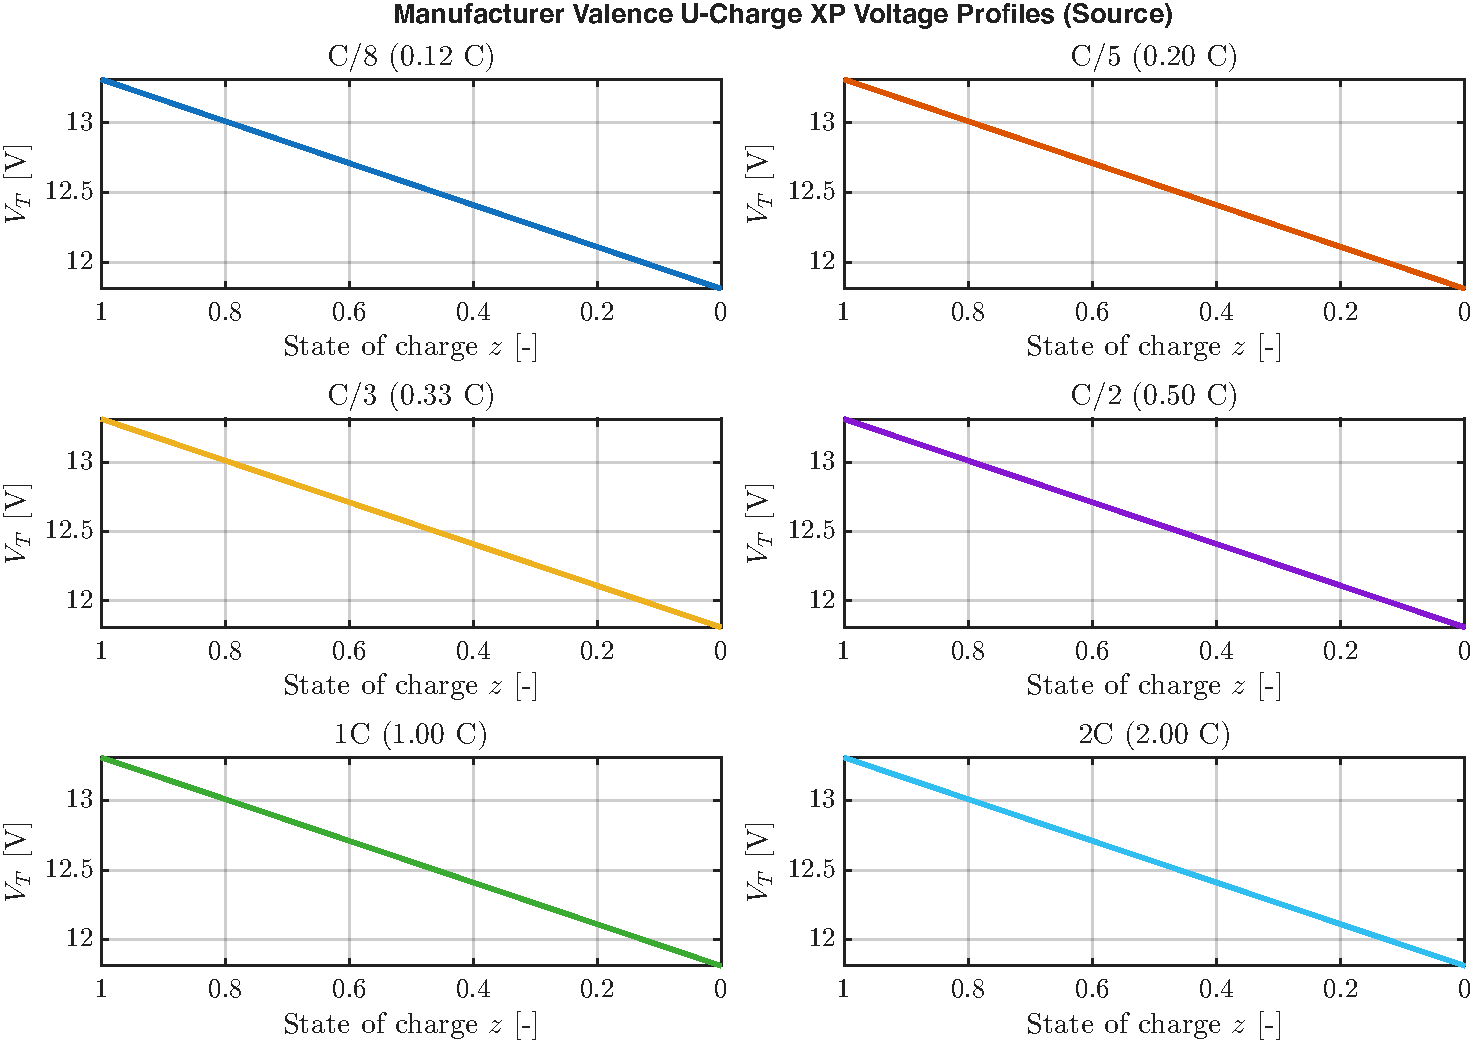
\includegraphics[width=0.82\textwidth]{Figures/valence_voltage_profiles_source.pdf}
\caption{Manufacturer voltage--capacity curves used as the source for the Valence U-Charge XP ECM identification.
The curves report terminal voltage as a function of capacity used at several C-rates.
They support quasi-static voltage identification, but they do not contain pulse/rest information for unique dynamic RC identification.}
\label{fig:exec_source_voltage_profiles}
\end{figure}

After digitisation, the capacity-used coordinate is converted to state of charge using
\begin{equation}
z=1-\frac{q_{\mathrm{used}}}{100}.
\label{eq:exec_capacity_to_soc}
\end{equation}

The digitised curves are then interpolated onto a common SoC grid.

Only the overlapping SoC interval should be used for the regression.

This avoids unsupported extrapolation near the endpoints of individual digitised curves.

\begin{figure}[H]
\centering
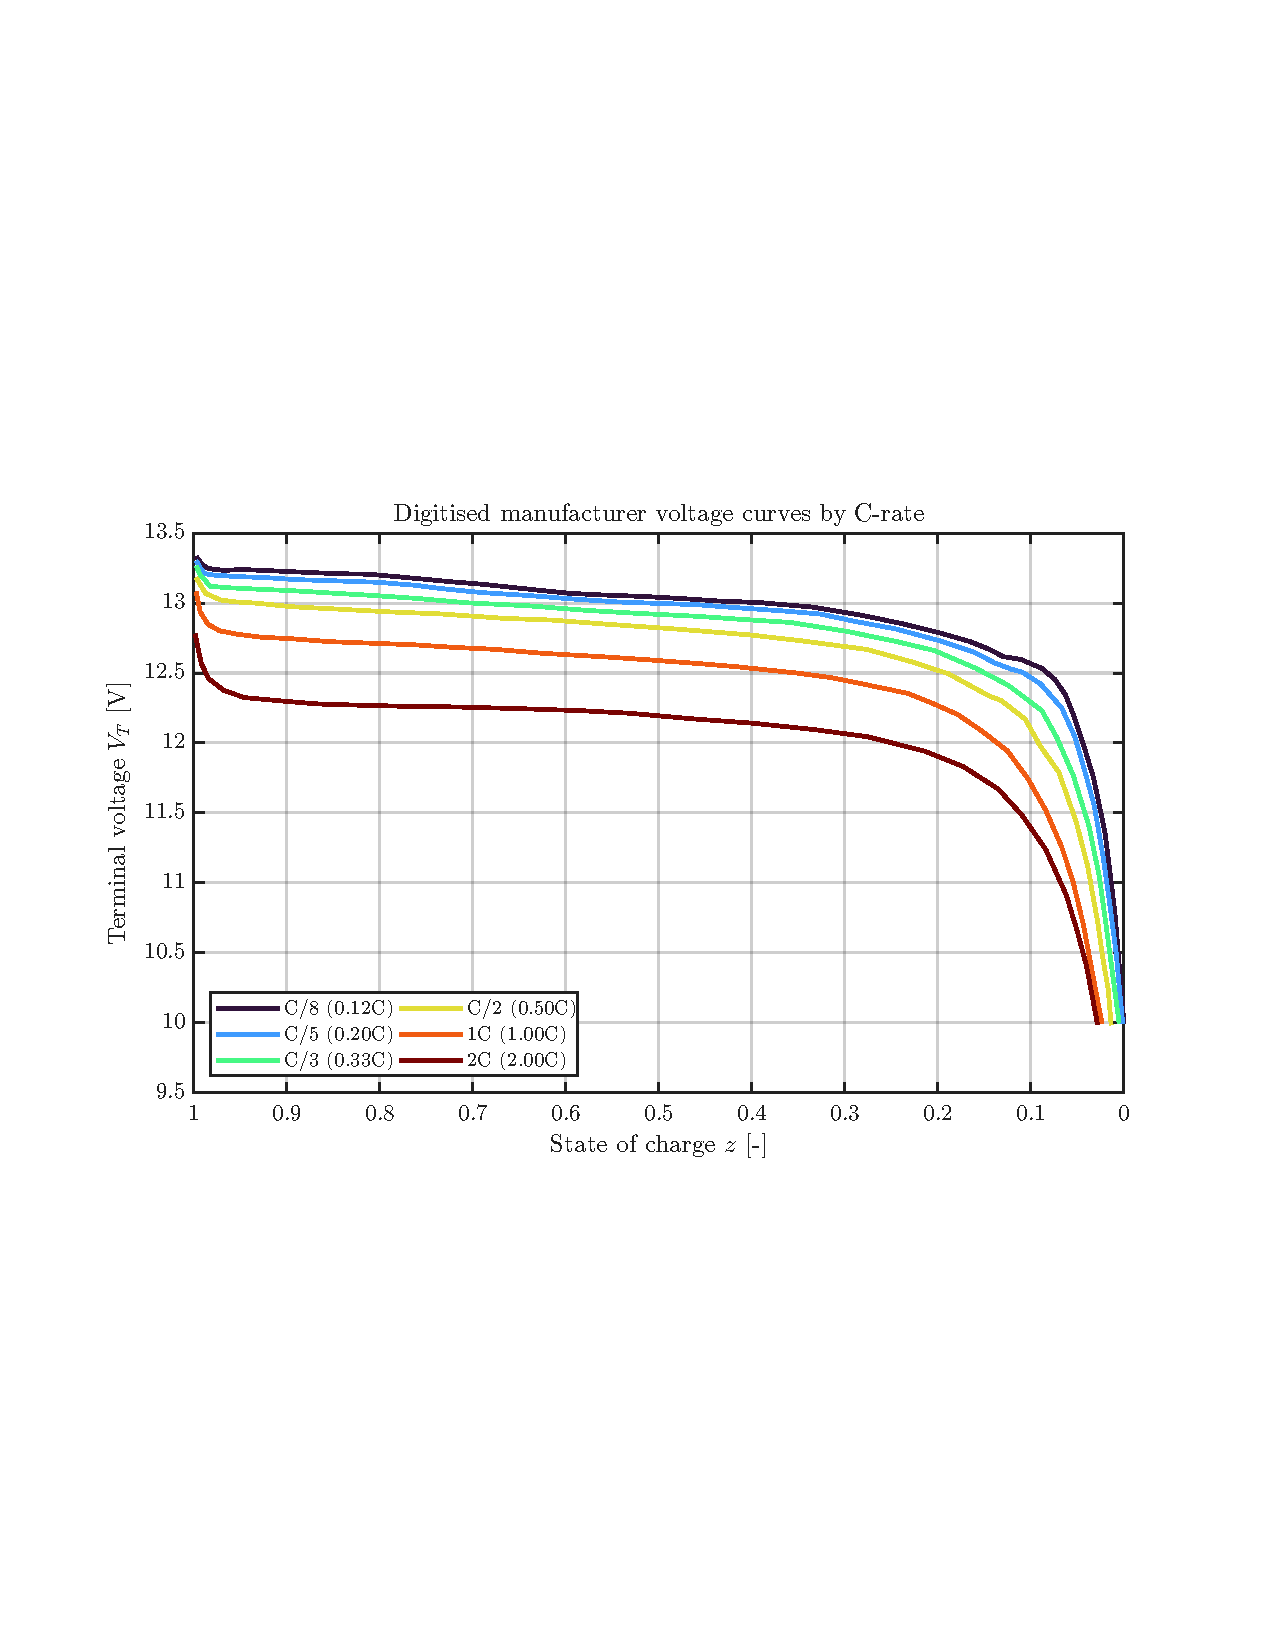
\includegraphics[
    width=0.82\textwidth,
    trim={0.8cm 8.2cm 0.8cm 8.2cm},
    clip
]{Figures/matlab_fig01_digitised_voltage_curves.pdf}
\caption{Digitised voltage curves after conversion to state of charge.
The comparison with Figure~\ref{fig:exec_source_voltage_profiles} provides a visual check that the digitised data preserve the manufacturer-curve structure.}
\label{fig:exec_digitised_voltage_curves}
\end{figure}

% ----------------------------------------------------------
\subsection{Identified Quasi-Static Parameters}

The quasi-static ECM identified by the MATLAB script is
\begin{equation}
\hat{V}_T(z,I)
=
V_{\mathrm{OC}}(z)
-
IR_{\mathrm{eff}}(z).
\label{eq:exec_static_model_repeated}
\end{equation}

At each fixed SoC value, the local voltage--current relation is fitted as
\begin{equation}
V_T(z_i,I_j)
=
\alpha_i+\beta_iI_j+\varepsilon_{ij}.
\label{eq:exec_local_fit}
\end{equation}

The lookup-table entries are then
\begin{equation}
V_{\mathrm{OC}}(z_i)=\alpha_i,
\qquad
R_{\mathrm{eff}}(z_i)=-\beta_i.
\label{eq:exec_lookup_entries}
\end{equation}

The table \(V_{\mathrm{OC}}(z)\) should be interpreted as a zero-current extrapolation from loaded datasheet curves.

It should not be presented as a true rest-measured equilibrium OCV curve.

The table \(R_{\mathrm{eff}}(z)\) should be interpreted as an apparent sustained-discharge resistance.

It should not be presented as the instantaneous ohmic resistance \(R_0(z)\).

\begin{figure}[H]
\centering
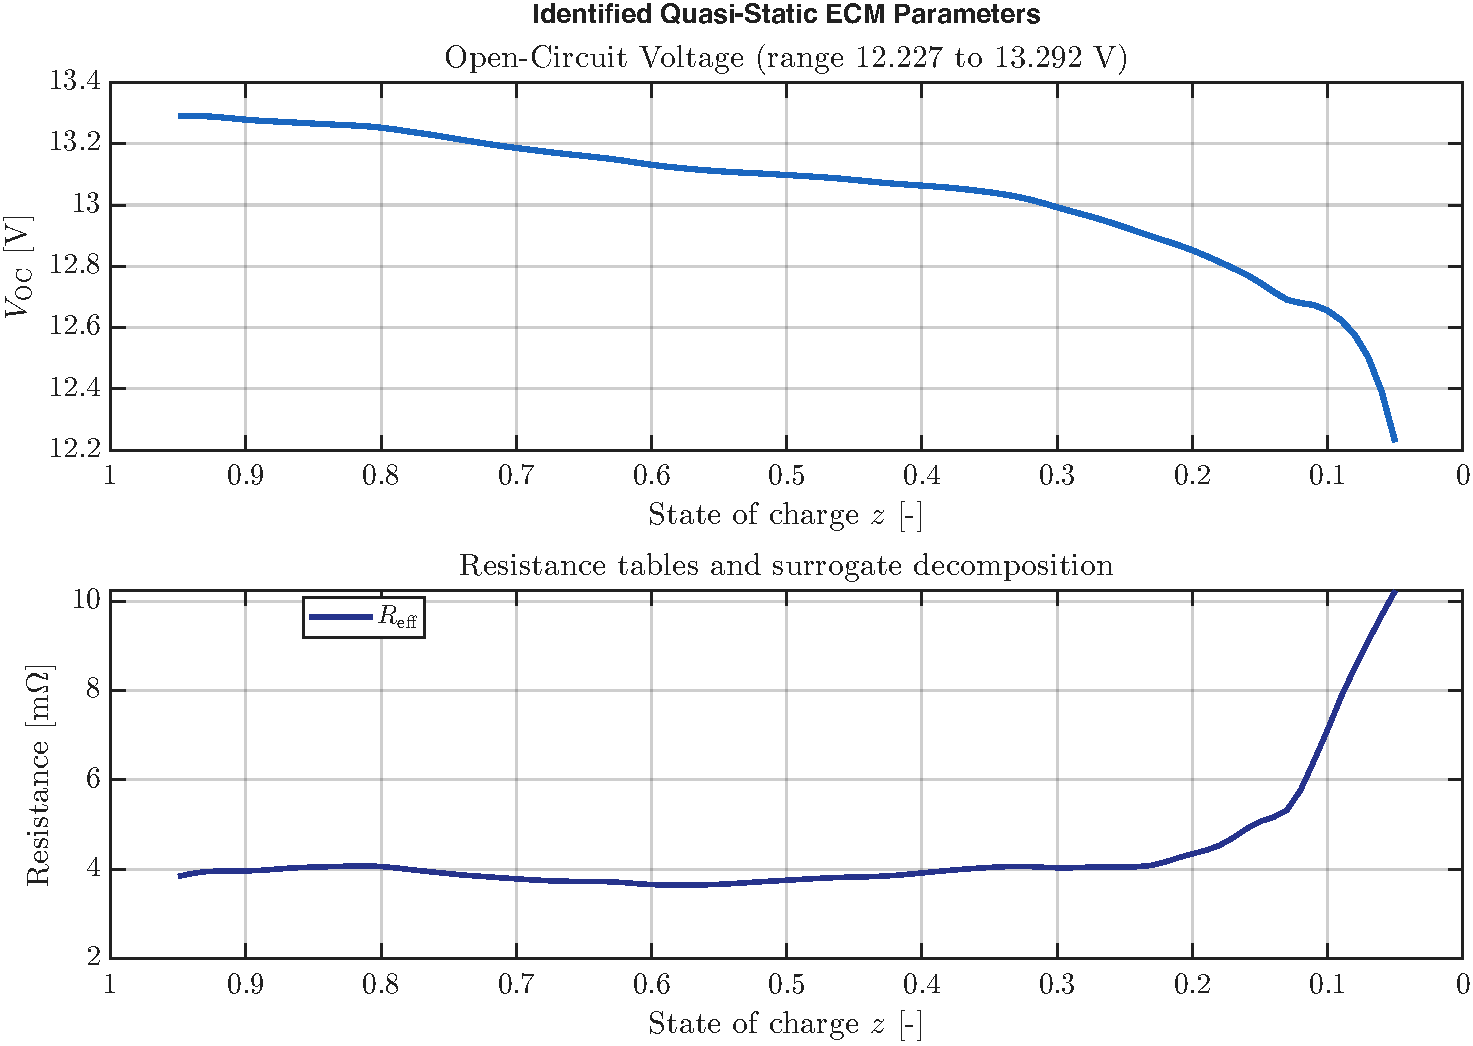
\includegraphics[width=0.86\textwidth]{Figures/matlab_fig02_identified_ocv_reff.pdf}
\caption{Identified quasi-static ECM tables.
Top: datasheet-extrapolated \(V_{\mathrm{OC}}(z)\).
Bottom: apparent effective resistance \(R_{\mathrm{eff}}(z)\).
The fitted resistance includes the combined effect of ohmic and polarisation losses present in the sustained discharge curves.}
\label{fig:exec_identified_ocv_reff}
\end{figure}

The parameter-status classification used in the MATLAB export is reported in Table~\ref{tab:exec_parameter_status_validation}.

This table is essential because it prevents the surrogate 2RC branches from being mistaken for fully identified dynamic parameters.

\begin{table}[H]
\centering
\caption{Parameter status in the exported ECM model.}
\label{tab:exec_parameter_status_validation}
\begin{tabularx}{0.96\textwidth}{@{}L{0.24\textwidth}L{0.30\textwidth}Y@{}}
\toprule
\textbf{Parameter} &
\textbf{Status} &
\textbf{Interpretation} \\
\midrule
\(V_{\mathrm{OC}}(z)\) &
\texttt{datasheet-extrapolated} &
Zero-current intercept obtained from loaded multi-rate discharge curves. \\
\(R_{\mathrm{eff}}(z)\) &
\texttt{identified-apparent} &
Current sensitivity of terminal voltage at fixed SoC. \\
\(R_0(z)\) &
\texttt{datasheet-bounded} &
Initialised using \(R_{\mathrm{DC,max}}\) as a bound or reference value. \\
\(R_1(z)\), \(R_2(z)\) &
\texttt{surrogate} &
Obtained from a documented split of \(R_{\mathrm{eff}}(z)-R_0(z)\). \\
\(C_1(z)\), \(C_2(z)\) &
\texttt{surrogate} &
Computed from assumed time constants and surrogate branch resistances. \\
\(\tau_1\), \(\tau_2\) &
\texttt{assumed} &
Chosen to provide plausible fast and slow relaxation behaviour. \\
\bottomrule
\end{tabularx}
\end{table}

% ----------------------------------------------------------
\subsection{Surrogate 2RC Parameter Initialisation}

The 2RC model used for Simulink implementation is
\begin{equation}
V_T
=
V_{\mathrm{OC}}(z)
-
R_0(z)I
-
V_1
-
V_2.
\label{eq:exec_2rc_voltage}
\end{equation}

The dynamic branch states are
\begin{equation}
\dot{V}_1
=
-\frac{1}{R_1(z)C_1(z)}V_1
+
\frac{1}{C_1(z)}I,
\qquad
\dot{V}_2
=
-\frac{1}{R_2(z)C_2(z)}V_2
+
\frac{1}{C_2(z)}I.
\label{eq:exec_2rc_state_equations}
\end{equation}

Because no pulse/rest data are available, these dynamic parameters are not identified directly.

They are initialised as a physically constrained surrogate.

The recommended ohmic-resistance definition is
\begin{equation}
R_0(z_i)
=
\min
\left[
R_{\mathrm{DC,max}},
\;
\eta_R R_{\mathrm{eff}}(z_i)
\right],
\qquad
0<\eta_R<1.
\label{eq:exec_r0_bounded}
\end{equation}

The remaining apparent polarisation resistance is
\begin{equation}
R_{\mathrm{pol}}(z_i)
=
R_{\mathrm{eff}}(z_i)-R_0(z_i).
\label{eq:exec_rpol}
\end{equation}

The two branch resistances are assigned as
\begin{equation}
R_1(z_i)=\alpha_RR_{\mathrm{pol}}(z_i),
\qquad
R_2(z_i)=(1-\alpha_R)R_{\mathrm{pol}}(z_i),
\qquad
0<\alpha_R<1.
\label{eq:exec_branch_split}
\end{equation}

The capacitances are computed from assumed time constants:
\begin{equation}
C_1(z_i)=\frac{\tau_1}{R_1(z_i)},
\qquad
C_2(z_i)=\frac{\tau_2}{R_2(z_i)},
\qquad
0<\tau_1<\tau_2.
\label{eq:exec_surrogate_capacitances}
\end{equation}

This construction preserves the identified quasi-static voltage drop because
\begin{equation}
R_0(z_i)+R_1(z_i)+R_2(z_i)
=
R_{\mathrm{eff}}(z_i).
\label{eq:exec_surrogate_consistency}
\end{equation}

The transient response, however, remains assumed.

It must therefore be recalibrated if pulse-current and relaxation measurements become available.

\begin{figure}[H]
\centering
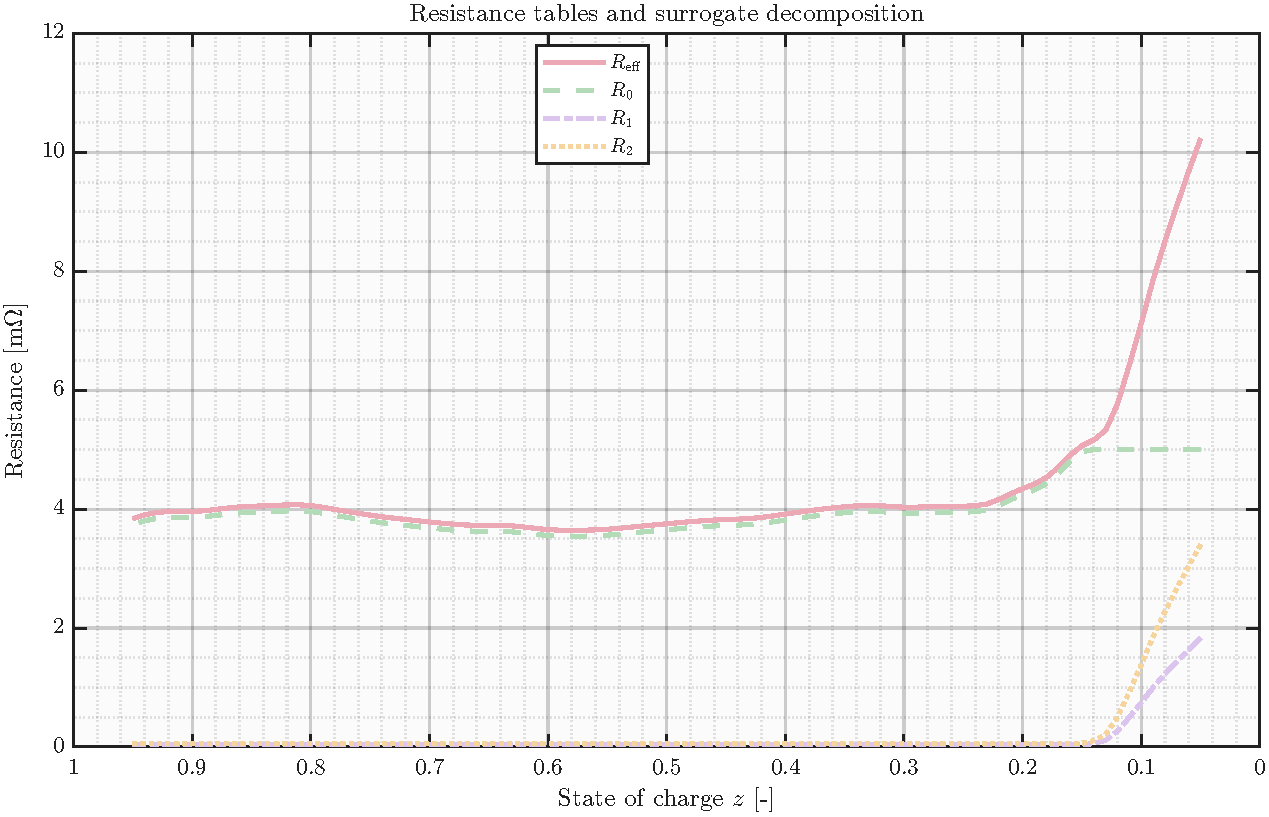
\includegraphics[width=0.86\textwidth]{Figures/matlab_fig03_resistances.pdf}
\caption{Surrogate 2RC lookup tables generated from the identified \(R_{\mathrm{eff}}(z)\), a bounded \(R_0(z)\), an assumed resistance split, and assumed fast and slow time constants.
These tables provide a Simulink-ready dynamic extension, but they are not uniquely identified from the datasheet discharge curves.}
\label{fig:exec_surrogate_2rc_tables}
\end{figure}

% ----------------------------------------------------------
\subsection{Voltage Reconstruction and Residual Diagnostics}

The first validation step reconstructs each voltage curve using
\begin{equation}
\hat{V}_T(z_i,I_j)
=
V_{\mathrm{OC}}(z_i)
-
I_jR_{\mathrm{eff}}(z_i).
\label{eq:exec_reconstructed_voltage}
\end{equation}

The residual is
\begin{equation}
e_{ij}
=
V_T(z_i,I_j)-\hat{V}_T(z_i,I_j).
\label{eq:exec_residual}
\end{equation}

Measured and reconstructed curves should be plotted together before reporting scalar metrics.

This shows whether the model captures the main voltage-shape behaviour and where the largest local errors occur.

\begin{figure}[H]
\centering
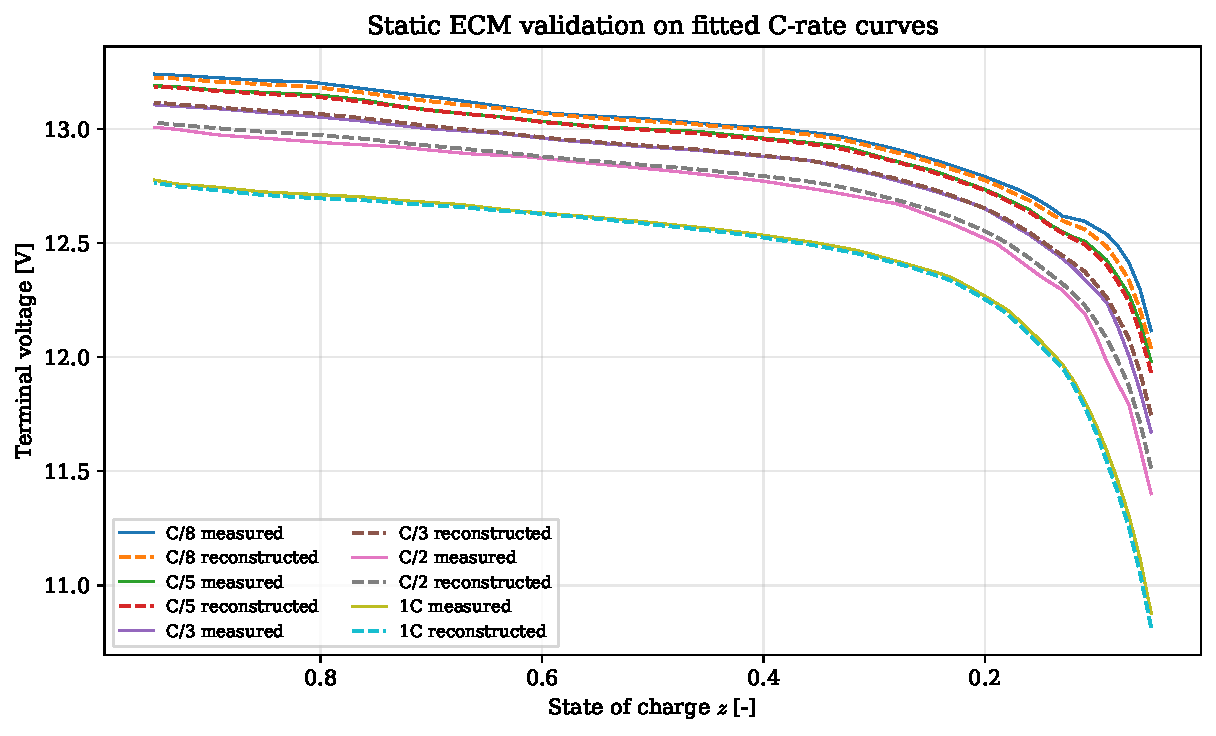
\includegraphics[width=0.88\textwidth]{Figures/matlab_fig03_voltage_reconstruction.pdf}
\caption{Measured and reconstructed voltage curves for the identified quasi-static ECM.
The C/8--1C curves define the main calibration domain.
The 2C curve should be interpreted as a high-current holdout case.}
\label{fig:exec_voltage_reconstruction}
\end{figure}

Residual plots are required because scalar error metrics can hide systematic model-structure errors.

For example, a low RMSE can still coexist with systematic end-of-discharge errors near the voltage knee.

\begin{figure}[H]
\centering
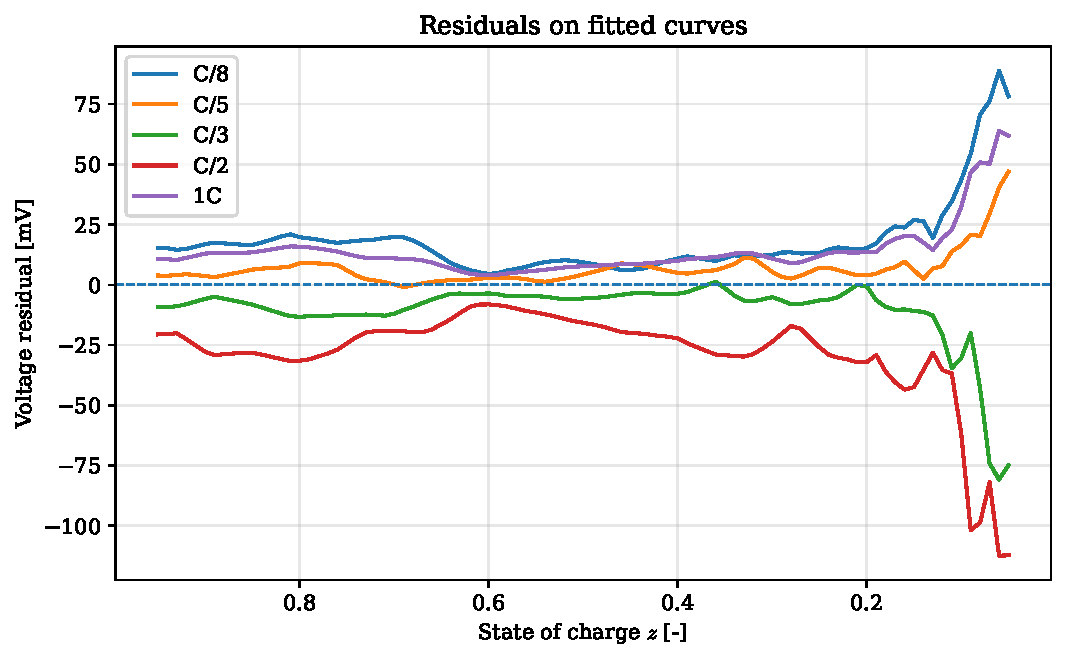
\includegraphics[width=0.88\textwidth]{Figures/matlab_fig04_voltage_residuals.pdf}
\caption{Voltage residuals \(e=V_T-\hat{V}_T\) as a function of SoC.
Residual structure is as important as scalar error metrics.
Systematic residuals near low SoC may indicate voltage-knee behaviour, digitisation uncertainty, high-current extrapolation, or insufficient model flexibility near the end of discharge.}
\label{fig:exec_residuals}
\end{figure}

% ----------------------------------------------------------
\subsection{Validation Metrics}

The scalar validation metrics are defined in Table~\ref{tab:exec_metric_definitions}.

The metrics are intentionally partly redundant.

RMSE penalises large local errors.

MAE reports the typical absolute error.

Bias identifies systematic over- or under-prediction.

The \(95\)th percentile absolute error is useful because it is less sensitive than the maximum error to isolated digitisation artefacts.

The coefficient \(R^2\) measures curve-shape agreement.

\begin{table}[H]
\centering
\caption{Validation metrics used to assess voltage-reconstruction quality.}
\label{tab:exec_metric_definitions}
\begin{tabularx}{0.98\textwidth}{@{}L{0.20\textwidth}L{0.36\textwidth}Y@{}}
\toprule
\textbf{Metric} &
\textbf{Definition} &
\textbf{Interpretation} \\
\midrule
RMSE &
\(\displaystyle \sqrt{\frac{1}{M}\sum_i e_{ij}^2}\) &
Average error with strong penalty on large local mismatch. \\
MAE &
\(\displaystyle \frac{1}{M}\sum_i |e_{ij}|\) &
Typical absolute voltage error. \\
Maximum error &
\(\displaystyle \max_i |e_{ij}|\) &
Worst local mismatch, often near the voltage knee. \\
Bias &
\(\displaystyle \frac{1}{M}\sum_i e_{ij}\) &
Systematic over- or under-prediction. \\
NRMSE &
\(\displaystyle \mathrm{RMSE}/(\max V_{T,j}-\min V_{T,j})\) &
Error normalised by the voltage range of each curve. \\
MAPE &
\(\displaystyle 100M^{-1}\sum_i |e_{ij}/V_T(z_i,I_j)|\) &
Relative voltage error in percent. \\
\(R^2\) &
\(\displaystyle 1-\frac{\sum_i e_{ij}^2}{\sum_i(V_T(z_i,I_j)-\bar{V}_{T,j})^2}\) &
Curve-shape agreement. \\
P95AbsError &
\(\displaystyle \mathrm{percentile}_{95}(|e_{ij}|)\) &
Robust high-error indicator excluding isolated extremes. \\
\bottomrule
\end{tabularx}
\end{table}

For the present dataset, the in-domain fitting curves are reconstructed with small voltage errors.

The 2C curve shows a substantially larger error.

This behaviour is expected because
\begin{equation}
I_{2C}=276\,\mathrm{A}>I_{\max}^{\mathrm{cont}}=150\,\mathrm{A}.
\label{eq:exec_2c_above_continuous}
\end{equation}

The model should therefore be reported as validated primarily for the C/8--1C continuous-current range.

The 2C result should be reported as a stress-test result.

\begin{table}[H]
\centering
\caption{Representative validation metrics for the present dataset.
These values must be regenerated if the digitised curves, smoothing settings, or fitting set are changed.}
\label{tab:exec_current_validation_metrics_snapshot}
\begin{tabular*}{\textwidth}{@{\extracolsep{\fill}} l r l r r r @{}}
\toprule
\textbf{Curve} &
\textbf{Current [A]} &
\textbf{Role} &
\textbf{RMSE [V]} &
\textbf{MAE [V]} &
\textbf{Max error [V]} \\
\midrule
C/8 &  17.25 & Fit & 0.0234 & 0.0179 & 0.0889 \\
C/5 &  27.60 & Fit & 0.0098 & 0.0067 & 0.0470 \\
C/3 &  46.00 & Fit & 0.0174 & 0.0104 & 0.0808 \\
C/2 &  69.00 & Fit & 0.0345 & 0.0281 & 0.1124 \\
1C  & 138.00 & Fit & 0.0177 & 0.0140 & 0.0640 \\
2C  & 276.00 & High-current holdout & 0.3111 & 0.2167 & 1.2288 \\
\bottomrule
\end{tabular*}
\end{table}

The largest in-domain RMSE in Table~\ref{tab:exec_current_validation_metrics_snapshot} is \(0.0345\,\mathrm{V}\), obtained for the C/2 curve.

Therefore, any automated in-domain RMSE gate must be set above this value if the table is meant to support a pass decision.

% ----------------------------------------------------------
\subsection{Automated Acceptance Gates}

The validation suite uses acceptance gates to convert numerical evidence into an explicit model-validity statement.

These gates are not universal battery-modelling standards.

They are project-specific thresholds used to distinguish in-domain fit quality, interpolation robustness, and extrapolation risk.

The recommended gates are reported in Table~\ref{tab:exec_acceptance_gates}.

\begin{table}[H]
\centering
\caption{Acceptance gates used for automated validation.}
\label{tab:exec_acceptance_gates}
\begin{tabularx}{0.96\textwidth}{@{}L{0.36\textwidth}C{0.18\textwidth}Y@{}}
\toprule
\textbf{Gate} &
\textbf{Threshold} &
\textbf{Interpretation} \\
\midrule
Fit RMSE maximum &
\(\leq 0.04\,\mathrm{V}\) &
In-domain average reconstruction quality on C/8--1C. \\
Fit \(R^2\) minimum &
\(\geq 0.98\) &
Curve-shape agreement on fitting curves. \\
LOCO RMSE maximum &
\(\leq 0.08\,\mathrm{V}\) &
Interpolation quality when one C-rate curve is removed. \\
1C extrapolation RMSE maximum &
\(\leq 0.08\,\mathrm{V}\) &
Prediction quality when training only up to C/2. \\
1C extrapolation \(R^2\) minimum &
\(\geq 0.90\) &
Curve-shape preservation under moderate extrapolation. \\
2C holdout RMSE maximum &
\(\leq 0.35\,\mathrm{V}\) &
High-current stress-validation error bound. \\
2C holdout \(R^2\) minimum &
\(\geq 0.00\) &
Minimum non-divergent high-current extrapolation behaviour. \\
Noise robustness at \(5\,\mathrm{mV}\) &
\(\leq 0.09\,\mathrm{V}\) &
Stability against digitisation-level voltage perturbations. \\
Positive \(R_{\mathrm{eff}}\) &
All grid points &
Physical admissibility of the apparent resistance table. \\
Positive surrogate \(R\)-\(C\) parameters &
All grid points &
Physical admissibility of the 2RC surrogate implementation. \\
\bottomrule
\end{tabularx}
\end{table}

The formal automated decision is
\begin{equation}
\texttt{overall PASS}
\iff
\texttt{all mandatory in-domain and physical-admissibility gates pass}.
\label{eq:exec_overall_pass_definition}
\end{equation}

The engineering interpretation must be more nuanced than a single pass/fail label.

A failed 2C holdout gate would not invalidate the C/8--1C quasi-static ECM.

It would restrict the validated domain of use.

% ----------------------------------------------------------
\subsection{Validation Figures}

The validation figures should be reported as individual figures rather than as a dense multi-panel atlas.

Each figure should answer one validation question.

% ----------------------------------------------------------
\subsubsection{Parity Validation}

The parity plot compares measured and reconstructed terminal voltages across the validation dataset.

Points close to the diagonal indicate good voltage reconstruction.

Systematic deviation from the diagonal indicates bias or model-structure error.

\begin{figure}[H]
\centering
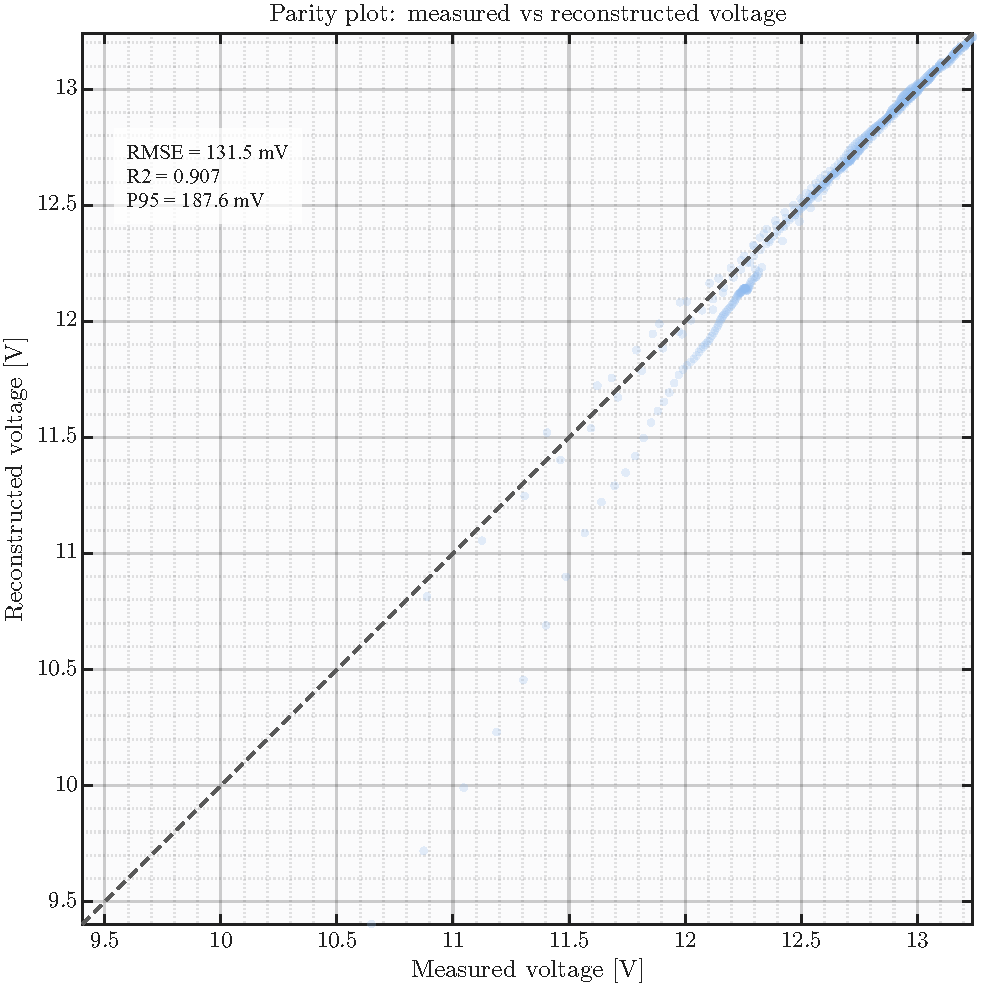
\includegraphics[width=0.82\textwidth]{Figures/matlab_fig08_validation_parity.pdf}
\caption{Parity validation for the identified quasi-static ECM.
Each point compares a measured manufacturer voltage value with the corresponding reconstructed value from
\(\hat{V}_T(z,I)=V_{\mathrm{OC}}(z)-IR_{\mathrm{eff}}(z)\).
Points close to the diagonal indicate good voltage reconstruction.
Systematic deviation from the diagonal would indicate bias or model-structure error.}
\label{fig:exec_validation_parity}
\end{figure}

% ----------------------------------------------------------
\subsubsection{Residual Distribution}

The residual distribution indicates whether the voltage errors are centred around zero and whether a small number of points dominate the RMSE.

A narrow, centred distribution supports the use of the quasi-static ECM over the stated calibration range.

A skewed or heavy-tailed distribution should be discussed.

\begin{figure}[H]
\centering
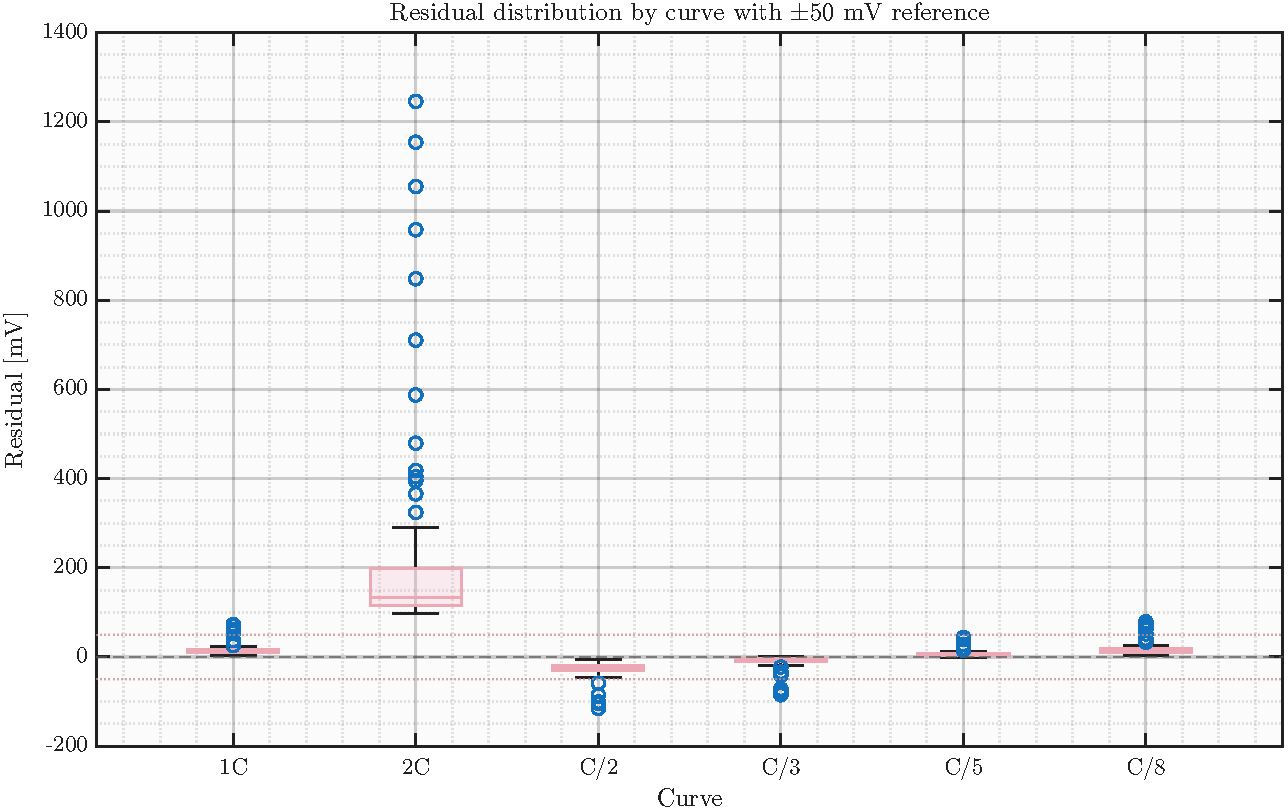
\includegraphics[width=0.82\textwidth]{Figures/matlab_fig09_validation_residual_boxplot.pdf}
\caption{Distribution of voltage residuals.
The plot checks whether reconstruction errors are approximately centred and whether isolated large residuals dominate the validation metrics.}
\label{fig:exec_validation_residual_distribution}
\end{figure}

% ----------------------------------------------------------
\subsubsection{Residual Heatmap}

The residual heatmap localises errors over SoC and C-rate.

This is useful because voltage-reconstruction error is often concentrated near the low-SoC voltage knee or at high current.

\begin{figure}[H]
\centering
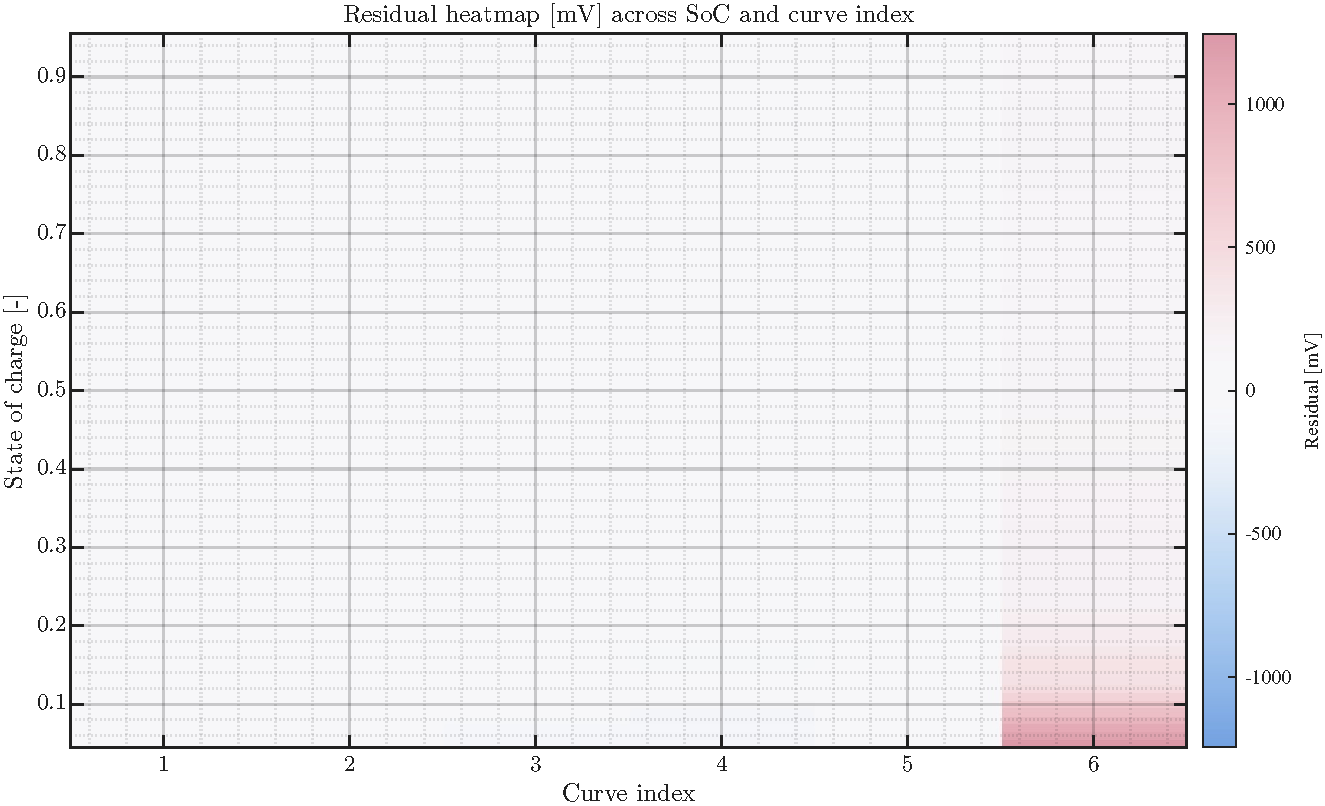
\includegraphics[
    width=0.82\textwidth,
    trim={0.8cm 6.6cm 0.8cm 6.5cm},
    clip
]{Figures/matlab_fig10_validation_residual_heatmap.pdf}
\caption{Residual heatmap over state of charge and C-rate.
The plot indicates where the quasi-static ECM is locally accurate and where the residuals increase.}
\label{fig:exec_validation_residual_heatmap}
\end{figure}

% ----------------------------------------------------------
\subsubsection{Leave-One-Curve-Out Validation}

The leave-one-curve-out test evaluates interpolation robustness between available C-rate curves.

In each test, one C-rate curve is removed from the fitting set.

The model is refitted using the remaining curves.

The removed curve is then reconstructed and its RMSE is recorded.

Low LOCO error indicates that the fitted \(V_{\mathrm{OC}}(z)\) and \(R_{\mathrm{eff}}(z)\) tables are not merely memorising the training curves.

\begin{figure}[H]
\centering
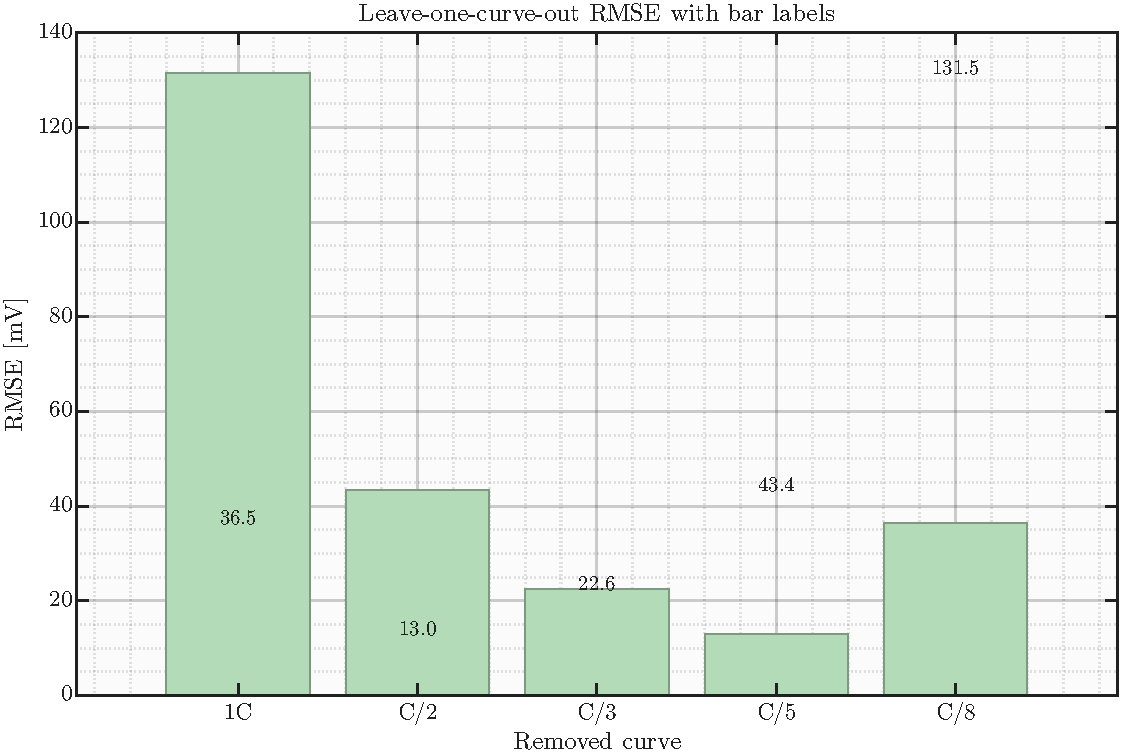
\includegraphics[
    width=0.82\textwidth,
    trim={0.8cm 6.6cm 0.8cm 6.5cm},
    clip
]{Figures/matlab_fig11_validation_loco_rmse.pdf}
\caption{Leave-one-curve-out validation error.
Each bar reports the RMSE obtained when one C-rate curve is removed from the fitting set and reconstructed using the model fitted to the remaining curves.}
\label{fig:exec_validation_loco_rmse}
\end{figure}

% ----------------------------------------------------------
\subsubsection{Noise Robustness}

The noise-robustness test evaluates the sensitivity of the identified parameters and validation errors to digitisation-like perturbations.

This is important because the voltage curves are digitised from a manufacturer figure rather than taken from raw laboratory measurement files.

During the Monte Carlo test, synthetic voltage perturbations are added to the digitised curves.

The identification is then repeated.

A robust workflow should show limited RMSE drift for small voltage perturbations.

\begin{figure}[H]
\centering
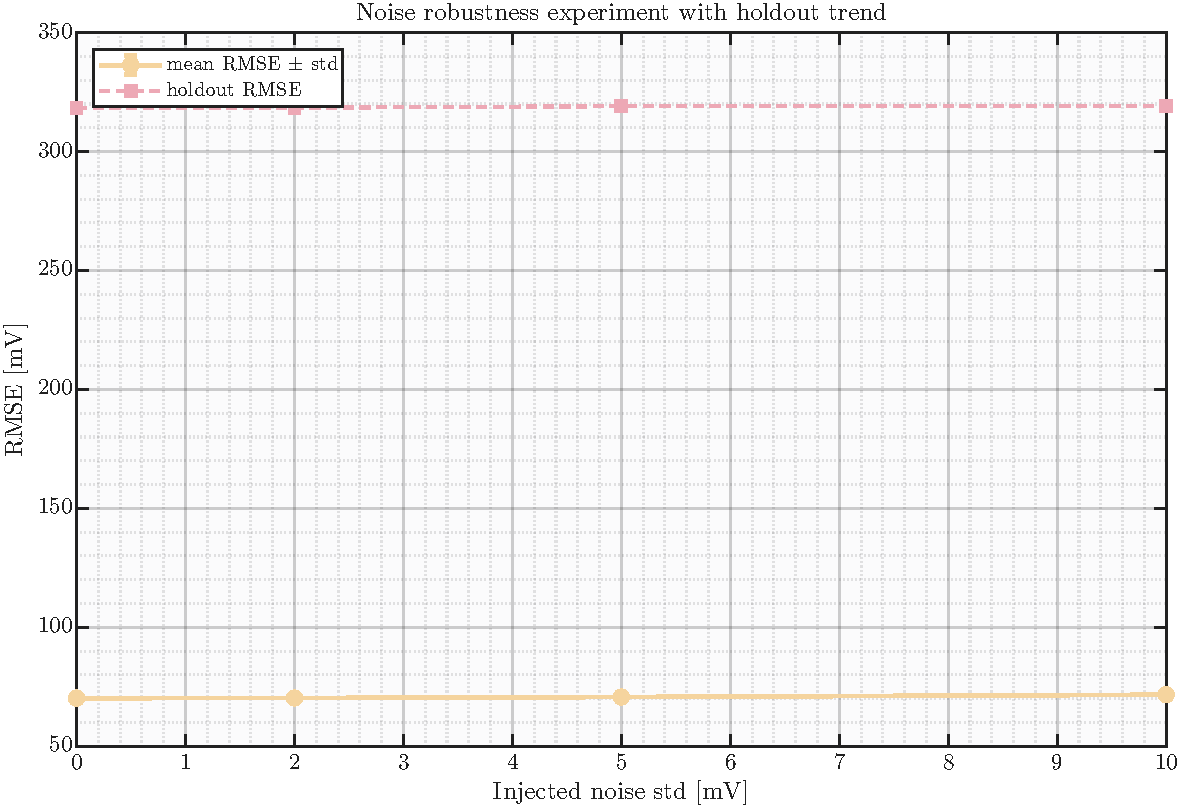
\includegraphics[
    width=0.82\textwidth,
    trim={0.8cm 6.6cm 0.8cm 6.5cm},
    clip
]{Figures/matlab_fig12_validation_noise_robustness.pdf}
\caption{Monte Carlo noise-robustness test.
The plot shows how the validation error changes when small digitisation-like voltage perturbations are added to the input curves.}
\label{fig:exec_validation_noise_robustness}
\end{figure}

% ----------------------------------------------------------
\subsubsection{Extrapolation Stress Tests}

The extrapolation tests evaluate whether the identified model remains predictive when high-current curves are excluded from the fitting set.

These tests are deliberately more demanding than standard in-domain validation.

The first stress test holds out the 1C curve and trains only up to C/2.

The second stress test holds out the 2C curve and trains only up to 1C.

Failure of an extrapolation gate does not invalidate the calibrated C/8--1C model.

It restricts the domain over which the model can safely be claimed as predictive.

\begin{figure}[H]
\centering
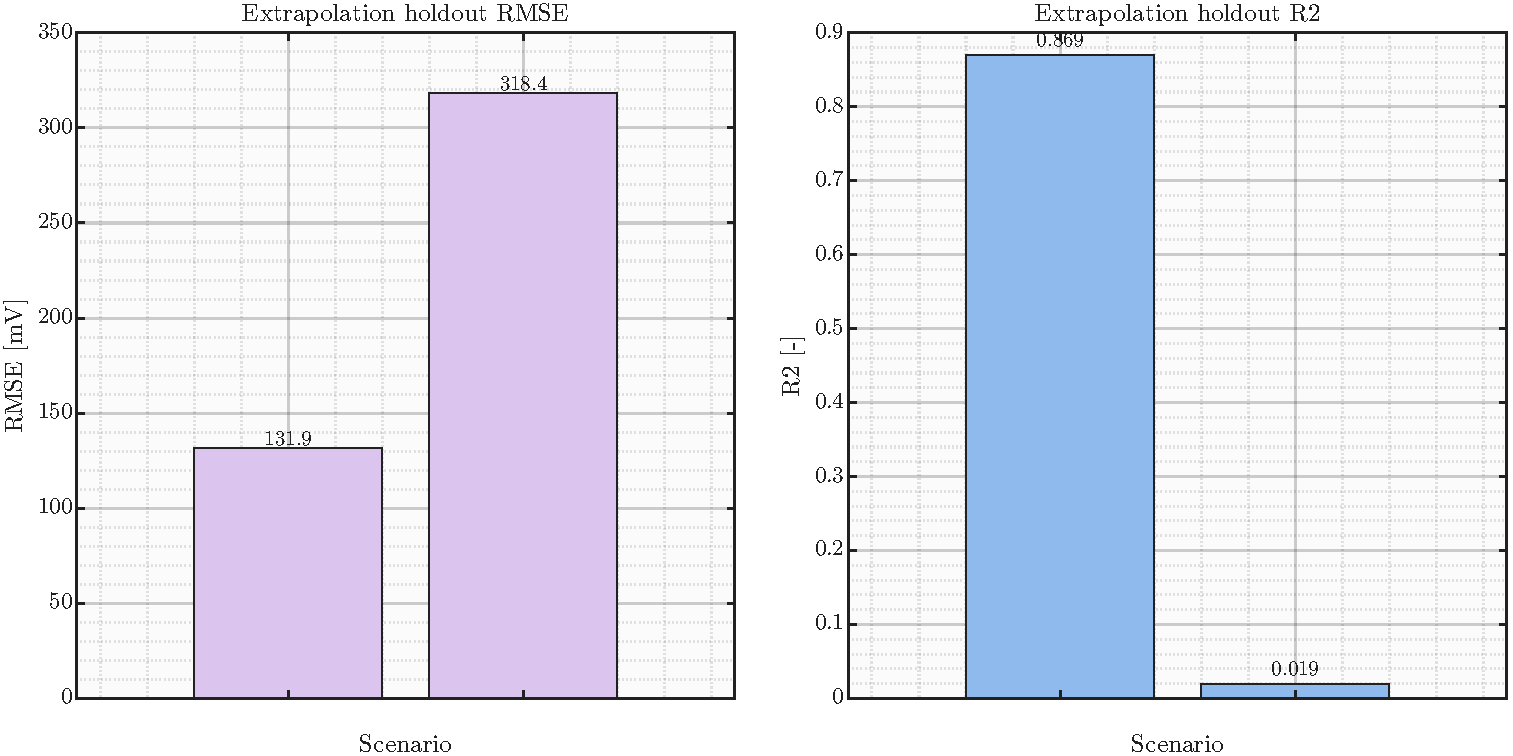
\includegraphics[width=0.82\textwidth]{Figures/matlab_fig13_validation_extrapolation_holdout.pdf}
\caption{Moderate extrapolation stress test.
The model is trained only up to C/2 and used to reconstruct the 1C curve.}
\label{fig:exec_validation_extrapolation_1c}
\end{figure}

\begin{figure}[H]
\centering
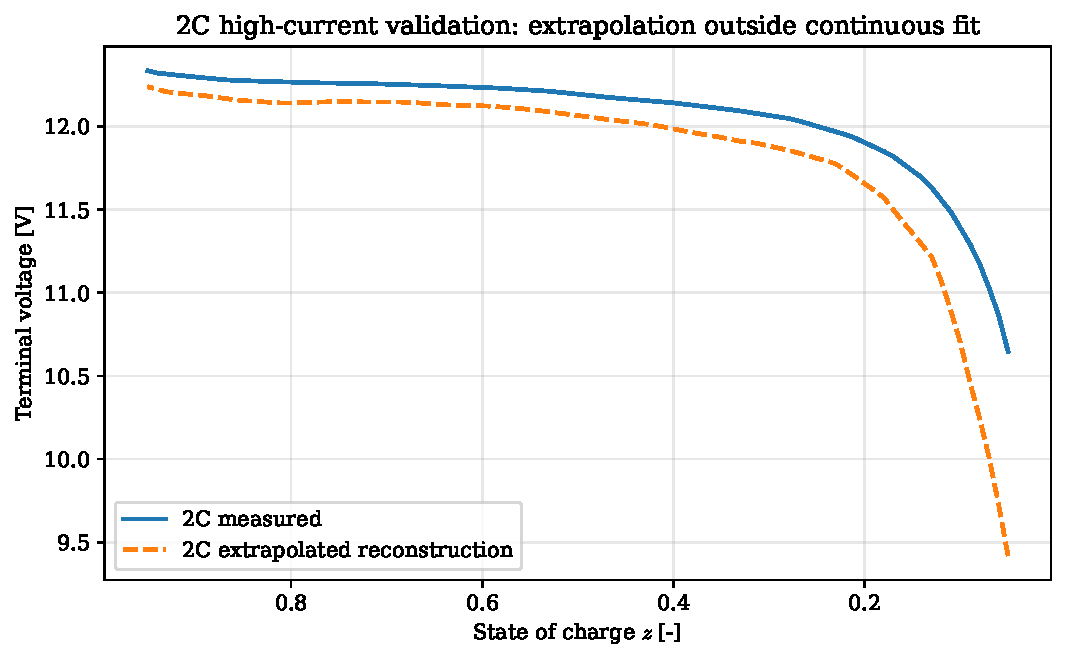
\includegraphics[width=0.82\textwidth]{Figures/fig05_2c_high_current_validation.pdf}
\caption{High-current extrapolation stress test.
The model is trained only up to 1C and used to reconstruct the 2C curve.
This is outside the continuous-current calibration range and should be interpreted as stress validation.}
\label{fig:exec_validation_extrapolation_2c}
\end{figure}

% ----------------------------------------------------------
\subsection{Simulink Implementation Interface}

The exported MATLAB structure should be directly usable by a Simulink battery subsystem.

The quasi-static implementation computes
\begin{equation}
\hat{V}_T
=
V_{\mathrm{OC}}(z)
-
IR_{\mathrm{eff}}(z),
\label{eq:exec_simulink_static_voltage}
\end{equation}
where \(V_{\mathrm{OC}}(z)\) and \(R_{\mathrm{eff}}(z)\) are one-dimensional lookup tables.

The 2RC implementation computes
\begin{equation}
V_T
=
V_{\mathrm{OC}}(z)
-
R_0(z)I
-
V_1
-
V_2,
\label{eq:exec_simulink_2rc_voltage}
\end{equation}
with dynamic states
\begin{equation}
\dot{V}_1
=
-\frac{1}{R_1(z)C_1(z)}V_1
+
\frac{1}{C_1(z)}I,
\qquad
\dot{V}_2
=
-\frac{1}{R_2(z)C_2(z)}V_2
+
\frac{1}{C_2(z)}I.
\label{eq:exec_simulink_2rc_states}
\end{equation}

The SoC update block computes
\begin{equation}
\dot{z}
=
-\frac{I}{3600Q}.
\label{eq:exec_simulink_soc}
\end{equation}

All lookup tables should be protected against extrapolation outside the validated SoC range.

A saturation block should enforce
\begin{equation}
z\in[z_{\min}^{\mathrm{fit}},z_{\max}^{\mathrm{fit}}].
\label{eq:exec_simulink_soc_saturation}
\end{equation}

The current input should also be checked against the validated current range.

For the present parameterisation, the validated continuous-current range is
\begin{equation}
I\in[17.25,138]\,\mathrm{A}
\label{eq:exec_validated_current_range}
\end{equation}
for direct in-domain use.

The 2C condition is outside this range and should be treated as extrapolation.

% ----------------------------------------------------------
\subsection{Pack Scaling for Series and Parallel Modules}

The identified parameters are module-level quantities.

If the model is used for a pack with \(N_s\) modules in series and \(N_p\) parallel strings, the parameters must be scaled before vessel-level simulation.

The pack capacity is
\begin{equation}
Q_{\mathrm{pack}}
=
N_p Q_{\mathrm{module}}.
\label{eq:exec_pack_capacity}
\end{equation}

The pack open-circuit voltage is
\begin{equation}
V_{\mathrm{OC,pack}}(z)
=
N_s V_{\mathrm{OC,module}}(z).
\label{eq:exec_pack_ocv}
\end{equation}

The resistance tables scale as
\begin{equation}
R_{i,\mathrm{pack}}(z)
=
\frac{N_s}{N_p}
R_{i,\mathrm{module}}(z),
\qquad
i\in\{0,1,2\}.
\label{eq:exec_pack_resistances}
\end{equation}

The capacitance tables scale as
\begin{equation}
C_{i,\mathrm{pack}}(z)
=
\frac{N_p}{N_s}
C_{i,\mathrm{module}}(z),
\qquad
i\in\{1,2\}.
\label{eq:exec_pack_capacitances}
\end{equation}

The RC time constants remain unchanged:
\begin{equation}
\tau_i
=
R_iC_i.
\label{eq:exec_pack_time_constants}
\end{equation}

This scaling rule should be applied before using the module model in a vessel-level battery-pack simulation.

% ----------------------------------------------------------
\subsection{Execution Summary}

The complete execution pipeline is summarised in Algorithm~\ref{alg:exec_valence_optimisation}.

The algorithm emphasises that the MATLAB implementation is an identification and validation workflow, not only a plotting script.

\begin{algorithm}[H]
\caption{Valence U27-12XP datasheet-based ECM execution}
\label{alg:exec_valence_optimisation}
\begin{algorithmic}[1]
\Require Digitised voltage--capacity curves and U27-12XP datasheet ratings
\State Set \(Q=\SI{138}{\ampere\hour}\), \(V_{\min}=\SI{10}{\volt}\), and \(V_{\max}=\SI{14.6}{\volt}\)
\State Convert each C-rate to current using \(I_j=C_jQ\)
\State Select C/8 to 1C as the main fitting set
\State Reserve 2C as a high-current holdout curve
\State Convert capacity used to SoC using \(z=1-q_{\mathrm{used}}/100\)
\State Interpolate all fitting curves onto a common SoC grid
\For{each SoC grid point \(z_i\)}
    \State Fit \(V_T(z_i,I_j)=\alpha_i+\beta_iI_j+\varepsilon_{ij}\)
    \State Set \(V_{\mathrm{OC}}(z_i)=\alpha_i\)
    \State Set \(R_{\mathrm{eff}}(z_i)=-\beta_i\)
\EndFor
\State Smooth lookup tables if required
\State Verify \(R_{\mathrm{eff}}(z_i)>0\) and voltage-envelope consistency
\State Initialise \(R_0(z_i)\) using the bounded datasheet-resistance rule
\State Compute \(R_1(z_i)\), \(R_2(z_i)\), \(C_1(z_i)\), and \(C_2(z_i)\) as surrogate 2RC tables
\State Reconstruct all fitting and holdout voltage curves
\State Compute RMSE, MAE, maximum error, \(R^2\), LOCO error, and noise-robustness metrics
\State Apply acceptance gates and report the validated operating domain
\State Export MATLAB and Simulink lookup tables with metadata and parameter-status labels
\end{algorithmic}
\end{algorithm}

The execution produces two outputs.

The first output is the identified quasi-static ECM:
\begin{equation}
\boxed{
\hat{V}_T(z,I)
=
V_{\mathrm{OC}}(z)
-
IR_{\mathrm{eff}}(z).
}
\label{eq:exec_final_static_output}
\end{equation}

The second output is the documented surrogate 2RC implementation:
\begin{equation}
\boxed{
V_T
=
V_{\mathrm{OC}}(z)
-
R_0(z)I
-
V_1
-
V_2.
}
\label{eq:exec_final_dynamic_output}
\end{equation}

Only the first output is directly identified from the datasheet curves.

The second output is a physically constrained dynamic initialisation for Simulink.

The final model-validity statement is therefore:

\begin{quote}
The Valence U27-12XP ECM is validated as a datasheet-based quasi-static voltage model over the C/8--1C continuous-current range covered by the fitting curves.
The 2C result is a high-current stress validation outside the continuous-current calibration range.
The dynamic 2RC branch parameters are surrogate values and should be recalibrated if pulse-current and rest-relaxation measurements become available.
\end{quote}

\clearpage
\newpage
% ==========================================================
\section{Interpretation, Limitations, and Experimental Extension}
\label{sec:interpretation_limitations_extension}

This section interprets the identified ECM parameters as the outcome of an inverse problem.

The previous sections formulated the datasheet-based identification workflow, executed it in MATLAB, and validated the reconstructed terminal-voltage curves.

The purpose here is to clarify what the identified parameters mean physically, what the validation results prove, what they do not prove, and which additional experiments would be required to upgrade the model from a datasheet-based quasi-static ECM to a dynamically identified Thevenin model.

The central point is simple.

A small voltage-reconstruction error does not imply that all equivalent-circuit parameters have been uniquely identified.

A datasheet-based model can reproduce voltage--capacity curves accurately while still being unable to separate instantaneous ohmic losses from transient polarisation losses.

For this reason, the physical interpretation of the result must follow the structure of the inverse problem.

\begin{center}
\begin{tikzpicture}
    \node [
        inner sep=10pt,
        text width=0.85\textwidth,
        align=left,
        font=\small
    ] (text) {
        \textbf{Interpretation principle:} \\
        The credibility of an ECM parameter depends on the information content of the data used to identify it.
        Sustained multi-rate discharge curves identify a quasi-static voltage relation.
        Transient current-step and rest-relaxation measurements are required to identify dynamic RC parameters.
    };
    \draw [TUorange, line width=3pt] (text.north west) -- (text.south west);
\end{tikzpicture}
\end{center}

In this tutorial, the optimisation problem directly identifies the quasi-static voltage model
\begin{equation}
\hat{V}_T(z,I)
=
V_{\mathrm{OC}}(z)
-
IR_{\mathrm{eff}}(z).
\label{eq:interp_static_model}
\end{equation}

The same data do not uniquely identify the dynamic Thevenin model
\begin{equation}
V_T
=
V_{\mathrm{OC}}(z)
-
R_0(z)I
-
V_1
-
V_2.
\label{eq:interp_dynamic_model}
\end{equation}

The dynamic model can be initialised for simulation, but its RC branch parameters remain surrogate quantities unless transient pulse/rest data are added.

% ----------------------------------------------------------
\subsection{Meaning of the Identified Quasi-Static Parameters}

At each fixed SoC value \(z_i\), the local voltage--current regression is
\begin{equation}
V_T(z_i,I_j)
=
\alpha_i
+
\beta_i I_j
+
\varepsilon_{ij}.
\label{eq:interp_local_regression}
\end{equation}

The identified quantities are
\begin{equation}
V_{\mathrm{OC}}(z_i)
=
\alpha_i,
\qquad
R_{\mathrm{eff}}(z_i)
=
-\beta_i.
\label{eq:interp_ocv_reff}
\end{equation}

The intercept \(\alpha_i\) is not a direct rest-voltage measurement.

It is a zero-current extrapolation from loaded discharge curves.

It should therefore be interpreted as a datasheet-extrapolated OCV approximation:
\begin{equation}
V_{\mathrm{OC}}^{\mathrm{fit}}(z)
\neq
V_{\mathrm{OC}}^{\mathrm{equilibrium}}(z)
\qquad
\text{unless rest measurements are available.}
\label{eq:interp_ocv_not_true_equilibrium}
\end{equation}

The slope \(\beta_i\) represents the local voltage sensitivity to current.

The corresponding resistance \(R_{\mathrm{eff}}(z)\) is an apparent sustained-discharge resistance.

It should not be renamed \(R_0(z)\), because it includes more than the instantaneous ohmic voltage drop.

A useful interpretation is
\begin{equation}
R_{\mathrm{eff}}(z)
\approx
R_0(z)
+
R_{\mathrm{ct}}(z)
+
R_{\mathrm{diff}}(z)
+
R_{\mathrm{thermal/rate}}(z),
\label{eq:interp_reff_components}
\end{equation}
where \(R_{\mathrm{ct}}\) denotes charge-transfer effects, \(R_{\mathrm{diff}}\) denotes diffusion-related polarisation, and \(R_{\mathrm{thermal/rate}}\) collects thermal and rate-dependent contributions embedded in the sustained discharge curves.

For the Valence U27-12XP module, the datasheet maximum DC resistance is
\begin{equation}
R_{\mathrm{DC,max}}
=
\SI{5}{\milli\ohm}.
\label{eq:interp_valence_rdc}
\end{equation}

This value is useful as a reference or upper bound for the ohmic component.

It is not equivalent to \(R_{\mathrm{eff}}(z)\).

If the fitted \(R_{\mathrm{eff}}(z)\) exceeds \(\SI{5}{\milli\ohm}\), this is not automatically an inconsistency.

It indicates that the apparent resistance contains voltage-loss mechanisms beyond the datasheet DC resistance.

% ----------------------------------------------------------
\subsection{What the Validation Results Prove}

The validation results prove that the identified quasi-static relation can reconstruct the digitised voltage--capacity curves over the stated calibration domain.

For the fitting curves, the relevant statement is
\begin{equation}
\hat{V}_T(z,I_j)
=
V_{\mathrm{OC}}(z)
-
I_jR_{\mathrm{eff}}(z)
\qquad
j\in\mathcal{J}_{\mathrm{fit}}.
\label{eq:interp_fit_domain_reconstruction}
\end{equation}

If the RMSE, MAE, residual distribution, parity plot, and residual heatmap are satisfactory, then the model is a valid empirical voltage-reconstruction model over the fitted SoC and current range.

The validation also proves that the extracted lookup tables are numerically usable if they satisfy the physical checks
\begin{equation}
R_{\mathrm{eff}}(z)>0,
\qquad
V_{\min}
\leq
\hat{V}_T(z,I)
\leq
V_{\max}.
\label{eq:interp_static_physical_checks}
\end{equation}

The leave-one-curve-out tests provide additional evidence that the model is not only memorising individual C-rate curves.

They test whether the voltage--current slope at fixed SoC is sufficiently robust to predict a removed current level.

The 2C holdout test has a different interpretation.

It checks high-current extrapolation outside the main continuous-current calibration domain.

A larger 2C error is therefore not surprising and should not be interpreted as a failure of the C/8--1C quasi-static ECM.

% ----------------------------------------------------------
\subsection{What the Validation Results Do Not Prove}

The validation results do not prove that the fitted \(V_{\mathrm{OC}}(z)\) is the true thermodynamic equilibrium OCV curve.

They also do not prove that \(R_{\mathrm{eff}}(z)\) is the instantaneous ohmic resistance.

Most importantly, they do not prove that the dynamic RC parameters are uniquely identified.

The reason is structural.

The sustained discharge data provide terminal voltage under load.

They do not contain the instantaneous voltage jump caused by \(R_0\).

They do not contain the relaxation transients needed to estimate \(R_1C_1\) and \(R_2C_2\).

Therefore, the following implication is invalid:
\begin{equation}
\text{small voltage-reconstruction error}
\;\nRightarrow\;
\text{unique dynamic ECM parameters}.
\label{eq:interp_invalid_implication}
\end{equation}

The valid implication drawn from these metrics is therefore strictly bounded.

\begin{center}
% Define the color OUTSIDE the tikzpicture options
\colorlet{TUorange}{orange!80!black}

\begin{tikzpicture}
    \node [
        inner sep=10pt,
        text width=0.85\textwidth,
        align=left,
        font=\small
    ] (text) {
        \textbf{Valid Diagnostic Implication:} \\
        A definitively small voltage-reconstruction error guarantees an accurate quasi-static reconstruction strictly within the validated operational domain.
    };
    \draw [TUorange, line width=3pt] (text.north west) -- (text.south west);
\end{tikzpicture}
\end{center}

This distinction should be stated explicitly in the report and in the MATLAB parameter metadata.

% ----------------------------------------------------------
\subsection{Validated Domain of Use}

The identified model should be used only over the domain supported by the data and validation tests.

For the present Valence U27-12XP tutorial, the primary current-domain statement is
\begin{equation}
I
\in
[17.25,138]\,\mathrm{A}
\label{eq:interp_valid_current_range}
\end{equation}
for direct in-domain use of the fitted C/8--1C curves.

The corresponding operating condition is sustained discharge near the datasheet reference condition.

The 2C curve corresponds to
\begin{equation}
I_{2C}
=
276\,\mathrm{A},
\label{eq:interp_2c_current}
\end{equation}
which exceeds the continuous-current rating of
\begin{equation}
I_{\max}^{\mathrm{cont}}
=
150\,\mathrm{A}.
\label{eq:interp_cont_current_limit}
\end{equation}

The 2C case should therefore be reported as a high-current stress test, not as part of the normal continuous-current calibration domain.

The SoC validity range should also be explicitly stored in the MATLAB parameter structure:
\begin{equation}
z
\in
[z_{\min}^{\mathrm{fit}},z_{\max}^{\mathrm{fit}}].
\label{eq:interp_valid_soc_range}
\end{equation}

The model should not be extrapolated beyond this range without additional validation.

Table~\ref{tab:interp_validity_domains} summarises the recommended validity statement.

\begin{table}[H]
\centering
\caption{Recommended validity-domain statement for the identified ECM.}
\label{tab:interp_validity_domains}
\begin{tabularx}{0.98\textwidth}{@{}L{0.27\textwidth}Y Y@{}}
\toprule
\textbf{Domain} &
\textbf{Supported use} &
\textbf{Caution} \\
\midrule
C/8--1C discharge &
Main quasi-static voltage reconstruction. &
Valid over the fitted SoC range and near the datasheet reference condition. \\
2C discharge &
High-current stress validation. &
Outside the continuous-current calibration domain. \\
Rest voltage &
Not directly measured. &
The fitted \(V_{\mathrm{OC}}\) is a zero-current extrapolation, not a true equilibrium curve. \\
Transient current response &
Not directly validated. &
Requires pulse-current and rest-relaxation experiments. \\
Temperature variation &
Not fully identified. &
Requires tests at multiple controlled temperatures. \\
Ageing and cycle dependence &
Not identified. &
Requires repeated tests over ageing states or cycle count. \\
\bottomrule
\end{tabularx}
\end{table}

% ----------------------------------------------------------
\subsection{Limitations of the Datasheet-Based ECM}

The limitations of the present ECM are consequences of the available data, not failures of the methodology.

The first limitation is digitisation uncertainty.

The voltage curves are extracted from a manufacturer figure, not from raw measurement files.

Small graphical errors can therefore propagate into \(V_{\mathrm{OC}}(z)\), \(R_{\mathrm{eff}}(z)\), and the validation metrics.

The second limitation is the absence of true rest-voltage data.

Without sufficiently long rest periods at known SoC, the equilibrium OCV curve cannot be measured directly.

The third limitation is dynamic non-identifiability.

Without current steps and relaxation intervals, the dynamic split among \(R_0\), \(R_1\), \(C_1\), \(R_2\), and \(C_2\) is not observable.

The fourth limitation is thermal ambiguity.

The sustained discharge curves may include temperature rise and rate-dependent behaviour, but the temperature trajectory is not provided.

The fifth limitation is ageing ambiguity.

The datasheet curves represent a nominal or representative module state.

They do not identify parameter changes with cycle count, calendar ageing, temperature history, or state of health.

These limitations are summarised in Table~\ref{tab:interp_limitations}.

\begin{table}[H]
\centering
\caption{Main limitations of the datasheet-based ECM and their implications.}
\label{tab:interp_limitations}
\begin{tabularx}{0.98\textwidth}{@{}L{0.29\textwidth}Y Y@{}}
\toprule
\textbf{Limitation} &
\textbf{Implication} &
\textbf{Recommended treatment} \\
\midrule
Digitised source curves &
Voltage points contain graphical uncertainty. &
Use smoothing carefully and report residual diagnostics. \\
No rest-voltage data &
True equilibrium OCV is unavailable. &
Label \(V_{\mathrm{OC}}\) as datasheet-extrapolated. \\
No current-step data &
Instantaneous ohmic drop is unavailable. &
Treat \(R_0\) as datasheet-bounded or pulse-identified only if new data exist. \\
No relaxation data &
RC time constants are unavailable. &
Treat \(R_1,C_1,R_2,C_2\) as surrogate parameters. \\
Limited thermal information &
Temperature effects are embedded but not separated. &
Restrict the model to the reference condition unless thermal tests are added. \\
No ageing information &
SoH dependence is not identified. &
Avoid using the model for degradation studies without ageing data. \\
2C exceeds continuous-current rating &
High-current prediction is extrapolative. &
Report 2C as stress validation, not as normal calibration. \\
\bottomrule
\end{tabularx}
\end{table}

% ----------------------------------------------------------
\subsection{Experimental Upgrade Path}

A fully identified dynamic ECM requires additional experiments.

The minimum upgrade path consists of three data layers.

The first layer is an OCV characterisation test.

The module is charged or discharged to selected SoC points and then allowed to rest until the terminal voltage approaches equilibrium.

This provides a direct estimate of
\begin{equation}
V_{\mathrm{OC}}^{\mathrm{equilibrium}}(z).
\label{eq:interp_true_ocv}
\end{equation}

The second layer is a pulse-current test.

At each selected SoC value, a current pulse is applied and the instantaneous voltage jump is measured.

The ohmic resistance can then be estimated as
\begin{equation}
R_0(z_i)
=
\frac{\Delta V_{\mathrm{inst}}(z_i)}{\Delta I}.
\label{eq:interp_r0_from_pulse}
\end{equation}

The third layer is a rest-relaxation test.

After the pulse, the current is removed and the voltage relaxation is recorded.

For a 2RC model, the relaxation voltage can be approximated as
\begin{equation}
\Delta V_{\mathrm{relax}}(t)
=
A_1\exp\left(-\frac{t}{\tau_1}\right)
+
A_2\exp\left(-\frac{t}{\tau_2}\right),
\label{eq:interp_relaxation_two_exponentials}
\end{equation}
where
\begin{equation}
\tau_1=R_1C_1,
\qquad
\tau_2=R_2C_2.
\label{eq:interp_time_constants_from_relaxation}
\end{equation}

Once \(R_0\), \(\tau_1\), and \(\tau_2\) are observable, the RC branch parameters can be estimated using nonlinear least squares over the full pulse/rest voltage response.

The dynamic identification problem becomes
\begin{equation}
\min_{\vect{\theta}_{\mathrm{dyn}}}
\sum_{k=1}^{N}
\left[
V_{T,k}^{\mathrm{meas}}
-
V_{T,k}^{\mathrm{model}}
\left(
\vect{\theta}_{\mathrm{dyn}}
\right)
\right]^2,
\label{eq:interp_dynamic_upgrade_objective}
\end{equation}
with
\begin{equation}
\vect{\theta}_{\mathrm{dyn}}
=
\begin{bmatrix}
R_0 & R_1 & C_1 & R_2 & C_2
\end{bmatrix}^{\top}.
\label{eq:interp_dynamic_upgrade_theta}
\end{equation}

This upgraded dataset would convert the 2RC model from a surrogate dynamic implementation into a calibrated dynamic model.

Table~\ref{tab:interp_experimental_upgrade} summarises the experimental upgrade path.

\begin{table}[H]
\centering
\caption{Experimental upgrade path from datasheet-based ECM to dynamically identified Thevenin ECM.}
\label{tab:interp_experimental_upgrade}
\begin{tabularx}{0.98\textwidth}{@{}L{0.25\textwidth}Y Y@{}}
\toprule
\textbf{Experiment} &
\textbf{Measured information} &
\textbf{Parameters enabled} \\
\midrule
Rest OCV test &
Equilibrium voltage after long rest at each SoC. &
True \(V_{\mathrm{OC}}^{\mathrm{equilibrium}}(z)\). \\
Current-pulse test &
Instantaneous voltage jump after a current step. &
\(R_0(z)\). \\
Pulse/rest relaxation test &
Voltage relaxation after current removal. &
\(\tau_1(z)\), \(\tau_2(z)\), and dynamic branch separation. \\
Multi-current pulse tests &
Dynamic response at different current amplitudes. &
Current-dependence and nonlinear resistance effects. \\
Temperature-controlled tests &
OCV and pulse response at different temperatures. &
Thermal dependence of \(V_{\mathrm{OC}}\), \(R_0\), \(R_1\), \(C_1\), \(R_2\), and \(C_2\). \\
Ageing-state tests &
Repeated tests at different SoH levels. &
Ageing-dependent ECM tables. \\
\bottomrule
\end{tabularx}
\end{table}

% ----------------------------------------------------------
\subsection{Recommended Upgrade Protocol}

A practical experimental protocol for upgrading the model is as follows.

First, define a set of SoC grid points,
\begin{equation}
z_i
\in
\{1.0,0.9,0.8,\ldots,0.1\}.
\label{eq:interp_upgrade_soc_grid}
\end{equation}

Second, bring the module to each SoC point using a controlled charge or discharge procedure.

Third, rest the module until the terminal-voltage drift is below a selected threshold.

A practical criterion is
\begin{equation}
\left|
\frac{\mathrm{d}V_T}{\mathrm{d}t}
\right|
<
\epsilon_V,
\label{eq:interp_rest_criterion}
\end{equation}
where \(\epsilon_V\) is a small voltage-drift threshold.

Fourth, apply one or more current pulses.

For each pulse, record the pre-pulse voltage, the instantaneous voltage jump, the loaded voltage response, the post-pulse relaxation, current, temperature, and time.

Fifth, fit \(R_0(z_i)\) from the instantaneous jump and fit the RC branches from the transient response.

Sixth, repeat the procedure at multiple temperatures if a thermal ECM is required.

Seventh, repeat the procedure at different ageing states if degradation-aware simulation is required.

This protocol is more demanding than datasheet-based identification, but it is the correct route when the model is intended for transient voltage prediction, observer design, BMS estimation, or degradation analysis.

% ----------------------------------------------------------
\subsection{Model-Use Recommendations}

The model produced in this tutorial is appropriate for preliminary system-level studies.

It is suitable for estimating terminal voltage, current, and SoC evolution in early-stage marine energy-system simulations.

It is also suitable for teaching the relationship between datasheet curves, ECM lookup tables, and Simulink implementation.

However, it should not be used without qualification for applications that require accurate transient voltage dynamics.

Examples include high-bandwidth current control, online state estimation, impedance-sensitive power-electronics studies, thermal runaway analysis, and degradation-aware BMS design.

For these applications, the model must be upgraded using pulse/rest and temperature-controlled data.

The recommended use cases are summarised in Table~\ref{tab:interp_model_use_recommendations}.

\begin{table}[H]
\centering
\caption{Recommended use of the datasheet-based ECM.}
\label{tab:interp_model_use_recommendations}
\begin{tabularx}{0.98\textwidth}{@{}L{0.32\textwidth}Y Y@{}}
\toprule
\textbf{Use case} &
\textbf{Suitability} &
\textbf{Comment} \\
\midrule
Teaching ECM principles &
Suitable. &
The workflow clearly links datasheet curves to model parameters. \\
Preliminary energy-management simulation &
Suitable with stated limits. &
Use within the validated current and SoC domain. \\
Module-to-pack scaling exercises &
Suitable. &
Apply correct series/parallel scaling of voltage, resistance, and capacitance. \\
Steady or slowly varying load studies &
Suitable. &
The quasi-static voltage relation is the directly identified part of the model. \\
Transient voltage prediction &
Limited. &
Requires pulse/rest validation. \\
BMS observer design &
Limited. &
Requires dynamically identified RC branches and measurement-noise modelling. \\
Thermal studies &
Limited. &
Requires temperature-dependent parameter maps. \\
Ageing or degradation studies &
Not sufficient by itself. &
Requires SoH-dependent test data. \\
\bottomrule
\end{tabularx}
\end{table}

% ----------------------------------------------------------
\subsection{Final Interpretation Statement}

The final report should include the following interpretation statement.

\begin{quote}
The Valence U27-12XP ECM was parameterised from manufacturer voltage--capacity curves measured at multiple C-rates.
The open-circuit voltage table was obtained by zero-current extrapolation at fixed SoC and should be interpreted as a datasheet-extrapolated OCV approximation.
The effective resistance table was identified from the terminal-voltage slope with respect to current and should be interpreted as an apparent sustained-discharge resistance.
The fitted \(R_{\mathrm{eff}}(z)\) is not the instantaneous ohmic resistance \(R_0(z)\).
The 2RC dynamic parameters were initialised using a bounded \(R_0(z)\), a documented split of \(R_{\mathrm{eff}}(z)-R_0(z)\), and assumed fast and slow time constants.
They are therefore surrogate dynamic parameters until calibrated against pulse-current and rest-relaxation data.
\end{quote}

% ----------------------------------------------------------
\subsection{Engineering Conclusion}

The datasheet-based ECM is a defensible and useful model if its validity domain is stated clearly.

Its directly identified output is the quasi-static voltage relation
\begin{equation}
\boxed{
\hat{V}_T(z,I)
=
V_{\mathrm{OC}}(z)
-
IR_{\mathrm{eff}}(z).
}
\label{eq:interp_final_static_model}
\end{equation}

Its dynamic 2RC implementation is an extension for simulation convenience:
\begin{equation}
\boxed{
V_T
=
V_{\mathrm{OC}}(z)
-
R_0(z)I
-
V_1
-
V_2.
}
\label{eq:interp_final_dynamic_model}
\end{equation}

The first model is identified from the datasheet curves.

The second model is a physically constrained surrogate unless additional dynamic experiments are performed.

The essential conclusion is therefore
\begin{equation}
\boxed{
\text{the datasheet identifies a quasi-static ECM, not a fully calibrated dynamic Thevenin ECM.}
}
\label{eq:interp_final_conclusion}
\end{equation}

\clearpage
\newpage
% ==========================================================
\section{Final Verification Checklist}
\label{sec:final_verification_checklist}

Before the ECM parameter file is exported and used in MATLAB or Simulink, the complete parameter set must pass a final verification check.

Verification is different from validation.

Validation checks agreement with the digitised voltage data.

Verification checks whether the exported parameter set is physically admissible, numerically safe, and correctly documented.

This distinction is important because a model may reproduce the digitised curves while still containing unsafe lookup-table values, missing metadata, or incorrectly labelled surrogate parameters.

The final verification checklist is given in Table~\ref{tab:final_verification_checklist}.

\begin{table}[H]
\centering
\caption{Final verification checklist before MATLAB and Simulink export.}
\label{tab:final_verification_checklist}
\begin{tabularx}{0.98\textwidth}{@{}L{0.31\textwidth}Y Y@{}}
\toprule
\textbf{Check} &
\textbf{Mathematical or implementation condition} &
\textbf{Purpose} \\
\midrule
Positive effective resistance &
\(R_{\mathrm{eff}}(z_i)>0\) for all \(z_i\). &
Prevents non-physical voltage increase with discharge current. \\
Datasheet-bounded ohmic resistance &
\(0<R_0(z_i)\leq R_{\mathrm{eff}}(z_i)\) for all \(z_i\). &
Ensures that the ohmic component does not exceed the total apparent resistance. \\
Positive RC branch resistances &
\(R_1(z_i)>0\) and \(R_2(z_i)>0\) for all \(z_i\). &
Ensures physically meaningful polarisation branches. \\
Positive RC capacitances &
\(C_1(z_i)>0\) and \(C_2(z_i)>0\) for all \(z_i\). &
Ensures stable dynamic states in the surrogate 2RC model. \\
Time-constant ordering &
\(0<\tau_1<\tau_2\). &
Preserves the interpretation of fast and slow relaxation modes. \\
Surrogate resistance consistency &
\(R_0(z_i)+R_1(z_i)+R_2(z_i)=R_{\mathrm{eff}}(z_i)\). &
Ensures that the 2RC surrogate preserves the identified quasi-static voltage drop. \\
Voltage envelope &
\(V_{\min}\leq \hat{V}_T(z_i,I_j)\leq V_{\max}\) over the validated domain. &
Checks consistency with datasheet operating limits. \\
SoC validity range &
\(z_i\in[z_{\min}^{\mathrm{fit}},z_{\max}^{\mathrm{fit}}]\). &
Prevents unsupported lookup-table extrapolation. \\
Current validity range &
\(I_j\leq I_{\max}^{\mathrm{cont}}\) for the main fitting curves. &
Ensures that the primary calibration remains inside the continuous-current envelope. \\
2C treatment &
The 2C curve is labelled as high-current holdout or stress validation. &
Prevents high-current extrapolation from being misreported as normal calibration. \\
OCV status label &
\(V_{\mathrm{OC}}(z)\) is labelled as \texttt{datasheet-extrapolated}. &
Prevents the fitted zero-current intercept from being mistaken for rest-measured equilibrium OCV. \\
Resistance status label &
\(R_{\mathrm{eff}}(z)\) is labelled as \texttt{identified-apparent}. &
Prevents the fitted current-sensitivity from being mistaken for pure ohmic resistance. \\
Dynamic-parameter status labels &
\(R_0,R_1,C_1,R_2,C_2\) have explicit metadata labels. &
Prevents surrogate dynamic parameters from being mistaken for pulse-identified parameters. \\
Metadata completeness &
Source, module, capacity, limits, validity ranges, and identification notes are present. &
Supports reproducibility and future model revision. \\
Figure availability &
All referenced PDF figures exist and are included directly. &
Prevents hidden placeholder panels in the final report. \\
Reference integration &
All bibliography entries are cited at least once in the text. &
Avoids an uncited reference list and clarifies the role of each source. \\
\bottomrule
\end{tabularx}
\end{table}

The exported model should be considered ready for teaching and preliminary simulation only if the mandatory checks pass.

The mandatory checks are positivity, voltage-envelope consistency, validity-range documentation, parameter-status metadata, and surrogate resistance consistency.

A failed high-current 2C stress check does not invalidate the in-domain C/8--1C quasi-static model.

It only restricts the validated current range.

The final model-validity statement should therefore be written as
\begin{quote}
The exported Valence U27-12XP ECM is validated as a datasheet-based quasi-static voltage model over the C/8--1C continuous-current range and over the SoC interval covered by the digitised fitting curves.
The 2RC dynamic extension is a physically constrained surrogate implementation.
It should not be interpreted as a fully identified dynamic Thevenin model unless pulse-current and rest-relaxation measurements are added.
\end{quote}

\clearpage
\newpage

% ==========================================================
\begin{thebibliography}{99}

% ----------------------------------------------------------
% Manufacturer data
% ----------------------------------------------------------

\bibitem{valence_xp_datasheet}
Valence Technology,
\textit{U-Charge XP Battery Modules Datasheet},
July 2011.
Available in the tutorial data package as \texttt{XP\_Module\_Datasheet.pdf}.

% ----------------------------------------------------------
% Battery equivalent-circuit modelling and BMS references
% ----------------------------------------------------------

\bibitem{chen_rincon_mora_2006}
M.~Chen and G.~A. Rinc\'on-Mora,
``Accurate electrical battery model capable of predicting runtime and I--V performance,''
\textit{IEEE Transactions on Energy Conversion},
vol.~21,
no.~2,
pp.~504--511,
2006.
doi:
\url{https://doi.org/10.1109/TEC.2006.874229}.

\bibitem{he_xiong_fan_2011}
H.~He, R.~Xiong, and J.~Fan,
``Evaluation of lithium-ion battery equivalent circuit models for state of charge estimation by an experimental approach,''
\textit{Energies},
vol.~4,
no.~4,
pp.~582--598,
2011.
doi:
\url{https://doi.org/10.3390/en4040582}.

\bibitem{hu_li_peng_2012}
X.~Hu, S.~Li, and H.~Peng,
``A comparative study of equivalent circuit models for Li-ion batteries,''
\textit{Journal of Power Sources},
vol.~198,
pp.~359--367,
2012.
doi:
\url{https://doi.org/10.1016/j.jpowsour.2011.10.013}.

\bibitem{einhorn_conte_kral_fleig_2011}
M.~Einhorn, F.~V. Conte, C.~Kral, and J.~Fleig,
``Comparison of electrical battery models using a numerically optimized parameterization method,''
in \textit{Proceedings of the 2011 IEEE Vehicle Power and Propulsion Conference},
Chicago, IL, USA,
2011.
doi:
\url{https://doi.org/10.1109/VPPC.2011.6043060}.

\bibitem{plett_bms_vol1}
G.~L. Plett,
\textit{Battery Management Systems, Volume I: Battery Modeling}.
Artech House,
Norwood, MA,
2015.
ISBN:
\texttt{978-1-63081-023-8}.

\bibitem{plett_bms_vol2}
G.~L. Plett,
\textit{Battery Management Systems, Volume II: Equivalent-Circuit Methods}.
Artech House,
Norwood, MA,
2015.
ISBN:
\texttt{978-1-63081-027-6}.

% ----------------------------------------------------------
% System identification and optimisation references
% ----------------------------------------------------------

\bibitem{ljung_system_identification}
L.~Ljung,
\textit{System Identification: Theory for the User},
2nd~ed.
Prentice Hall,
Upper Saddle River, NJ,
1999.
ISBN:
\texttt{0-13-656695-2}.

\bibitem{boyd_vandenberghe_convex}
S.~Boyd and L.~Vandenberghe,
\textit{Convex Optimization}.
Cambridge University Press,
Cambridge,
2004.
Available online:
\url{https://web.stanford.edu/~boyd/cvxbook/}.

\bibitem{nocedal_wright_numerical}
J.~Nocedal and S.~J. Wright,
\textit{Numerical Optimization},
2nd~ed.
Springer,
New York,
2006.
doi:
\url{https://doi.org/10.1007/978-0-387-40065-5}.

\end{thebibliography}

\end{document}
